%% TITLE	Bioengineering Science 2 (Heat and Mass Transport) - Notes
%% DATE		- 20/09/2023
%% AUTHOR	BINGHUAN W LI (Dept. Chemical Eng/Bio Eng, Imperial)

%% compiled in XeLaTeX with Tex Live version 2023.

\documentclass[12pt, a4paper]{article}
\usepackage[top=2.5cm, bottom=1.5cm, left=2.5cm, right=2.5cm]{geometry}
\usepackage[utf8]{inputenc}
\usepackage[english]{babel}

\usepackage{cancel}

\usepackage{tcolorbox}
\tcbuselibrary{breakable}

\usepackage{graphicx}
 
\usepackage{tikzducks}
\usepackage{circuitikz}

\usepackage{hyperref}

\usepackage{wrapfig}
\usepackage{graphicx}
\usepackage{fancyhdr}
\usepackage{xcolor}

\usepackage{fontspec}
    \setmainfont{Times New Roman}
\usepackage{newtxmath}
\usepackage{bm}

\usepackage[font={small,it}]{caption}

\usepackage{float}

\usepackage{appendix}

\definecolor{linkcolour}{rgb}{0,0.2,0.6}
\usepackage{hyperref}
\hypersetup{colorlinks,breaklinks,urlcolor=linkcolour, linkcolor=linkcolour,citecolor=black }

\DeclareMathSizes{12}{12}{7}{7}
\usepackage{booktabs,nicematrix}

\usepackage{adjustbox}

\usepackage{booktabs}
\usepackage{tabularx}

\usepackage{pifont}

% disable paragraph indentation
\setlength\parindent{0pt}

%----------Footer & Header----------%
\pagestyle{fancy}
\fancyhf{}
\rhead{\thepage} %RIGHT HEADER 
\lhead{\textbf{\textit{Bioengineering Science 2 (Heat and Mass Transport)}}} %LEFT HEADER 

%----------Define \doublerule command----------%
\newcommand{\doublerule}[1][.4pt]{% <===================================
  \noindent
  \makebox[0pt][l]{\rule[.7ex]{0.8\linewidth}{#1}}%
  \rule[0.4pt]{0.8\linewidth}{#1}\par} % <============
\hypersetup{pdfauthor={Li, Binghuan}}

%----------BEGIN----------%
\begin{document}

%----------Title page----------%
\begin{titlepage}
  \begin{center}
  \begin{minipage}{0.15\textwidth}
    
\includegraphics[width=2.3\textwidth]{img/Imperial.eps}%IMPERIAL LOGO
  \end{minipage}
  \hspace{22pt}
  \begin{minipage}{0.7\textwidth}
    \raggedleft \bfseries
    Department of Bioengineering\\Biomedical Engineering\\
   \doublerule{Lecturer: Prof. Darryl Overby}
     \end{minipage}
\end{center}
\vspace{4cm}
{\centering
  {\huge\bfseries Bioengineering Science 2\par}%MAIN TITLE
  \vspace{1cm}
  \huge Heat and Mass Transport
    \vspace{2cm}
 
  
\begin{tikzpicture}%DUCK PIC
  \duck[graduate=gray!20!black,
      tassel=red!70!black]
\end{tikzpicture}\\
  \vspace{3cm}
  {\scshape\Large Year 2\par}%SUBTITLE
  {\scshape\Large2020, Autumn Term\par}%SUBTITLE
}
\vspace{5cm} 
\hrule
\vspace{0.5cm}
\begin{minipage}[b]{0.35\linewidth}
\large{\underline{\textbf{Author:}}}\\
\textsc{\href{mailto:binghuan.li19@imperial.ac.uk}{Binghuan Li}}
 \end{minipage}
 \hfill
\begin{minipage}[b]{0.35\linewidth}
\large{\underline{\textbf{Last Update:}}}\\
\textsc{\today}
 \end{minipage}
 \vspace{0.5cm}
\hrule
\end{titlepage}


%----------DO NOT CHANGE THE SETTINGS ABOVE----------%
\newpage
\section*{Preface}
This work was initially built as my notes for the module, \textit{Bioengineering Science 2}, \textit{a.k.a.} \textit{Heat and Mass Transport II}, in AY 2019-20. For whatever reason, my procrastination impeded me from completing the typesetting until my ultimate graduation after two years of the initial delivery of the lectures. I guess it is not bad to refresh my memory in thermofluids prior to my Ph.D. work in fluid mechanics, although I envision that I will barely use these analytical methods that often.\\

While I understand the minor changes have been incorporated into this module due to the shift of the lecturers responsible for teaching, I guess most of the contents are the same and can be easily transferred to the new syllabus. One major change that I am aware of is the section features boundary layers turned out to be obsolete. I have yet to do the update, let us see how soon I will update this then.\\

\begin{flushright}
    July, 2023\\
    Rizhao, Shandong, China\\
    \& London, UK
\end{flushright}

\newpage
\tableofcontents %INDEX
\newpage
%==============================================%
\section{Units and Energy}
\subsection{Dimensions and Units}
Heat transport quantities are specified in terms of \textit{dimensions}, and measured in terms of \textit{units}.

\paragraph{Units} Numbers are physical quantities with physical meanings and dimensions. All dimensional variables and parameters are assigned units. Variables and parameters without units are physically meaningless.
\begin{tcolorbox}[title = 5 basic units used to describe all physical quantities]
\begin{center}
\begin{tabular}{lcc c lcc}
    \textbf{Quantity} & \textbf{Symbol} & \textbf{Unit} & & \textbf{Quantity} & \textbf{Symbol} & \textbf{Unit} \\
    \midrule
    Length & $L$ & m & & Mass & $M$ & kg \\
    Time & $T$ & s & & Temperature & $T$ & K \\
    Charge & $C$ & C & & & & \\
\end{tabular}
\end{center}
\end{tcolorbox}


\subsection{Unit Converisons}
\paragraph{Factor-Label Method}
\begin{itemize}
\item Express conversion factors as unity fractions, representing the ratio of the same physical quantity expressed in two different units. For example:
\[ \frac{760 \ \mathrm{mmHg}}{1 \ \mathrm{atm}} \quad or \quad \frac{101.3 \times 10^3 \ \mathrm{Pa}}{1 \ \mathrm{atm}} \]
\item Unity fractions are multiplied together
\item Similar units in the numerator and denominator cancel, to give desired units. For example:
\item \textbf{Exception:} this does not work for \textbf{temperature} $T_{\mathrm{Kelvin}} = T_{\mathrm{Celsius}} + 273.15$
\end{itemize}
\ \\
\textit{Always check units!}

\subsection{Laws of Thermodynamics}

\paragraph{0\textsuperscript{th} Law} ``If body A is in thermal equilibrium with body B, and B with C, then A is in thermal equilibrium with C.''

\paragraph{1\textsuperscript{st} Law} ``The energy of an isolated system is constant.''

\paragraph{2\textsuperscript{nd} Law} ``When two systems are brought into thermal contact, heat flows spontaneously from the one at higher temperature to the one at lower temperature, not the other way around.''

\subsection{First Law of Thermodynamics}
\textbf{Energy cannot be created nor destroyed, but only change forms.}
\[ 
    \mathrm{d}u = \delta Q - \delta W \  [\text{Joules, \ J}]  
\] 
\begin{itemize}
    \item[-] $u$: total energy of a system (is a state variable, hence a true differential `d’)
    \item[-] $Q$: heat flowing into the system (positive b.c U increases by heat inflow) 
    \item[-] $W$: work done by the system (negative b.c U decreases by doing work)
\end{itemize}
 
Express the $1^{st}$ law in terms of rates of change:
\[ 
    \frac{\mathrm{d}U}{\mathrm{d}t} = \frac{\partial Q}{\partial t} - \frac{\partial W}{\partial t} = \dot{Q}-\dot{W} \ [\text{Watts, \ W}]  
\]
\begin{itemize}
    \item[-] \textbf{$\dot{Q}$}: rate of heat flow into system 
    \item[-] \textbf{$\dot{W}$}: rate of work done by system
\end{itemize}
 
\subsection{Two Types of Heat Transport Systems}
\begin{enumerate}
    \item \textbf{Adiabatic:} If the system is adiabatic, there is no heat transport ($\delta Q = 0$) and the system is thermally insulated from its surroundings.
    \[ dU = -\delta W \]
    \item \textbf{Isometric:} If the system is isometric, there is no change in dimensions and therefore no work done ($\delta W = 0$). The system is mechanically insulated from its surroundings. 
    \[ dU = \delta Q \]
\end{enumerate}

\subsection{Forms of energy}
\begin{itemize}
    \item \textbf{Kinetic energy} – associated with a macroscopic mass in motion: $\frac{1}{2} mv^{2}$
    \item \textbf{Potential energy} – associated with the position of an object in a gravitational or electromagnetic field: $mgz$
    \item \textbf{Elastic strain energy} – energy stored within elastic deformation. e.g., spring of stiffness k and deformation x: $\frac{1}{2} k x^{2}$
    \item \textbf{Thermal or “internal” energy} – energy associated with the motion of molecules (translation, rotation, vibration): $mc_{p}T$
    \item Many more forms of energy: chemical bond energy, nuclear energy, ...
\end{itemize}

\section{Three Modes of Heat Transport}
\begin{figure}[H]
    \centering
    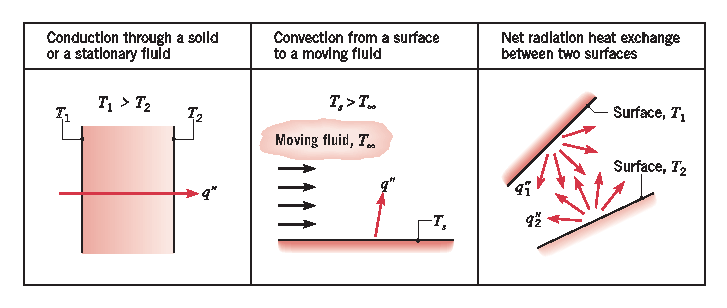
\includegraphics[width = 0.9\textwidth]{img/modes_of_heat_transport.eps}
    \caption{Conduction, convection, and radiation heat transfer modes}
\end{figure}

\subsection{Conduction}
\begin{itemize}
    \item Heat Transport between molecules \textit{via} random collisions. 
    \begin{figure}[H]
        \centering
        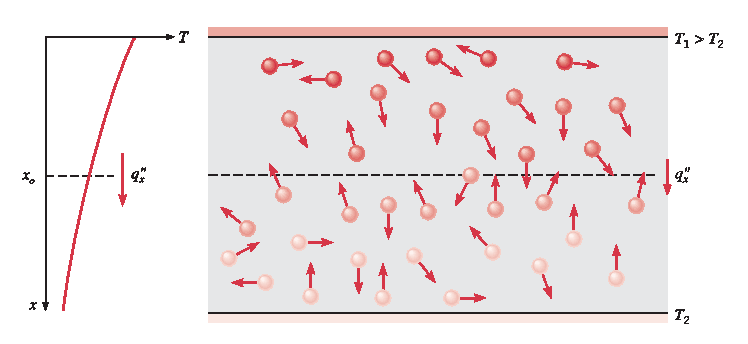
\includegraphics[width = 0.7\textwidth]{img/conduction.eps}
        \caption{Association of conduction heat transfer with diffusion of energy due to molecular activity.}
    \end{figure}
    
    Consider conduction within a gas under a temperature gradient where no bulk motion occurs. The energy is transferred from the high-energy molecules to the low-energy molecules by collision.

\item In 1-D, heat conduction is governed by \textbf{Fourier's Law:} 
\[
    \dot{Q} = -k \ A \ \frac{\mathrm{d}T}{\mathrm{d}x}
\] 


\begin{itemize}
    \item[-] $k$: thermal conductivity  ${\color{gray}\mathrm{[W/(m \cdot K)]}}$: an intrinsic property of material - how good the material is to conduct heat?

    \item[-] $A$: surface area ${\color{gray}\mathrm{[m^2]}}$
    
    \item[-] $\frac{\mathrm{d}T}{\mathrm{d}x}$: temperature gradient in $x$-direction ${\color{gray}\mathrm{[K/m]}}$
\end{itemize}
\end{itemize}

  
\subsection{Convection}
\begin{itemize}
    \item Heat transport due to bulk motion over a heated surface. It occurs at an interface between a fluid in motion and a bounding surface when the two are at different temperatures.

    \begin{figure}[H]
        \centering
        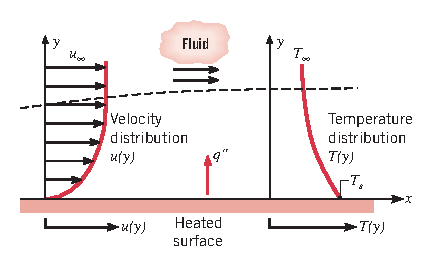
\includegraphics[width = 0.6\textwidth]{img/convection.eps}
        \caption{Boundary layer development in convection heat transfer.}
    \end{figure}

    \item Convective heat flux is described by \textbf{Newton’s law of cooling:}
    \[ 
        \dot{Q} = h \ A \ (T_{s} - T_{\infty}) 
    \]
    
    \begin{itemize}
        \item[-] $h$: convective heat transport coefficient $\color{gray}{\mathrm{[W/(m^{2}\cdot K)]}}$
        \begin{itemize}
            \item highly sensitive to flow patterns, geometry, transport properties
            \item difficult to compute, but some analytical and tabulated values exist
        \end{itemize}
    \end{itemize}

    \item Two types of convective heat transport:
    \begin{itemize}
        \item \textbf{Forced convection:} fluid motion is determined by the external source.
        \item \textbf{Free Convection:} fluid motion is determined by temperature differences and buoyancy forces.
    \begin{figure}[H]
        \centering
        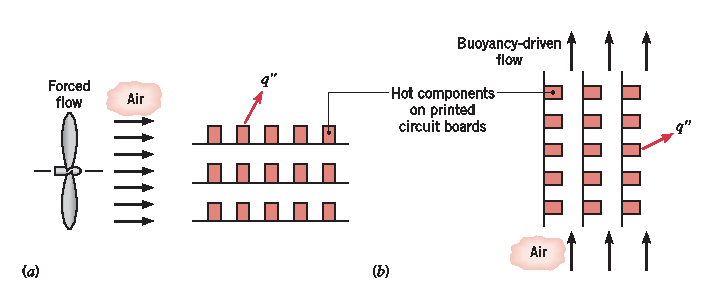
\includegraphics[width = 0.8\textwidth]{img/forced_and_free_convection.eps}
        \caption{(a) Forced convection, (b) Free convection}
    \end{figure}

    \item Mixed convection: convection influenced by both the external source and buoyancy
    \end{itemize}
\end{itemize}
 
\subsection{Radiation}
\begin{itemize}
    \item In radiation, heat transport is due to the propagation of electromagnetic waves (photons). It occurs at any finite temperature for solid, liquid or gas, and does not require physical contact or material medium (efficient in vacuum).
    
    \item Black body radiation, $E_{b}$, is described by Stefan-Boltzmann law: 
    \[ E_{b} = \sigma \ T^{4} \] 
    where $\sigma$ is the Stefan-Boltzmann constant with its value $ 5.67\times10^{-8} \mathrm{W/(m^{2} K^{4})}$

    \item However, real materials are not ideal black bodies:  \[ E = \epsilon \ \sigma \ T^{4} \] where $\epsilon$ is the emissivity with its value $0 \leq \epsilon \leq 1$

    \item Radiation also incident on the surface from surroundings (irradiation or $G$). But only a portion of $G$ is absorbed, rest is reflected or transmitted. This can be described by \[ G_{abs} = \alpha  \ G \] where $\alpha$ is absorptivity with its value $0 \leq \alpha \leq 1$
\end{itemize}

% \newpage
% \section{Control Volumes}
% \subsection{Conservation Laws}
% \[
%     \underbrace{\mathrm{d}U}_{\text{\ding{192}}} = \underbrace{\delta Q}_{\text{\ding{193}}} - \underbrace{\delta W}_{\text{\ding{194}}} + \underbrace{\mathrm{d}S}_{\text{\ding{195}}}
% \]
% \begin{center}
% \begin{tabular}{llll}
%     \text{\ding{192}} & Increase in energy & \text{\ding{193}} & Amount of inflow \\
%     \text{\ding{194}} & Amount of outflow &
%     \text{\ding{195}} & Amount of generation \\
% \end{tabular}
% \end{center}
% Written in terms of \textit{rate of change}:
% \[ 
%     \frac{\mathrm{d}U}{\mathrm{d}t} = \frac{\partial Q}{\partial t} - \frac{\partial W}{\partial t} +\frac{\partial S}{\partial t} =\dot{Q} - \dot{W} +\dot{S} 
% \]


% \subsection{Control Volume}
% \paragraph{Control volume (CV)} is a defined \underline{region of space} where a conservation law is applied.
% \begin{itemize}
%     \item[-] can be any shape and size - chosen based on convenience;
%     \item[-] must be used consistently throughout the problem;
% \end{itemize}

 % \begin{itemize}
 % \item \textbf{Control Volume (CV)}: A defined \underline{region of space} where a conservation law is applied. 
 %   \begin{itemize}
 %   \item A CV can be any shape or size, chosen often based on convenience, but must be used consistently throughout the problem. 
 %   \item CVs may be open or closed, stationary or moving.
 %   \end{itemize}
 %  \item \textbf{Control Surface:} The surface of a CV, through which heat or mass may pass to enter the CV.
 %  \item \textbf{Open CV: } A CV where there is fluid flow (in addition to heat flow) across the control surface. Fluid flow may carry internal, kinetic or potential energy.
 %  \item \textbf{Closed CV:} A CV where there is heat flow (but no fluid flow) across the control surface. All energy Transport is due to work or heat Transport.
 %  \item \textbf{System:} A fixed, identifiable \underline{collection of matter} (sometimes called a control mass). A system often coincides with a control volume, but this is not always the case. Distinction is important, particularly for open CVs.
 %  \end{itemize}


\newpage
\section{Reynolds Transport Theorem}
\subsection{Conservation Laws}
\[
    \underbrace{\mathrm{d}U}_{\text{\ding{192}}} = \underbrace{\delta Q}_{\text{\ding{193}}} - \underbrace{\delta W}_{\text{\ding{194}}} + \underbrace{\mathrm{d}S}_{\text{\ding{195}}}
\]
\begin{center}
\begin{tabular}{llll}
    \text{\ding{192}} & Increase in energy & \text{\ding{193}} & Amount of inflow \\
    \text{\ding{194}} & Amount of outflow &
    \text{\ding{195}} & Amount of generation \\
\end{tabular}
\end{center}
Written in terms of \textit{rate of change}:
\[ 
    \frac{\mathrm{d}U}{\mathrm{d}t} = \frac{\partial Q}{\partial t} - \frac{\partial W}{\partial t} +\frac{\partial S}{\partial t} =\dot{Q} - \dot{W} +\dot{S} 
\]


\subsection{Control Volume}
\paragraph{Control Volume (CV)} is a defined \underline{region of space} where a conservation law is applied.
\begin{itemize}
    \item[-] can be any shape and size - chosen based on convenience;
    \item[-] must be used consistently throughout the problem;
\end{itemize}

\subsection{Kinematics Description and Material Derivative} 
\paragraph{Kinematics} Description of motion of mass in time and space, noting about forces driving that motion. \\

Two general approaches used in kinematics are \textbf{Lagrangian} and \textbf{Eulerian}.

\begin{figure}[H]
    \centering
    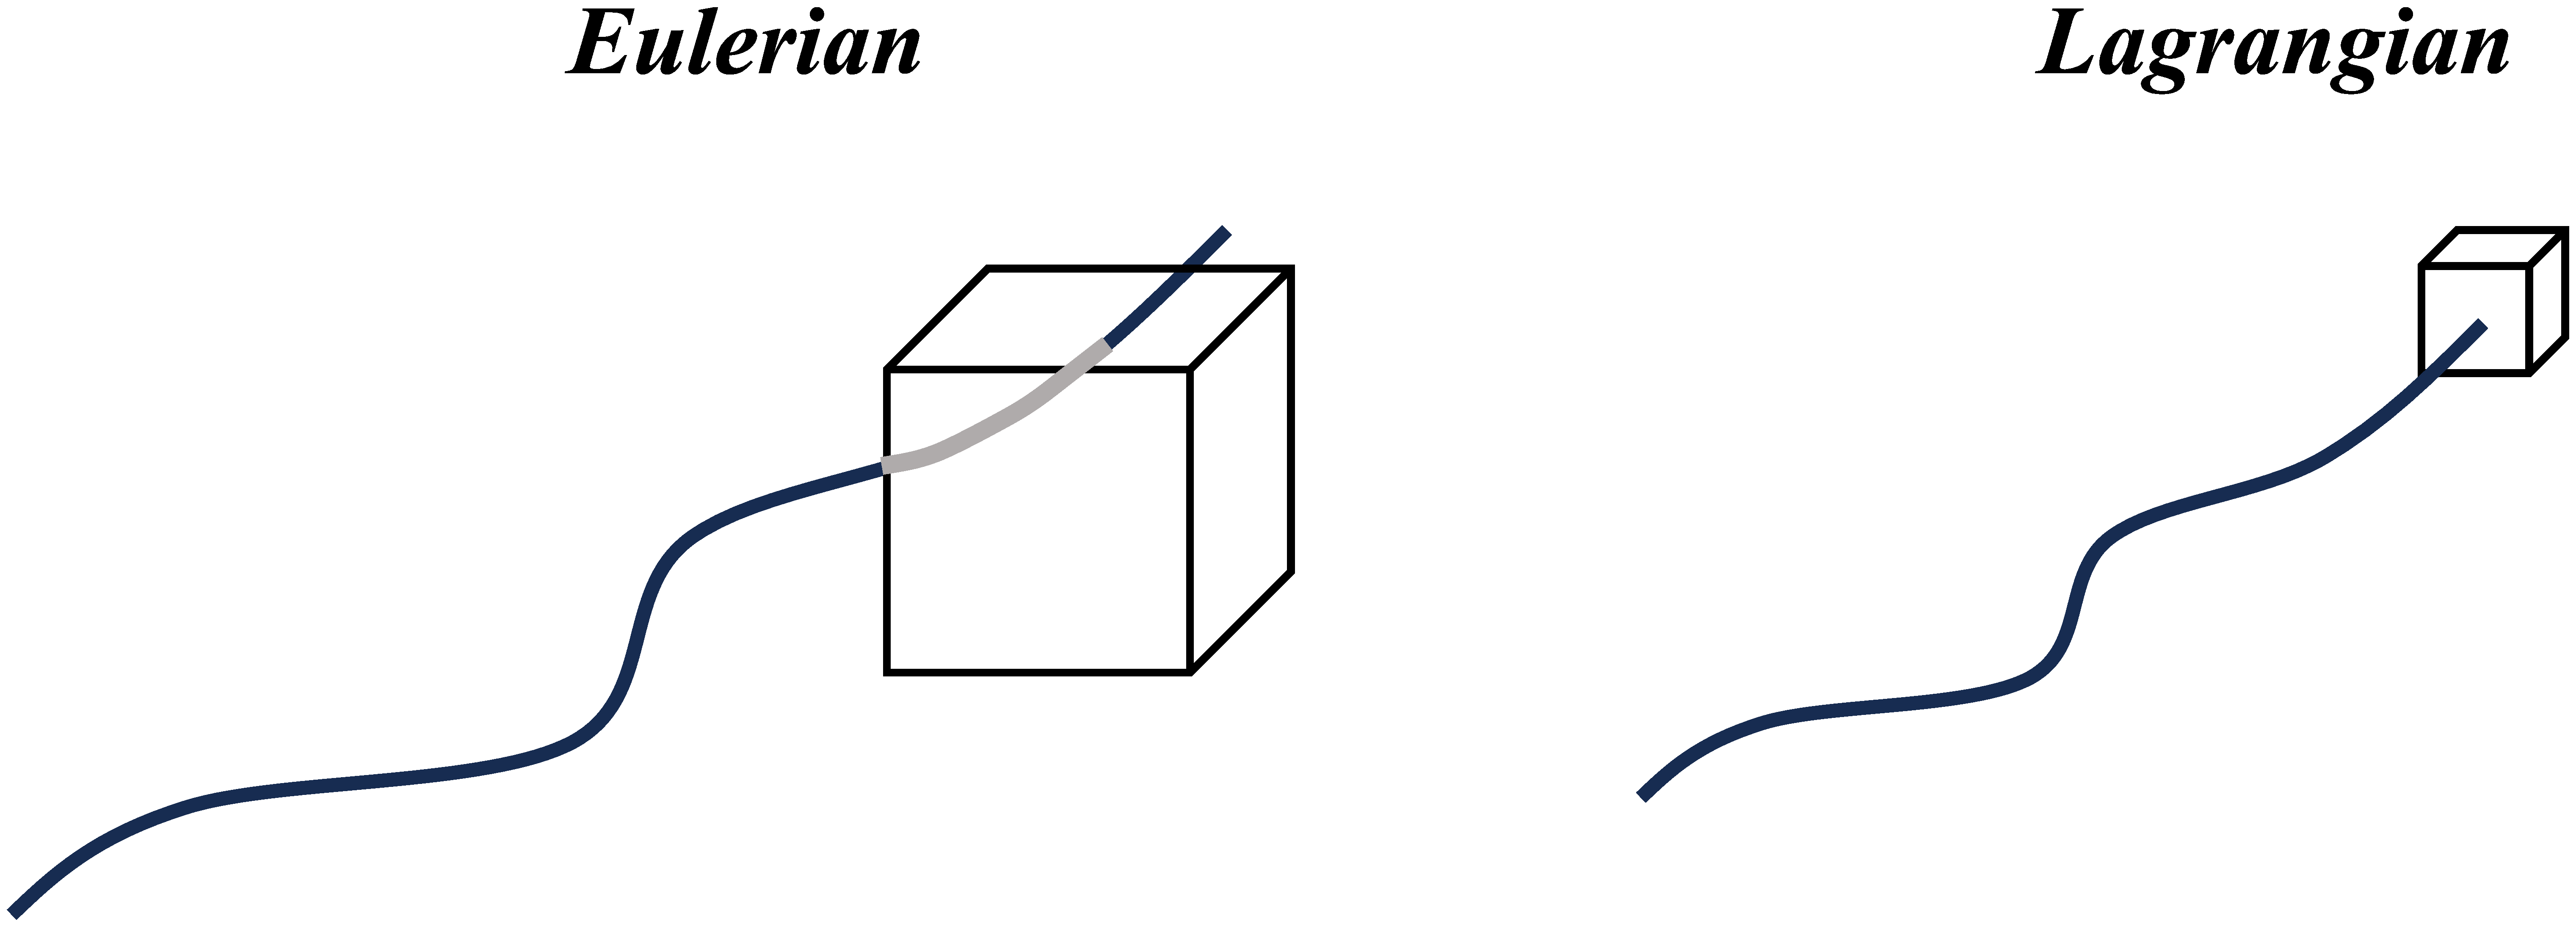
\includegraphics[width=.7\textwidth]{img/lagrangian_eulerian.eps}
    \caption{Eulerian and Lagrangian description of the kinematics.}
\end{figure}

\begin{table}[H]
    \centering
    \begin{tabularx}{\textwidth}{X|X}
         \textbf{Lagrangian} & \textbf{Eulerian} \\ \hline
        \begin{itemize}
           \item keeps track of individual particles as they move through space 
           \item often called "material-following" approach
           \item Difficult in practice
        \end{itemize}
        & 
        \begin{itemize}
            \item describes particle velocity as a function of space
            \item Convenient in mathematical approach, but leads to some paradoxes
        \end{itemize} 
    \end{tabularx}
\end{table}

\paragraph{Material Derivative} links the Eulerian and Lagrangian reference frames.
\[ 
    \frac{Dg}{Dt} = \frac{\partial g}{\partial t}+ (\bm{v} \cdot \nabla)g 
\]
 
\begin{tcolorbox}[breakable, title=\textbf{Derivation}] 
Let $g(\bm{x}, t) = g(x, y, z, t)$ be an arbitrary property of a mass particle defined in an Eulerian field. As the particle moves through the field, the property assumes the local value of $g(\bm{x}, t)$. \textbf{What is the rate of change of $g(\bm{x}, t)$?}
\begin{align*} 
\begin{split}
\frac{Dg}{Dt} 
& =\frac{\mathrm{d}}{\mathrm{d}t}g(\overbrace{X(t),Y(t),Z(t)}^{\bm{X}(t)},t) \\
& = \frac{\partial g}{\partial x} \cancelto{v_{x}}{\frac{\mathrm{d}X}{\mathrm{d}t}} + \frac{\partial g}{\partial y} \cancelto{v_{y}}{\frac{\mathrm{d}Y}{\mathrm{d}t}} + \frac{\partial g}{\partial z} \cancelto{v_{z}}{\frac{\mathrm{d}Z}{\mathrm{d}t}} + \frac{\partial g}{\partial t}\\\\
& = v_{x}\frac{\partial g}{\partial x} + v_{y}\frac{\partial g}{\partial y} + v_{z}\frac{\partial g}{\partial z} + \frac{\partial g}{\partial t}\\
& = \underbrace{\frac{\partial g}{\partial t}}_{\text{unsteady}} + \underbrace{(\bm{v} \cdot \nabla)g}_{\text{advection}}
\end{split} 
\end{align*}
where the vector $\bm{v} \in [v_x, v_y, v_z]$.
\end{tcolorbox}

%========================================
\subsection{Flow and Flux}
\subsubsection{Flow}
\paragraph{Flow} Flow quantifies how much of a substance or property is being transported across a surface per unit of time. \textbf{Flow is an \emph{extensive} property.}

\begin{tcolorbox}[breakable, title = \textbf{Typical Units of Flows}]
    \begin{itemize}
        \item flux of solute: $\displaystyle \mathrm{M/s}$
        \item flux of heat: $\displaystyle \mathrm{J/s = W}$
        \item flux of solvent: $\displaystyle \mathrm{m^{3}/s}$
    \end{itemize}
\end{tcolorbox}

\paragraph{Extensive Property} is a physical property that depends on the size or the amount of material contained in system. It cannot be defined at a point.
\begin{itemize}
 \item Examples: mass, energy, momentum
\end{itemize}


\subsubsection{Flux}
\paragraph{Flux} Flux quantifies how much of a substance or property is being transported across a surface per unit of time and per unit area. \textbf{Flux is an \emph{intensive} property.}

\begin{tcolorbox}[breakable, title = \textbf{Typical Units of Fluxes}]
    \begin{itemize}
        \item flux of solute: $\displaystyle \mathrm{M/(m^{2}s)}$
        \item flux of heat: $\displaystyle \mathrm{J/(m^{2}s) = W/(m^{2})}$
        \item flux of solvent: $\displaystyle \mathrm{m^{3}/(m^{2}s) = m/s}$
    \end{itemize}
\end{tcolorbox}

\paragraph{Intensive Property} is independent of size or the amount of material contained in the system. It cannot be defined at each point (per unit volume, unit area, unit mass);
\begin{itemize}
    \item Examples: density, concentration.
\end{itemize}

Integrating an intensive property over space containing mass translates an intensive property into an extensive property.


\subsubsection{Flux Orientation and Volume Flow Rate}
Flow across a surface depends on the relative orientation between flux and surface.
\begin{figure}[H]
    \centering
    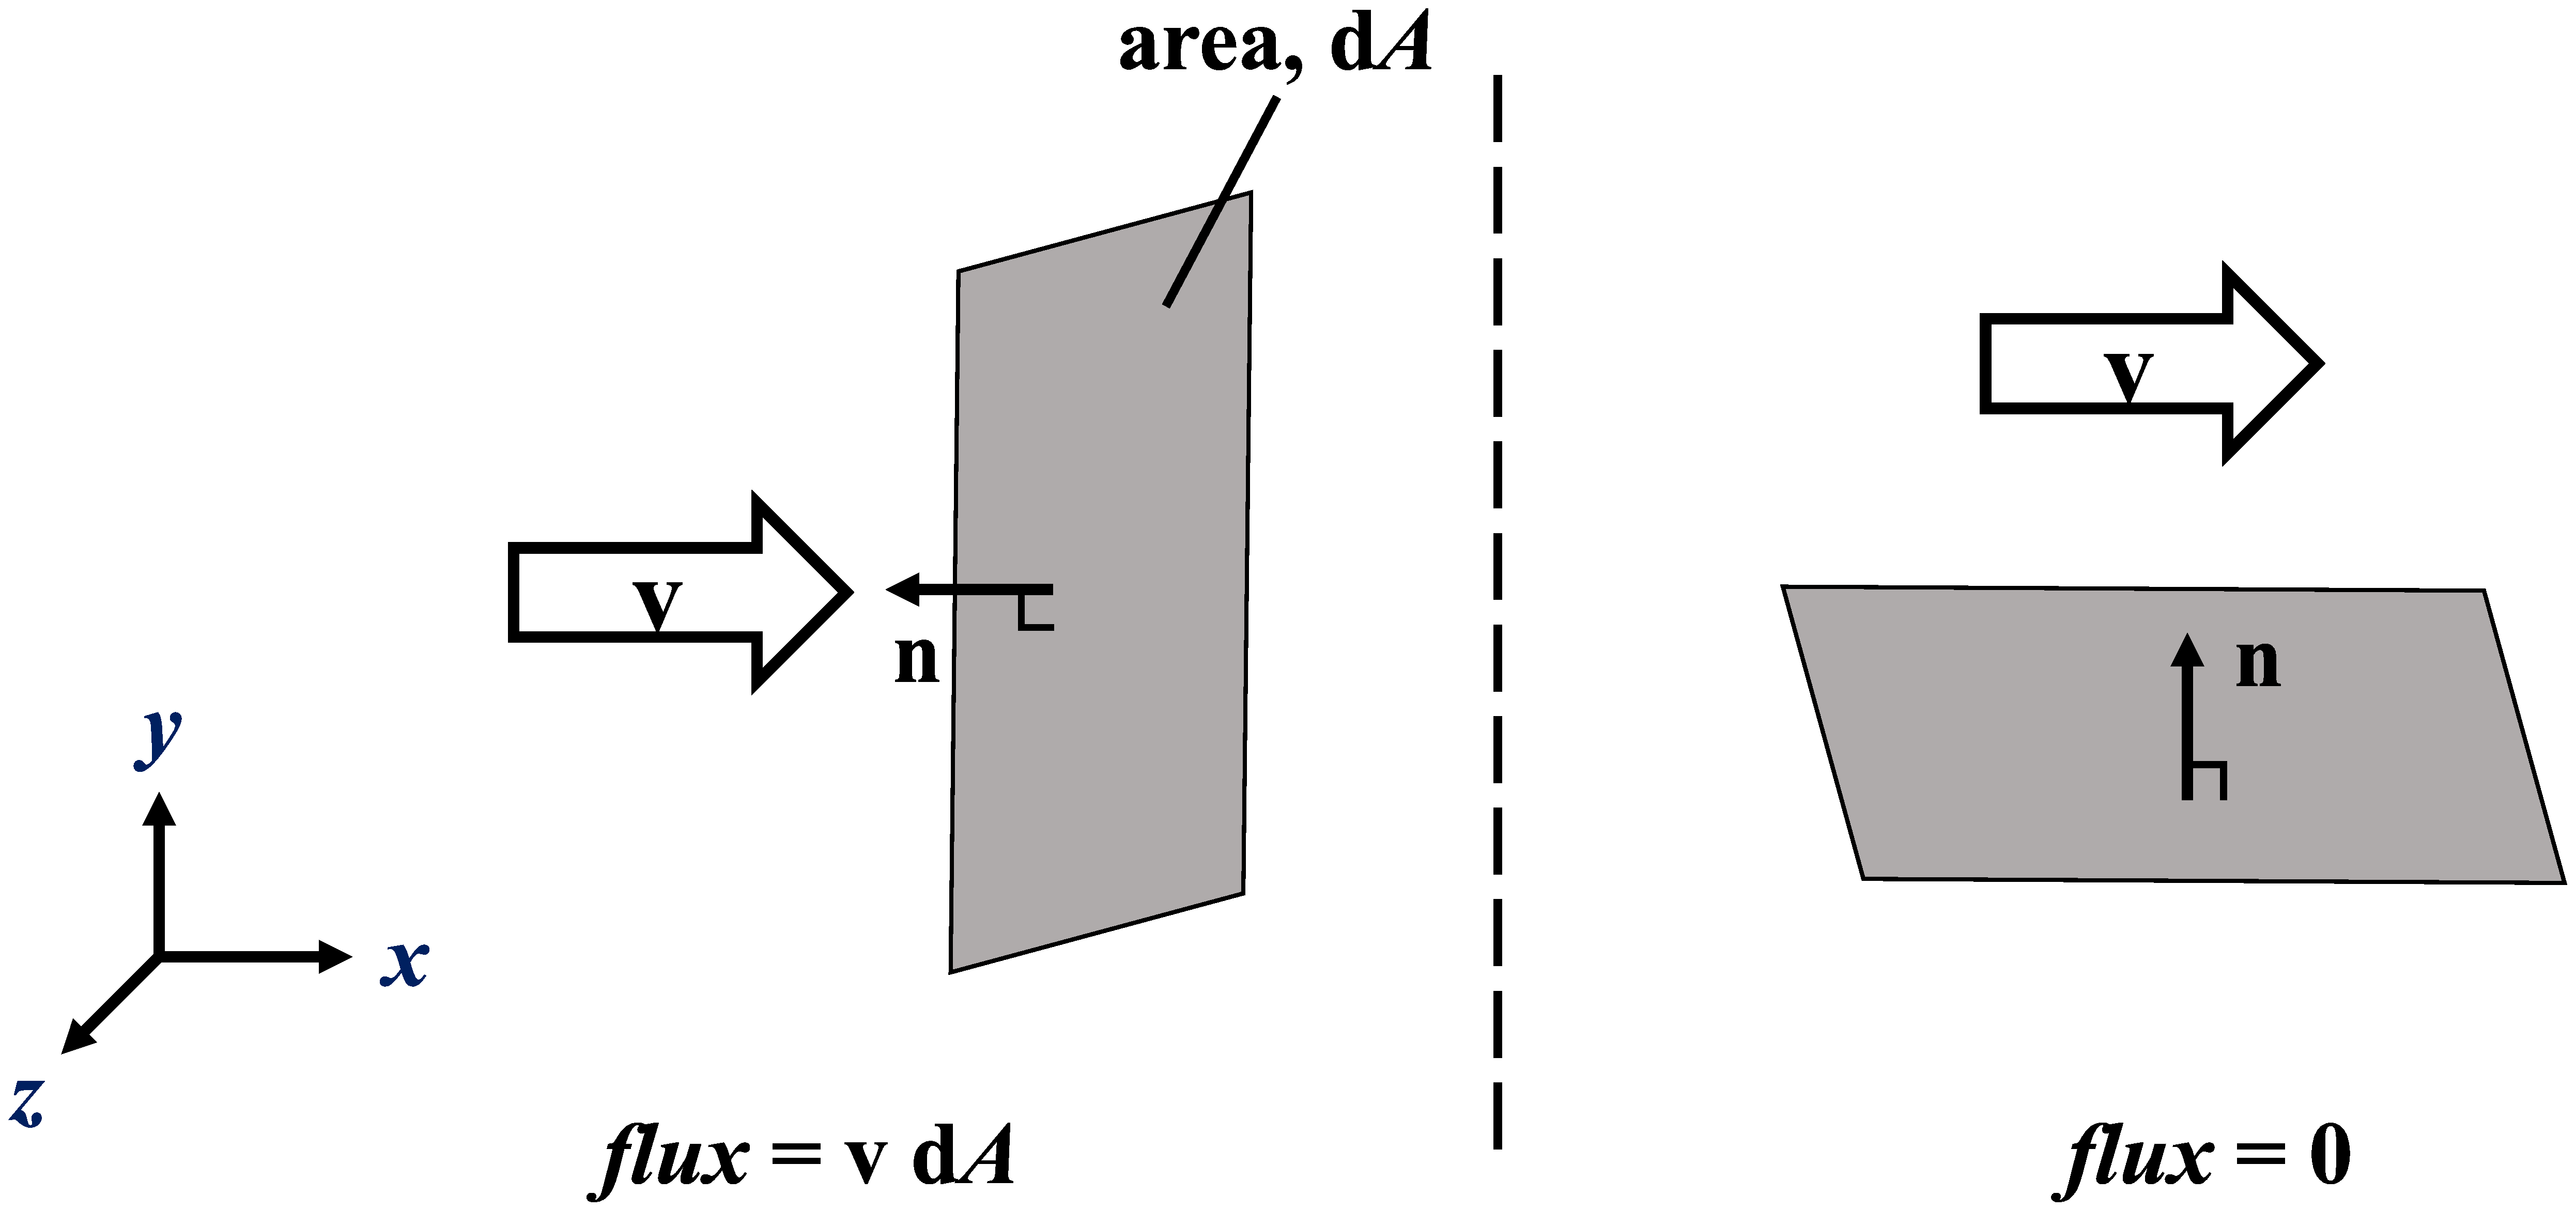
\includegraphics[width=.7\textwidth]{img/flux_orientation.eps}
\end{figure}
Mathematically, the \textbf{intensive volume flow rate} is
\[ 
    \mathrm{d}V=(\bm{v} \cdot \bm{\hat{n}}) \ \mathrm{d}A \ \mathrm{d}t \quad or \quad \frac{\mathrm{d}V}{\mathrm{d}t}=(\bm{v} \cdot \bm{\hat{n}}) \ \mathrm{d}A 
\]
where
\begin{itemize}
    \item[-] $\bm{\hat{n}}$ represents the outward facing normal or a control surface: $\bm{\hat{n}}=n_{x}\hat{e}_{x}+n_{y}\hat{e}_{y}+n_{z}\hat{e}_{z}$.
    \item[-] $\bm{v}$ represents the velocity of flux crossing the surface: $\bm{v}=v_{x}\hat{e}_{x}+v_{y}\hat{e}_{y}+v_{z}\hat{e}_{z}$.
\end{itemize}

% where $\mathrm{d}V$ denotes the small volume of fluid leaving CV.
\textbf{Extensive flow rate:}
\[ 
    Q = \int_{A} (\bm{v} \cdot \bm{\hat{n}}) \ \mathrm{d}A 
\]


\textbf{Generalize} to any arbitrary extensive property $B$, where $\beta = \frac{\mathrm{d}B}{\mathrm{d}m}$, total rate of transport of $B$ across surface area $A$ due to fluid flow is:
\[
    Q =  \int_{A} \rho \beta (\bm{v} \cdot \bm{n}) \ \mathrm{d}A 
\]

\subsection{Reynolds Transport Theorem (RTT)}
\begin{equation}
\label{eqn:RTT}
    \frac{\mathrm{d}B_{system}}{\mathrm{d}t} 
    = \frac{\partial}{\partial t} \int\limits_{CV} \rho \beta \mathrm{d}V 
    + \oint\limits_{CS} \rho \beta (\bm{v} \cdot \bm{\hat{n}})\mathrm{d}A 
\end{equation}

\begin{tcolorbox}[breakable, title = Derivation]
\begin{figure}[H]
    \centering
    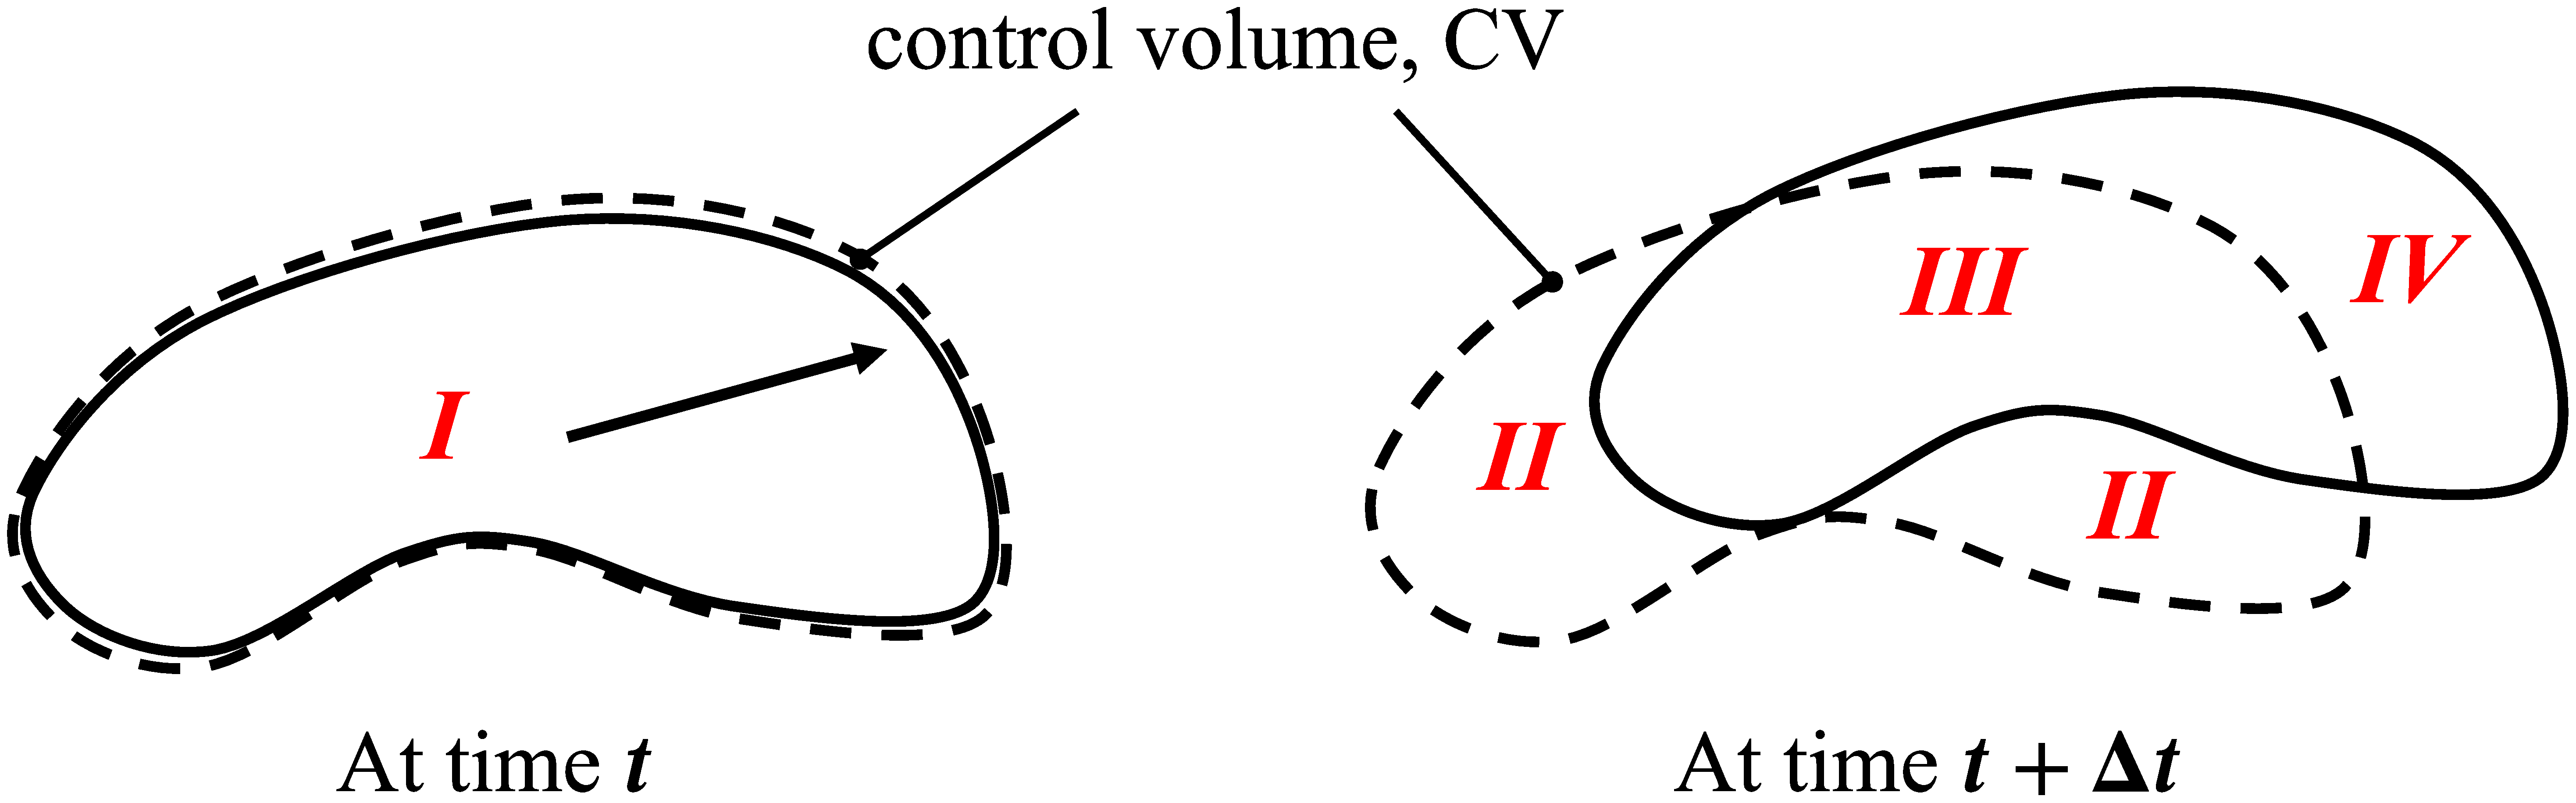
\includegraphics[width = 0.9\textwidth]{img/control_volume.eps}
\end{figure}

\begin{itemize}
    \item[-] \textbf{I}  entire fluid system within CV at time $t$
    \item[-] \textbf{II} new fluid that has entered CV at time $t + \Delta t$
    \item[-] \textbf{III} portion of fluid system that remains inside CV at time $t + \Delta t$
    \item[-] \textbf{IV} portion of fluid system that is outside of CV at time $t + \Delta t$
\end{itemize}

By conservation of mass: \textit{``how much out equals to how much in''}
\begin{align*}
\begin{split}
    \underbrace{B_{system} \lvert_{t + \Delta t}  \ -\  B_{system} \lvert_{t}}_{\text{change of B in system}} & = B_{III}+B_{IV}-B_{I}\\
    & = \underbrace{(B_{III}+B_{II}-B_{I})}_{\text{change of B in CV}}\quad +\underbrace{(B_{IV}-B_{II})}_{\substack{\text{Net amount of B} \\ \text{leaving CV due to flow}}}\\
\end{split}
\end{align*}

\begin{align*}
\begin{split}
    \underbrace{B_{system} \lvert_{t + \Delta t} \ -\ B_{system}}_{\textbf{Term A}} 
    &= \underbrace{B_{CV} \lvert_{t + \Delta t} \ -\  B_{CV}  \lvert_{t}}_{\textbf{Term B}}\\
    & + \underbrace{\text{Net amount of B leaving CV due to flow}}_{\textbf{Term C}}
\end{split}
\end{align*}

 Divide each term by $\Delta t$, and take limit as $t \to 0$\\
\\ \textbf{Term A}: rate of change of B within system (Lagrangian)
 \[ 
 \lim_{\Delta t \to 0}\frac{B_{system} \lvert_{t + \Delta t} \ -\ B_{system}}{\Delta t} = \frac{\mathrm{d}B_{system}}{\mathrm{d}t} 
 \]
\\ 
\textbf{Term B}: rate of change of B within CV (Eulerian)
\[ 
 \lim_{\Delta t \to 0} \frac{B_{CV} \lvert_{t + \Delta t} \ -\  B_{CV}  \lvert_{t}}{\Delta t} = \frac{\partial B_{CV}}{\partial t} = \frac{\partial}{\partial t} \int\limits_{CV} \rho \beta \mathrm{d}V
\]
 \\ 
\textbf{Term C}: rate of change of B within CV as it is lost by fluid flow (Eulerian)
\begin{align*} 
\begin{split}
    \lim_{\Delta t \to 0} \frac{\text{Net amount of B leaving CV due to flow}}{\Delta t} \\
    & = \text{rate of B leaving CV due to flow}\\
    & = \oint\limits_{CS} \rho \beta (\bm{v} \cdot \bm{\hat{n}})\mathrm{d}A 
\end{split}
\end{align*}

To equate these three terms,
\[
    \textbf{term A} = \textbf{Term B} + \textbf{Term B}
    \quad \Rightarrow \quad
    \frac{\mathrm{d}B_{system}}{\mathrm{d}t} 
    = \frac{\partial}{\partial t} \int\limits_{CV} \rho \beta \mathrm{d}V 
    + \oint\limits_{CS} \rho \beta (\bm{v} \cdot \bm{n})\mathrm{d}A 
\]
which states the RTT expressed in \autoref{eqn:RTT}.
\end{tcolorbox}


\newpage
\section{Heat Equation}
\subsection{Integral Form of Heat Equation}
When $B \to U, \quad \beta \to U_{M}$, RTT can be expressed as
\[
    \frac{\mathrm{d}U_{system}}{\mathrm{d}t} = \frac{\partial}{\partial t} \int\limits_{CV} \rho U_{M} \ \mathrm{d}V +  \oint\limits_{CS} \rho U_{M} (\bm{v} \cdot \bm{\hat{n}}) \ \mathrm{d}A
\]
The rate of change of the system, $\frac{\mathrm{d}U_{system}}{\mathrm{d}t}$ can be further expand with the expression $\dot{Q}-\dot{W}+\dot{S}$,
\[
  \dot{Q}-\dot{W}+\dot{S} = \frac{\partial}{\partial t} \int\limits_{CV} \rho U_{M} \ \mathrm{d}V +  \oint\limits_{CS} \rho U_{M} (\bm{v} \cdot \bm{\hat{n}}) \ \mathrm{d}A
\]

By applying the following constraints and rearranging the expressions,
\begin{enumerate}
    \item Only the thermal energy is considered: $\rho U_{M} = \rho c_{p} T$, where $c_{p}$ is specific heat at constant pressure [J/kg K],
    \[
        \dot{Q}-\dot{W}+\dot{S} = \frac{\partial}{\partial t} \int\limits_{CV} \rho c_p T \ \mathrm{d}V +  \oint\limits_{CS} \rho c_p T (\bm{v} \cdot \bm{\hat{n}}) \ \mathrm{d}A
    \]
    
    \item \begin{itemize}
        \item[-] $\dot{Q}$ is the rate of heat transport into CV through CS: $\displaystyle \dot{Q} = -\oint\limits_{CS}(\bm{q} \cdot \bm{\hat{n}}) \mathrm{d}A$, where $\bm{q}$ is the heat flux vector;
        \item[-] neglect contributions of work terms: $\dot{W}=0$;
        \item[-] heat generation per unit volume: $\displaystyle \dot{S_{v}}: \dot{S} = \int\limits_{CV}\dot{S_{v}} \mathrm{d}V$.
    \end{itemize}
    \[
        -\oint\limits_{CS}(\bm{q} \cdot \bm{\hat{n}}) \mathrm{d}A+\dot{S}_v = \frac{\partial}{\partial t} \int\limits_{CV} \rho c_p T \ \mathrm{d}V +  \oint\limits_{CS} \rho c_p T (\bm{v} \cdot \bm{n}) \ \mathrm{d}A
    \]
\end{enumerate}

Re-arrange the above expression, this gives us the final expression of \textbf{conservation of mass}.
\begin{equation}
\label{eqn:mass_conserve}
    \boxed{ 
    \underbrace{\frac{\partial}{\partial t} \int\limits_{CV} \rho c_{p} \mathrm{d}V}_{\substack{\text{rate of change}\\\text{of thermal energy}}} 
    = \underbrace{\int\limits_{CV} \dot{S_{v}} \mathrm{d}V}_{\text{rate of heat generation}} 
    - \underbrace{\oint\limits_{CS} (\bm{q} \cdot \bm{\hat{n}}) \mathrm{d}A}_{\substack{\text{rate of heat loss}\\\text{due to heat flux}}} 
    - \underbrace{\oint\limits_{CS} \rho c_{p} T (\bm{v} \cdot \bm{\hat{n}}) \mathrm{d}A}_{\substack{\text{rate of heat loss}\\ \text{by fluid flow across CS}}} 
}
\end{equation}
 
 
\subsection{An Example}
\begin{tcolorbox}[breakable, title = Example: Cooling of a Circuit Board]
\begin{figure}[H]
    \centering
    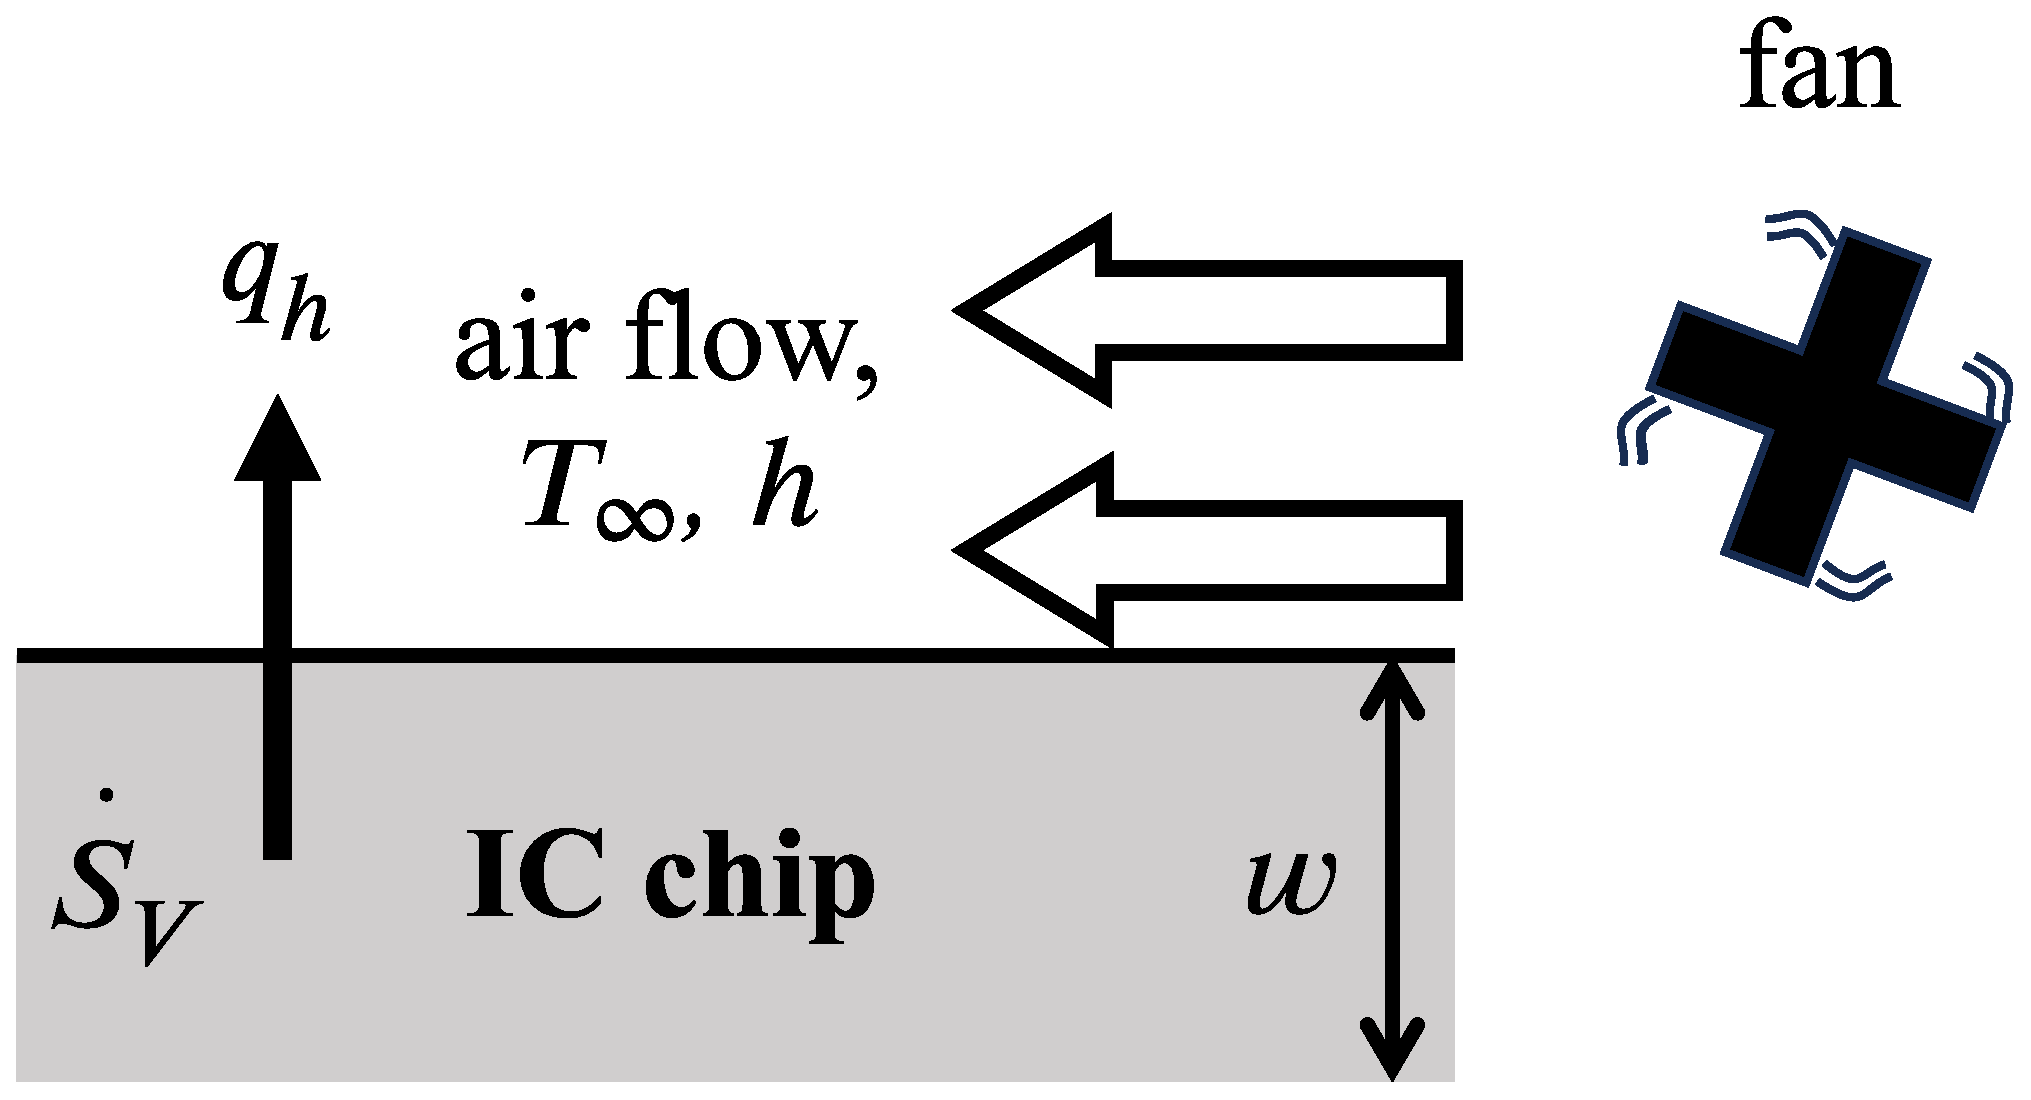
\includegraphics[width=0.5\textwidth]{img/cooling_fan.eps}
\end{figure}
\paragraph{Problem Description} An integrated circuit chip generates heat during operation at a constant rate $\dot{S_{v}}$ in units of $W/m^{3}$. Forced convection from a fan is used to cool the chip during operation. The temperature of air from the fan is $T_{\infty}$, with convective heat transport $h$. The surface area of the chip is $A$. The chip is insulated on all sides except the top. The thickness of the chip is $w$. Assume that the IC chip has uniform internal temperature.

\paragraph{Aim} Find an expression for the steady-state temperature, $T_s$, of the IC chip.
%Need graphs for CV
\paragraph{Solution Procedure} Start from the heat equation:
\[ 
    \cancelto{0, \text{steady-state}}{\frac{\partial}{\partial t} \int\limits_{CV} \rho c_{p} T \mathrm{d}V} = \int\limits_{CV} \dot{S_{v}} \mathrm{d}V - \oint\limits_{CS} (\bm{q} \cdot \bm{\hat{n}}) \mathrm{d}A - \cancelto{0,\text{no advection}}{\oint\limits_{CS} \rho c_{p} T (\bm{v} \cdot \bm{n}) \mathrm{d}A}
\]
which is eliminated to
\[ 
    \underbrace{\int\limits_{CV} \dot{S_{v}} \mathrm{d}V}_{= \dot{S_{v}} V = \dot{S_{v}} w A}
    = \underbrace{\oint\limits_{CS} (\bm{q} \cdot \bm{\hat{n}}) \mathrm{d}A}_{= q_{h} A = h(T_{s}-T_{\infty}) A}
\]
Therefore, to equate L.H.S and R.H.S.,
\[ 
    \dot{S_{v}} w A = h(T_{s}-T_{\infty}) A \ \Rightarrow \  \boxed{T_{s} = \frac{\dot{S_{v}} w}{h}+T_{\infty}} 
\]
Checking units: 
$[\mathrm{K}] (\text{L.H.S.}) = \bigg[ \frac{\mathrm{W}}{\mathrm{m}^{3}} \cdot \frac{\mathrm{m}}{\mathrm{W}/\mathrm{Km}^{2}} \bigg] = [\mathrm{K}] (\text{R.H.S.}) \ \Rightarrow \ \checkmark$
\end{tcolorbox}

\subsection{Differential Form of Heat Equation}
\subsubsection{Divergence Theorem}
\begin{itemize}
    \item The \textbf{Divergence Theorem} (Gauss' Theorem) states that \textbf{the net quantity of any vector leaving a volume} is equal to \textbf{net flow of that vector across the surface bounding that volume}.
    \[ 
        \oint\limits_{CS}(\bm{f} \cdot \hat{n}) \ \mathrm{d}A = \int\limits_{CV} (\nabla \cdot \bm{f}) \ \mathrm{d}V 
    \]
    
    \item The divergence theorem transforms a \textbf{surface} integral into a \textbf{volume} integral.
    \begin{itemize}
        \item[-] $\bm{f}$ can be any arbitrary vector
        \item[-] $\nabla \cdot$ is the divergence operator, where $\nabla \cdot \bm{f} = \frac{\partial f_{x}}{\partial x}+\frac{\partial f_{y}}{\partial y}+\frac{\partial f_{z}}{\partial z}$
    \end{itemize}
\end{itemize}


\subsubsection{Differential Form of Heat Equation}
\[ 
    \rho c_{p}\bigg( \underbrace{\frac{\partial T}{\partial t}}_{\text{\ding{192}}} + \underbrace{(\bm{v} \cdot \nabla) T}_{\text{\ding{193}}} \bigg) = \underbrace{\dot{S_{v}}}_{\text{\ding{194}}} + \underbrace{k\nabla^{2}T}_{\text{\ding{195}}} 
\]
\begin{center}
\begin{tabular}{llll}
    \text{\ding{192}} & unsteady term & \text{\ding{193}} & convective term \\
    \text{\ding{194}} & source term & \text{\ding{195}} & diffusive term
\end{tabular}
\end{center}


\begin{tcolorbox}[breakable, title = \textbf{Derivation}]
Apply the divergence theorem into heat equation:
\[ 
    \oint\limits_{CS} (\bm{q} \cdot \bm{\hat{n}}) \mathrm{d}A = \int\limits_{CV} (\nabla \cdot \bm{q}) \mathrm{d}V
\]
\[ 
    \oint\limits_{CS} \rho c_{p} T (\bm{v} \cdot \hat{n}) \mathrm{d}A =  \int\limits_{CV} (\nabla \cdot (\rho c_{p} T \bm{v})) \mathrm{d}V 
\]
Therefore,
\begin{align*}
\begin{split}
    \frac{\partial}{\partial t} \int\limits_{CV} \rho c_{p} T \mathrm{d}V 
    &= \int\limits_{CV} \dot{S_{v}} \mathrm{d}V - \oint\limits_{CS} (\bm{q} \cdot \hat{n}) \mathrm{d}A - \oint\limits_{CS} \rho c_{p} T (\bm{v} \cdot \hat{n}) \mathrm{d}A \\
    &= \int\limits_{CV} \dot{S_{v}} \mathrm{d}V - \int\limits_{CV} (\nabla \cdot \bm{q}) \mathrm{d}V - \int\limits_{CV} (\nabla \cdot (\rho c_{p} T \bm{v})) \mathrm{d}V 
\end{split}
\end{align*}
Rearrange:
\[ 
    \int \underbrace{\bigg[ \frac{\partial}{\partial t}\rho c_{p} T - \dot{S_{v}} + (\nabla \cdot \bm{q}) + (\nabla \cdot (\rho c_{p} T \bm{v})) \bigg]}_{0} \mathrm{d}V = 0 
\]
Since:
\begin{itemize}
    \item $\frac{\partial}{\partial t}(\rho c_{p} T) = \rho \frac{\partial (c_{p} T)}{\partial t} +  c_{p} T \frac{\partial  \rho}{\partial t}$
    \item $\nabla \cdot (\rho c_{p} T \bm{v} ) = c_{p} T(\nabla \cdot \rho \bm{v}) + \rho(\bm{v} \ \nabla \cdot c_{p} T) $ 
\end{itemize}
Thus,
\[ 
    \rho \frac{\partial (c_{p} T)}{\partial t} +  c_{p} T \frac{\partial  \rho}{\partial t} = \dot{S_{v}} -(\nabla \cdot \bm{q}) - c_{p} T(\nabla \cdot \rho \bm{v}) - \rho(\bm{v} \ \nabla \cdot c_{p} T) 
\]
Rearrange: assume $c_{p}$ is constant and uniform
\[ 
    \cancelto{0}{c_{p}T \bigg( \frac{\partial  \rho}{\partial t} + \nabla \cdot \rho \bm{v} \bigg)} + \rho c_{p} \bigg(\frac{\partial T}{\partial t} +(\bm{v} \cdot \nabla) T \bigg) = \dot{S_{v}} - (\nabla \cdot \bm{q}) 
\]
Since $\nabla \cdot \bm{q} = -k \nabla^{2} T$.
\paragraph{Result}
\[ 
    \rho c_{p}\bigg( \frac{\partial T}{\partial t} + (\bm{v} \cdot \nabla) T \bigg) = \dot{S_{v}}  +k \nabla^{2} T 
\]
\end{tcolorbox}

\paragraph{Alternatively}
\[ 
    \underbrace{\rho c_{p}\frac{DT}{Dt}}_{\text{\ding{192}}} = \underbrace{\dot{S_{v}}}_{\text{\ding{193}}}  + \underbrace{k \nabla^{2} T}_{\text{\ding{194}}} 
\]
\begin{center}
\begin{tabular}{ll}
    \text{\ding{192}} & Rate of change of heat in fluid particle \\ \text{\ding{193}} & Rate of heat generation \\
    \text{\ding{194}} & Rate of heat accumulation by conduction \\
\end{tabular}
\end{center}

% with the assumptions: no work, radiation, phase change, constant and uniform $c_{p}$, uniform $k$.

\subsubsection{Special Cases of the Differential Form of Heat Equation}

\paragraph{No heat generation ($\dot{S}_{v}=0$)} 
\[ 
    \frac{\partial T}{\partial t} +(\bm{v} \cdot \nabla) T =  \alpha \nabla^{2} T 
\]
where $\displaystyle k \to \alpha=\frac{k}{\rho c_{p}}$ is the \textbf{thermal diffusivity}, with the unit $\mathrm{m}^{2}/\mathrm{s}$.

\paragraph{No advection ($\bm{v}=0$)}
\[ 
    \frac{\partial T}{\partial t} =  \alpha \nabla^{2} T + \frac{\dot{S}_{v}}{\rho c_{p}} 
\]
\paragraph{Steady-state ($\frac{\partial T}{\partial t}=0$)}
\[ 
    (\bm{v} \cdot \nabla) T = \alpha \nabla^{2} T + \frac{\dot{S}_{v}}{\rho c_{p}} 
\]


\subsection{Similarity}
\begin{table}[H]
    \centering
    \begin{tabular}{cccc}
    \toprule
        Transport of ... & Governing Equation & ``Diffusivity'' & Source Term \\
    \midrule
        Heat & $\displaystyle \frac{\partial T}{\partial t} + (\bm{v} \cdot \nabla) T = \alpha \nabla^2 T + \dot{S}_T$ & $\displaystyle \alpha = k/\rho c_p$ & $\dot{S}_{T} = \dot{S}_{v}/\rho c_p$ \\ [.8em]
        Mass & $\displaystyle \frac{\partial C}{\partial t} + (\bm{v} \cdot \nabla) C = D \nabla^2 T + S_C$ & $D$ & $S_{C}$ \\ [.8em]
        Momentum (N-S) & $\displaystyle \frac{\partial \bm{v}}{\partial t} + (\bm{v} \cdot \nabla) \bm{v} = \nu \nabla^2 \bm{v} + \dot{S}_v$ & $\displaystyle \nu = \mu/\rho$ & $\dot{S}_{v} = (-\nabla p + \bm{g})/\rho$ \\
    \bottomrule
    \end{tabular}
\end{table}


\newpage
\section{Steady-State Heat Conduction}
\subsection{Boundary Conditions}
The 1-D heat equation is second-order in spatial coordinates ($x$) and first-order in time ($t$), so two \textit{boundary conditions} and one \textit{initial condition} are needed.
\begin{table}[H]
    \centering
    \begin{tabularx}{\textwidth}{>{\centering\arraybackslash}X|>{\centering\arraybackslash}X|>{\centering\arraybackslash}X}
    \toprule
        \textbf{Dirichlet Condition} & \textbf{Neumann Condition} & \textbf{Newton's Law of Cooling}  \\
    \midrule
        fixed temperature & fixed slope & couples temperature and slope \\
    \centering
    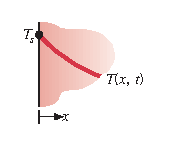
\includegraphics[]{img/Dirichlet.eps} &
    \centering
    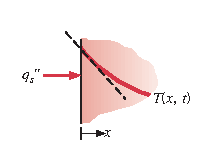
\includegraphics[]{img/Neumann.eps} &
    {\centering
    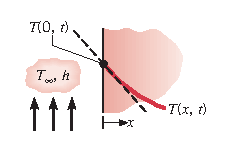
\includegraphics[]{img/Newtons_law_of_cooling.eps}}\\
    \bottomrule
    \end{tabularx}
    \caption{Three types of boundary conditions: Dirichlet, Neumann, Newton's Law of Cooling}
    \label{tab:my_label}
\end{table}
%==========================================================
\subsection{Example 1: 1-D Steady-State Conduction in a Wall}
\begin{tcolorbox}[breakable, title = \textbf{Example: 1-D Steady-State Conduction}]
\begin{minipage}{.6\textwidth}
    \paragraph{Assumptions} 
    \begin{itemize}
        \item 1-D steady-state conduction $\Rightarrow \partial / \partial t = 0$;
        \item no external heat generation $ \Rightarrow \dot{S}_{v} = 0$;
        \item No convection is considered $\Rightarrow (\bm{v} \cdot \nabla) T = 0$;
        \item constant conductivity $k$.
\end{itemize}
\paragraph{Goal} Solve for $T(x)$ in wall.
\end{minipage}
\hfill
\begin{minipage}{.35\textwidth}
    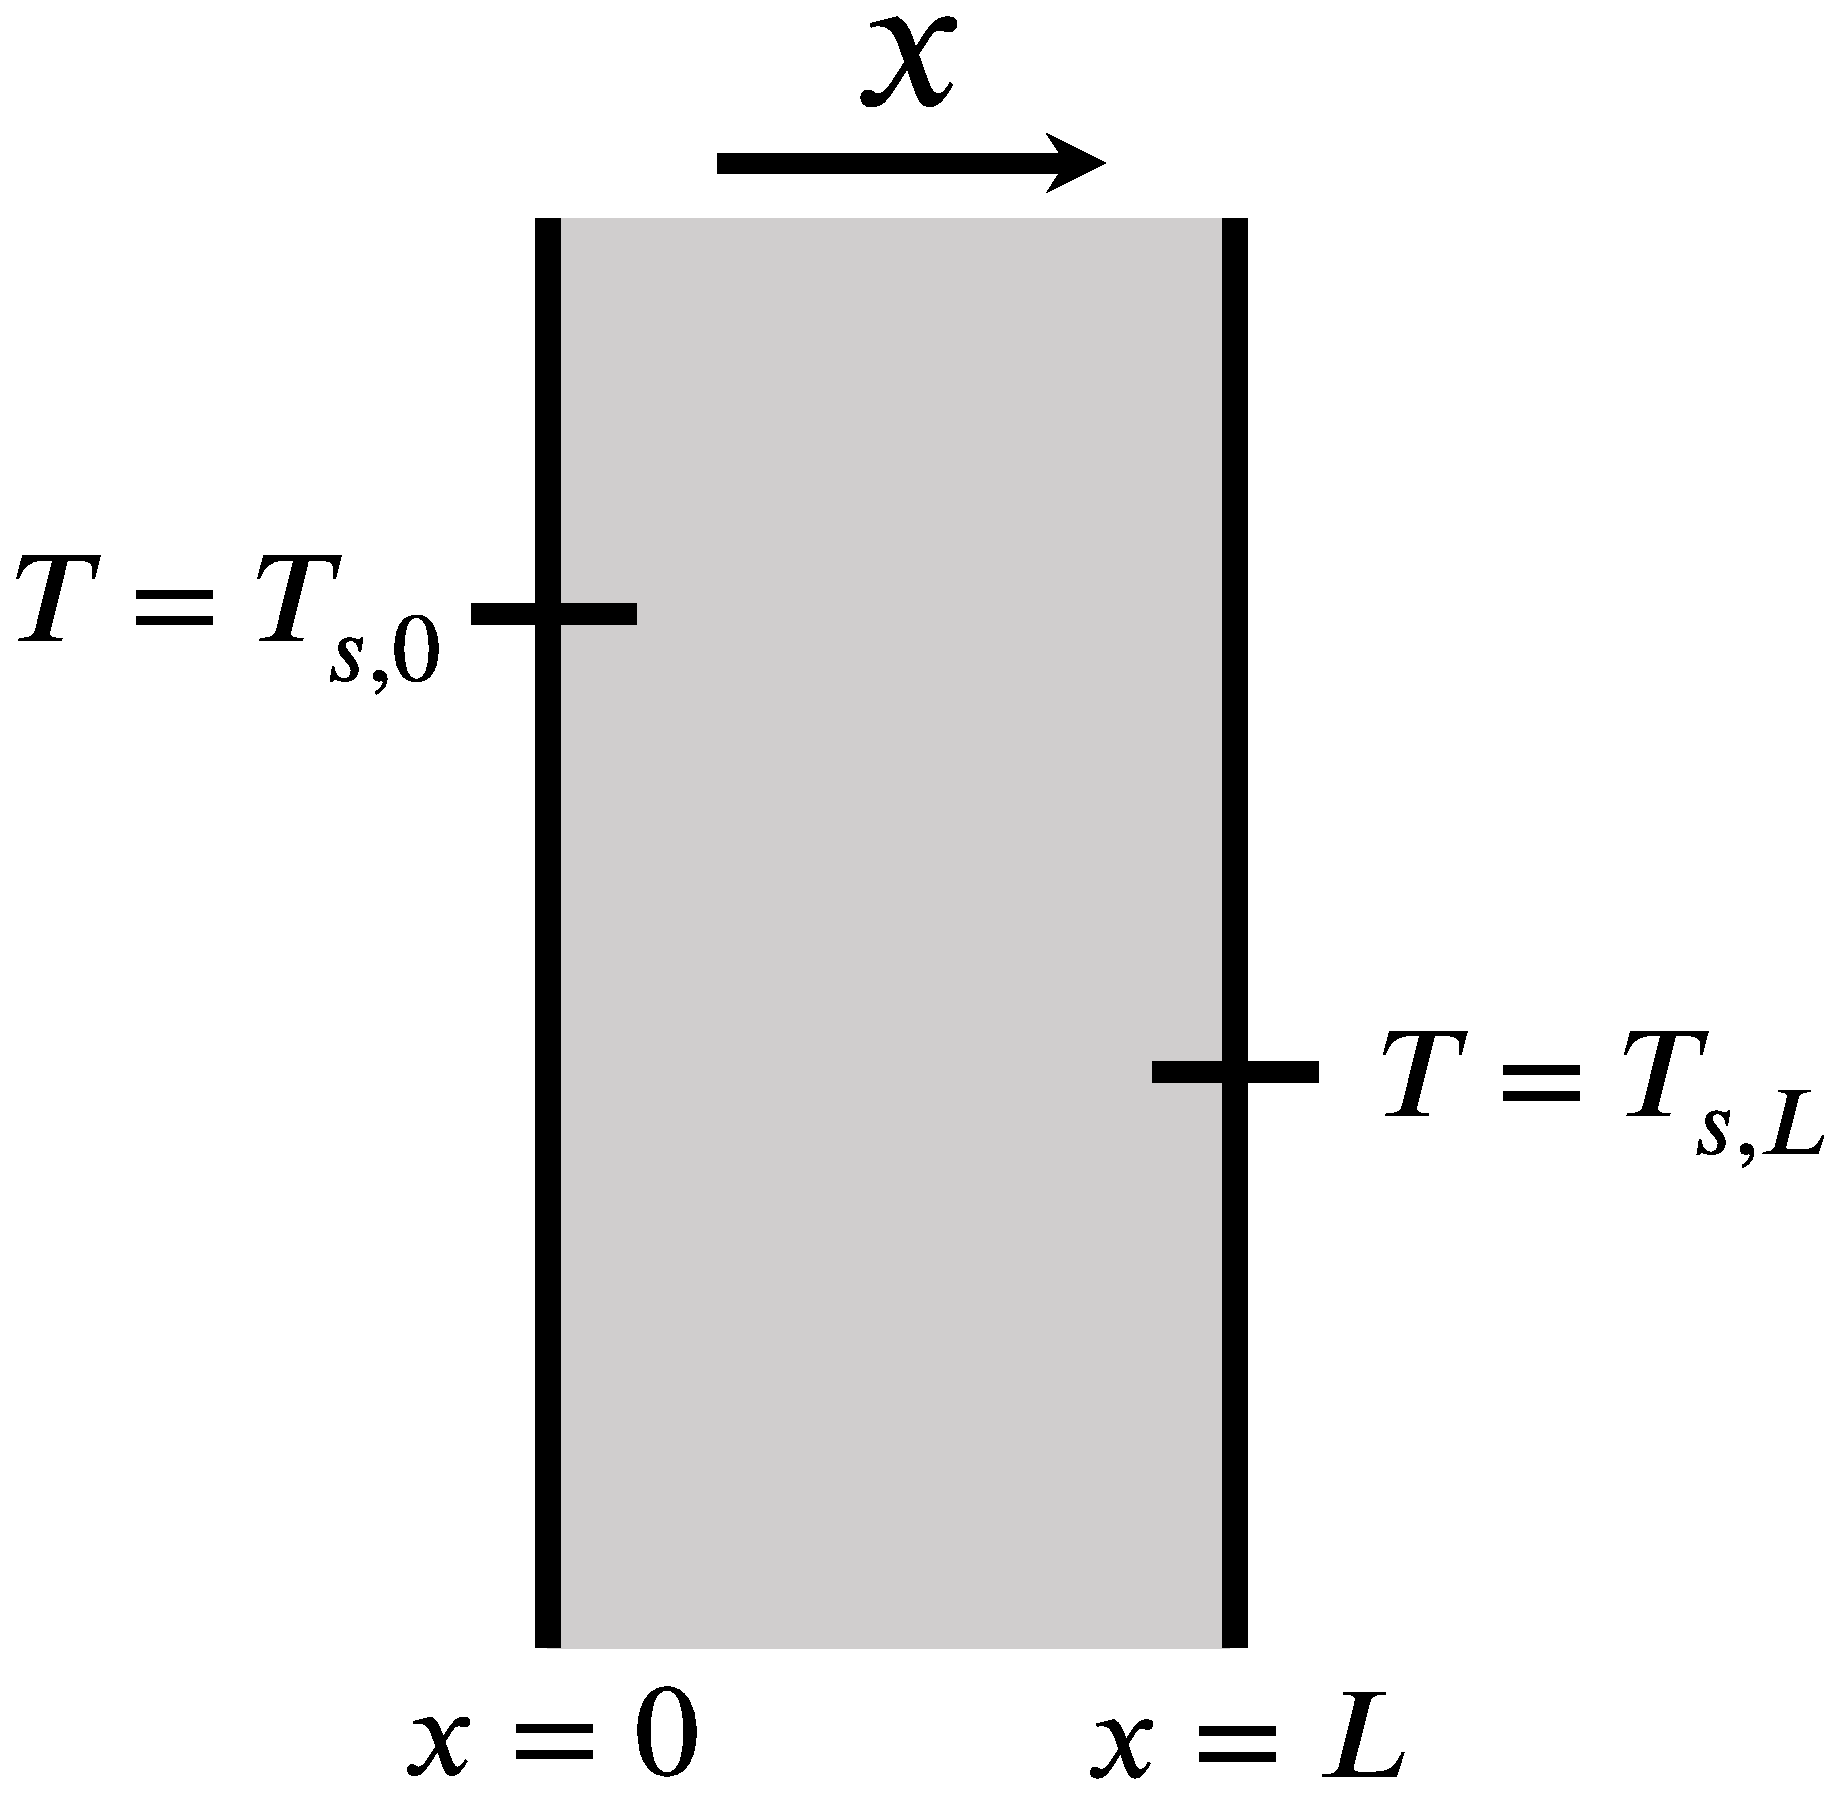
\includegraphics[width=.9\textwidth]{img/oneD_conduction_wall.eps}
\end{minipage}
\ \\
\paragraph{Solution Procedure} Start from the heat equation:
\[ 
    \rho c_{p}\bigg( \cancelto{0}{\frac{\partial T}{\partial t}} +\cancelto{0}{(\bm{v} \cdot \nabla) T} \bigg) = \cancelto{0}{\dot{S_{v}}} +k \nabla^{2} T 
\]
Rearrange,
\[ 
    \frac{\mathrm{d}^{2} T}{\mathrm{d} x^{2}}=0 \quad \Rightarrow \quad T = C_{1}x + C_{2} 
\]
Impose the Dirichlet boundary conditions for constants $C_1$ and $C_2$: 
\begin{itemize}
    \item $\displaystyle x=0, \ T = T_{s,0} \ \Rightarrow \ C_{2} = T_{s,0}$ 
    \item $\displaystyle x=L, \ T = T_{s, L} \ \Rightarrow \ C_{1}=\frac{T_{s,L}-T_{s,0}}{L}$
\end{itemize}
Therefore,
\[ 
    T(x) = \frac{T_{s,L}-T_{s,0}}{L} x + T_{s,0}
\]
which has a \textit{linear} profile, decreasing from $T_{s,0}$ to $T_{s, L}$ from $x=0$ to $x=L$. 
\begin{center}
    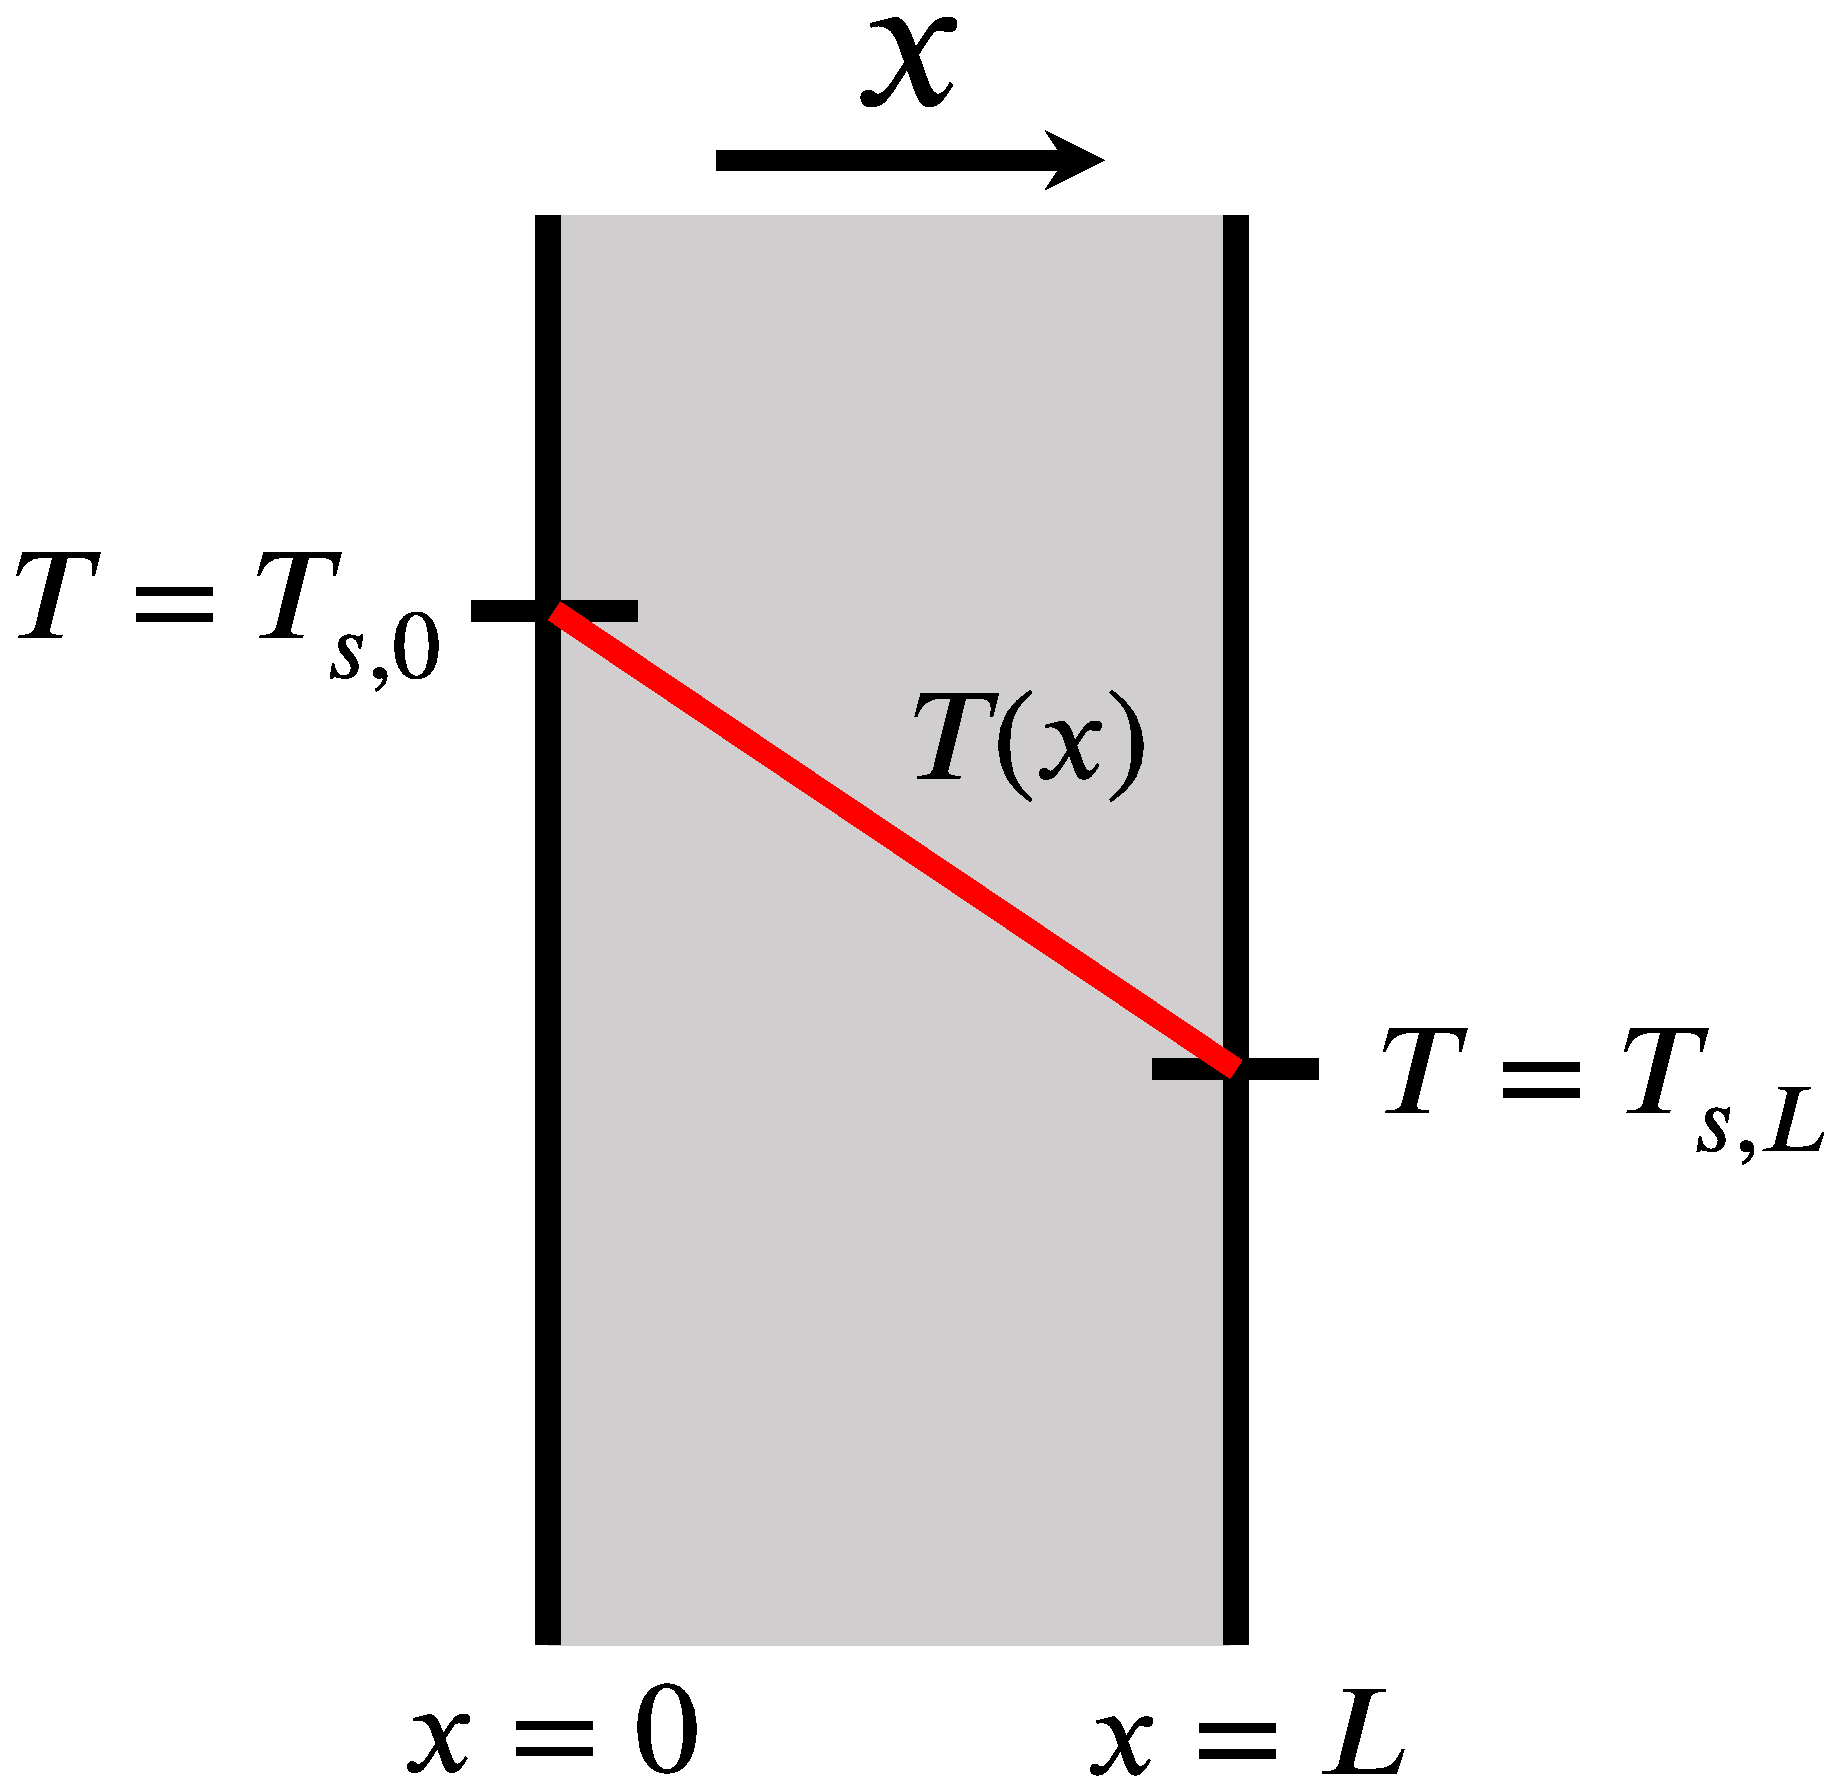
\includegraphics[width=.4\textwidth]{img/oneD_conduction_wall_solution.eps}
\end{center}

The flux, 
\[ 
    q = \frac{k}{L} \Delta T = \frac{k}{L} (T_{s,0}-T_{s,L}) 
\]
which is a \textit{constant}.
\end{tcolorbox}

%==========================================================
\subsubsection{Thermal Resistance}
The linear temperature profile from the above example allows us to use the concept of \textbf{resistance} to construct an equivalent ``\textbf{thermal circuit}''.

\paragraph{Thermal Resistance} Analogous to the electrical resistance, 
\begin{table}[H] 
\centering
\begin{tabular}{c|c}
    \toprule
    \textbf{current flow} $I${\color{gray}[$\mathrm{A}$]} & \textbf{heat flux} $\dot{Q}${\color{gray}[$\mathrm{W}$]}  \\ 
    \midrule
    $\displaystyle I = \frac{1}{R} \Delta V$  & $\displaystyle \dot{Q} =\frac{k A}{L} \Delta T $ \\ \midrule
    \begin{circuitikz} 
    \draw
        (0,0) node[label={[font=\footnotesize]above:$V_{1}$}]{} to [R, *-*, R=$R$, v=$\Delta V$] (3,0) node[label={[font=\footnotesize]above:$V_{2}$}]{};
    \end{circuitikz} & 
    \begin{circuitikz} 
    \draw
        (0,0) node[label={[font=\footnotesize]above:$T_{1}$}]{} to [R, *-*, R=$\frac{L}{kA}$, v=$\Delta T$] (3,0) node[label={[font=\footnotesize]above:$T_{2}$}]{};
    \end{circuitikz}
    \\
    \bottomrule
\end{tabular}
\end{table}
the \textbf{thermal resistance} of heat conduction, $\displaystyle R_{T,cond} = \frac{L}{kA} \ {\color{gray}\bigg[\frac{\mathrm{K}}{\mathrm{W}}\bigg]}$, impedes the process of conduction. \\
\begin{itemize}
    \item For other modes of heat transport in a \textit{plane wall}, the thermal resistances are
    \begin{table}[H]
        \centering
        \begin{tabular}{c c c}
        \toprule
        \textbf{Conduction}, $R_{T, cond}$  &   \textbf{Convection}, $R_{T, conv}$  &   \textbf{Radiation}, $R_{T, rad}$ \\ \midrule
        $\displaystyle \frac{L}{kA}$  &   $\displaystyle \frac{L}{hA}$  &   $\displaystyle \frac{L}{h_{r}A}$\\
        \bottomrule
        \end{tabular}
    \end{table}

    \item For different geometries, the thermal resistances for \textit{conduction} are
    \begin{table}[H]
        \centering
        \begin{tabular}{lc}
            \toprule
            \textbf{Geometry}   &  \textbf{Thermal Resistance, $R_{T, cond}$} \\
            \midrule
            plane wall          &  $\displaystyle \frac{L}{kA}$ \\ [1.2em]
            cylindrical wall    &  $\displaystyle \frac{\ln(r_{2}/r_{1})}{2\pi LA}$ \\[1.2em]
            spherical wall      &  $\displaystyle \frac{1}{4\pi k} (\frac{1}{r_{1}}-\frac{1}{r_{2}})$ \\
            \bottomrule
        \end{tabular}
    \end{table}
\end{itemize}

\paragraph{Contact Resistance} Conduction across the true contact area. Convection/radiation across gaps.


\subsection{Example 2: Steady-State Conduction in a Cylinder}
\begin{tcolorbox}[breakable, title = \textbf{Example: Conduction Through a Cylinder}]
\begin{minipage}{.6\textwidth}
    \paragraph{Assumptions} 
    \begin{itemize}
        \item 1-D steady-state conduction $\Rightarrow \partial / \partial t = 0$;
        \item no external heat generation $ \Rightarrow \dot{S}_{v} = 0$;
        \item no convection is considered $\Rightarrow (\bm{v} \cdot \nabla) T = 0$;
        \item constant $k$.
\end{itemize}

\paragraph{Aim} Solve for $T(r)$ in wall.
\end{minipage}
\hfill
\begin{minipage}{.4\textwidth}
    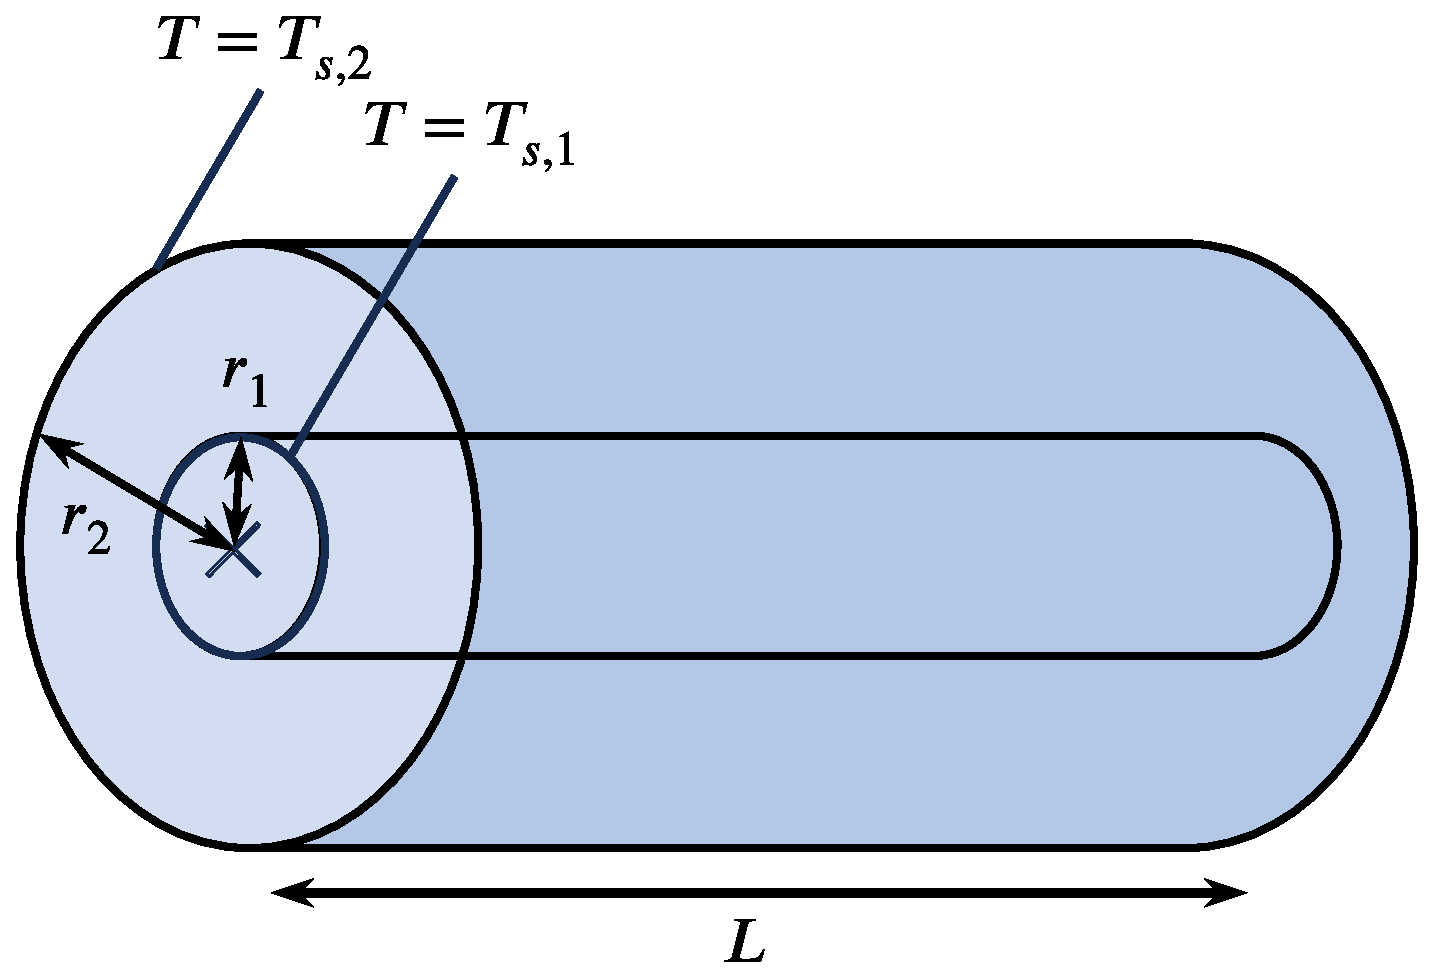
\includegraphics[width=\textwidth]{img/oneD_conduction_cylinder.eps}
\end{minipage}
\vspace{.2cm}
\hrule
\vspace{.2cm}
\textbf{Solution Procedure} Start from the heat equation:
\[ 
    \rho c_{p}\bigg(\cancelto{0}{\frac{\partial T}{\partial t}} +\cancelto{0}{(\bm{v} \cdot \nabla) T} \bigg) = \cancelto{0}{\dot{S_{v}}} + k\nabla^{2} T 
\]
In cylindrical coordinates:
\[ 
    \nabla^{2} T = \frac{1}{r}\frac{\partial}{\partial r} \bigg(r\frac{\partial T}{\partial r}\bigg)+ \frac{1}{r^{2}} \cancelto{0}{\frac{\partial^{2}T}{\partial \theta^{2}}}+\cancelto{0}{\frac{\partial^{2}T}{\partial z^{2}} }
\]
Therefore:
\[ 
    \nabla^{2} T = 0 \ \Rightarrow \ T=C_{1} \ln(r)+C_{2} 
\]
Impose the Dirichlet boundary conditions for constants $C_1$ and $C_2$: 
\begin{itemize}
    \item $\displaystyle r=r_{1}, T=T_{s,1} \ \Rightarrow \ C_{1}=\frac{T_{s,1}-T_{s,2}}{\ln(r_{1}/r_{2})}$
    \item $\displaystyle r=r_{2}, T=T_{s,2} \ \Rightarrow \ C_{2}=T_{s,2}-\frac{T_{s,1}-T_{s,2}}{\ln(r_{1}/r_{2})}\ln(r_{2})$
\end{itemize}
Therefore,
\[ 
    T(r) = \frac{T_{s,1}-T_{s,2}}{\ln(r_{1}/r_{2})} \ln \bigg(\frac{r}{r_{2}}\bigg) + T_{s,2} 
\]

\end{tcolorbox}

%==========================================================
\subsection{Example 3: Wall Exposed to Convection}
\begin{tcolorbox}[breakable, title = \textbf{Example: Wall Exposed to Convection}]
\begin{minipage}{.6\textwidth}
    \paragraph{Assumptions}
    \begin{itemize}
        \item 1-D steady-state conduction $\Rightarrow \partial / \partial t = 0$;
        \item no external heat generation $ \Rightarrow \dot{S}_{v} = 0$;
        \item exposed to fluid convection $T_{\infty}$ at $x = L$;
        \item constant $k$.
    \end{itemize}
    \paragraph{Aim} Solve for $T(x)$ in wall.
\end{minipage}
\begin{minipage}{.35\textwidth}
    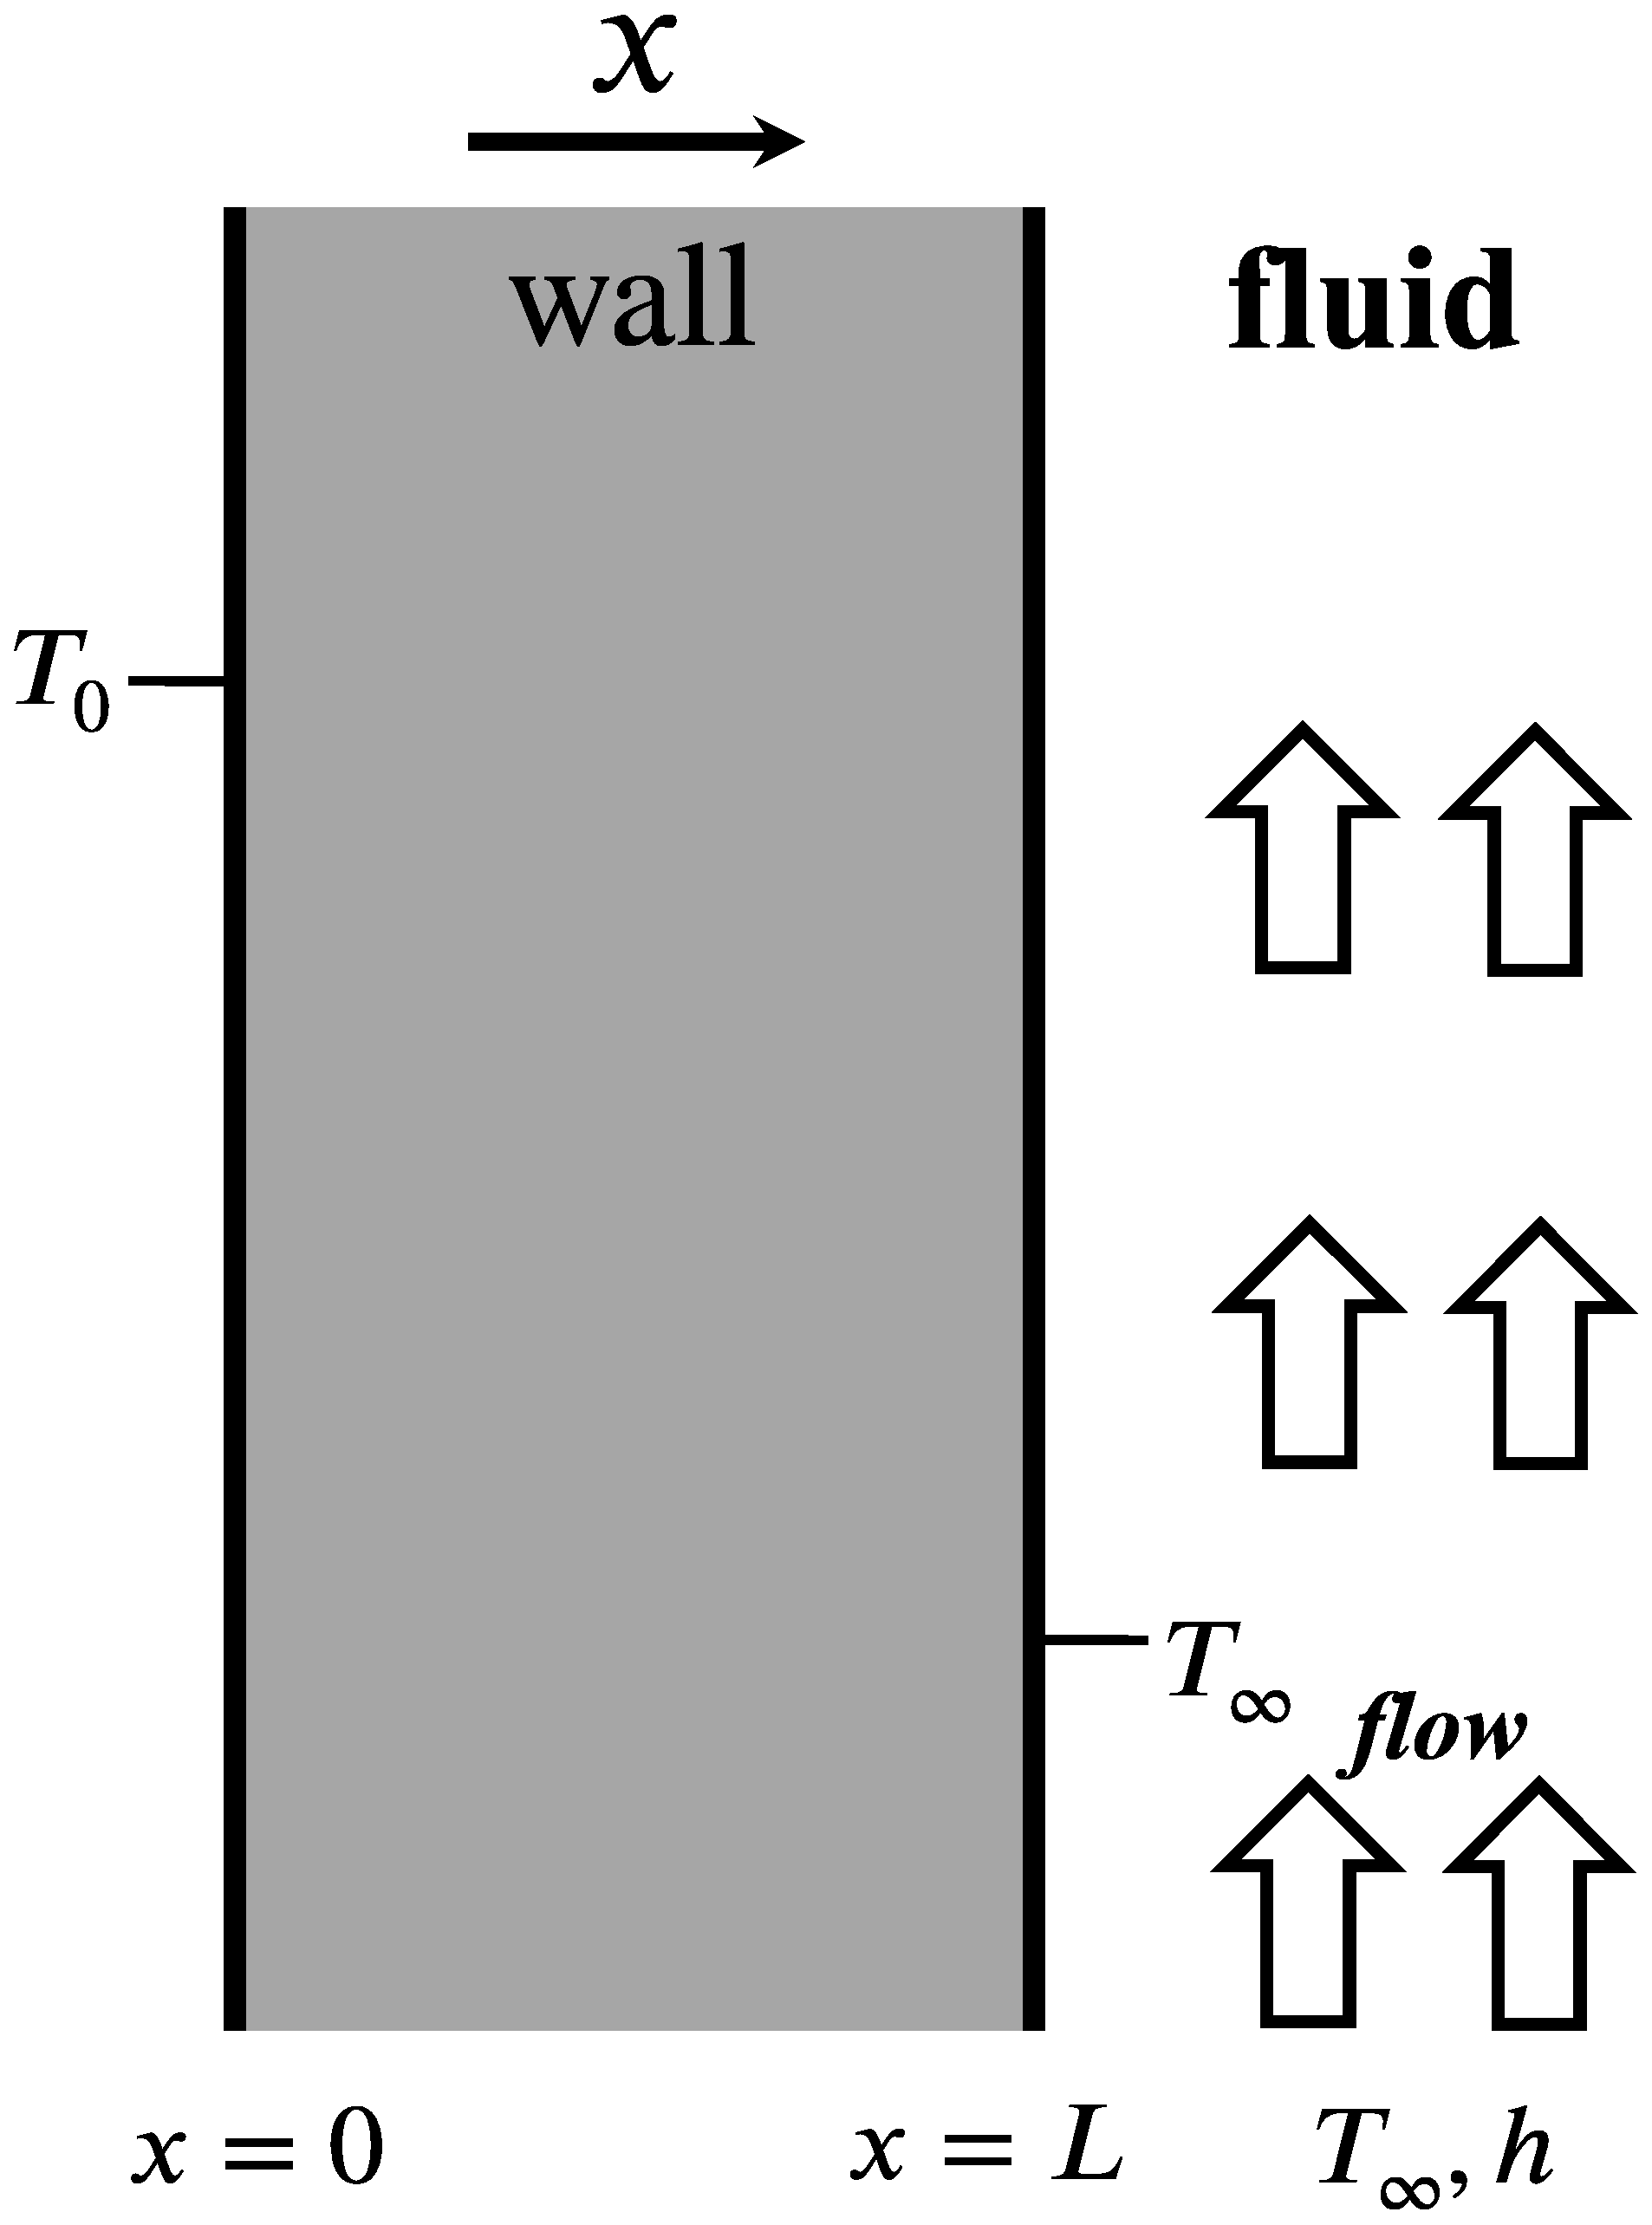
\includegraphics[width=.9\textwidth]{img/conduction_convection.eps}
\end{minipage}

\textbf{Solution Procedure} \quad
Start from the heat equation:
\[ 
    \rho c_{p}\bigg(\cancelto{0}{\frac{\partial T}{\partial t}} +\cancelto{0}{(\bm{v} \cdot \nabla) T}\bigg) = \cancelto{0}{\dot{S_{v}}}  +k \nabla^{2} T 
\]
Rearrange,
\[ 
    \frac{\mathrm{d}^{2} T}{\mathrm{d} x^{2}} \ \Rightarrow \ T = C_{1}x + C_{2} 
\]
Impose the boundary conditions for constants $C_1$ and $C_2$:
\begin{itemize}
    \item Dirichlet condition: $\displaystyle x=0, \ T = T_{0} \quad \Rightarrow \quad C_{2}=0$
    \item Newton's Law of Cooling: $\displaystyle x=L, \ -k\frac{\mathrm{d}T}{\mathrm{d}t}=h(T_{0}-T_{\infty}) \ \Rightarrow \ C_{1}=-\frac{h(T_{0}-T_{\infty})}{k+hL}$
\end{itemize}
Therefore,
\[ 
    T(x) = -\frac{h(T_{0}-T_{\infty})}{k+hL}x + T_0
\]
\paragraph{How does the temperature profile within the wall look like?} The gradient of $T(x)$ is $\displaystyle -\frac{h(T_{0}-T_{\infty})}{k+hL}$. Since $T_0 - T_\infty$ is constant, what determines the temperature distribution within the wall is the term $\displaystyle \frac{h}{k+hL}$ (ignore the minus symbol) $\Rightarrow$ need to discuss the following cases
\begin{itemize}
    \item $h>>k$, \textit{i.e.}, convection is greater than conduction;
    \item $h \approx k$, \textit{i.e.}, convection is about the same as conduction;
    \item $h<<k$, \textit{i.e.}, conduction is grater than convection.
\end{itemize}
We thus introduce the Biot number, $Bi$, that represents the ratio of convection to conduction.
\end{tcolorbox}

\subsubsection{The Biot Number}
The Biot number, $Bi$, is a dimensionless number, that represents the relative magnitude of \textit{surface convection} to \textit{conduction within a solid}.
\[ 
    Bi = \frac{\frac{L}{kA}}{\frac{1}{hA}} = \frac{hL}{k} = \frac{\text{temperature drop in wall}}{\text{temperature drop across surface}}   \quad \mathrm{{\color{gray} \bigg[ \frac{ W/(m^2\cdot K) \cdot m}{W/(m\cdot K)}\bigg]}}
\]
\begin{itemize}
    \item if $Bi<<1$: convection is more dominant $\Rightarrow$ assume \textit{uniform} temperature within solid;
    \item if $Bi>>1$: cannot assume uniform temperature within solid.
\end{itemize}
Therefore, the temperature profile within the solid from the above example
\begin{figure}[H]
    \centering
    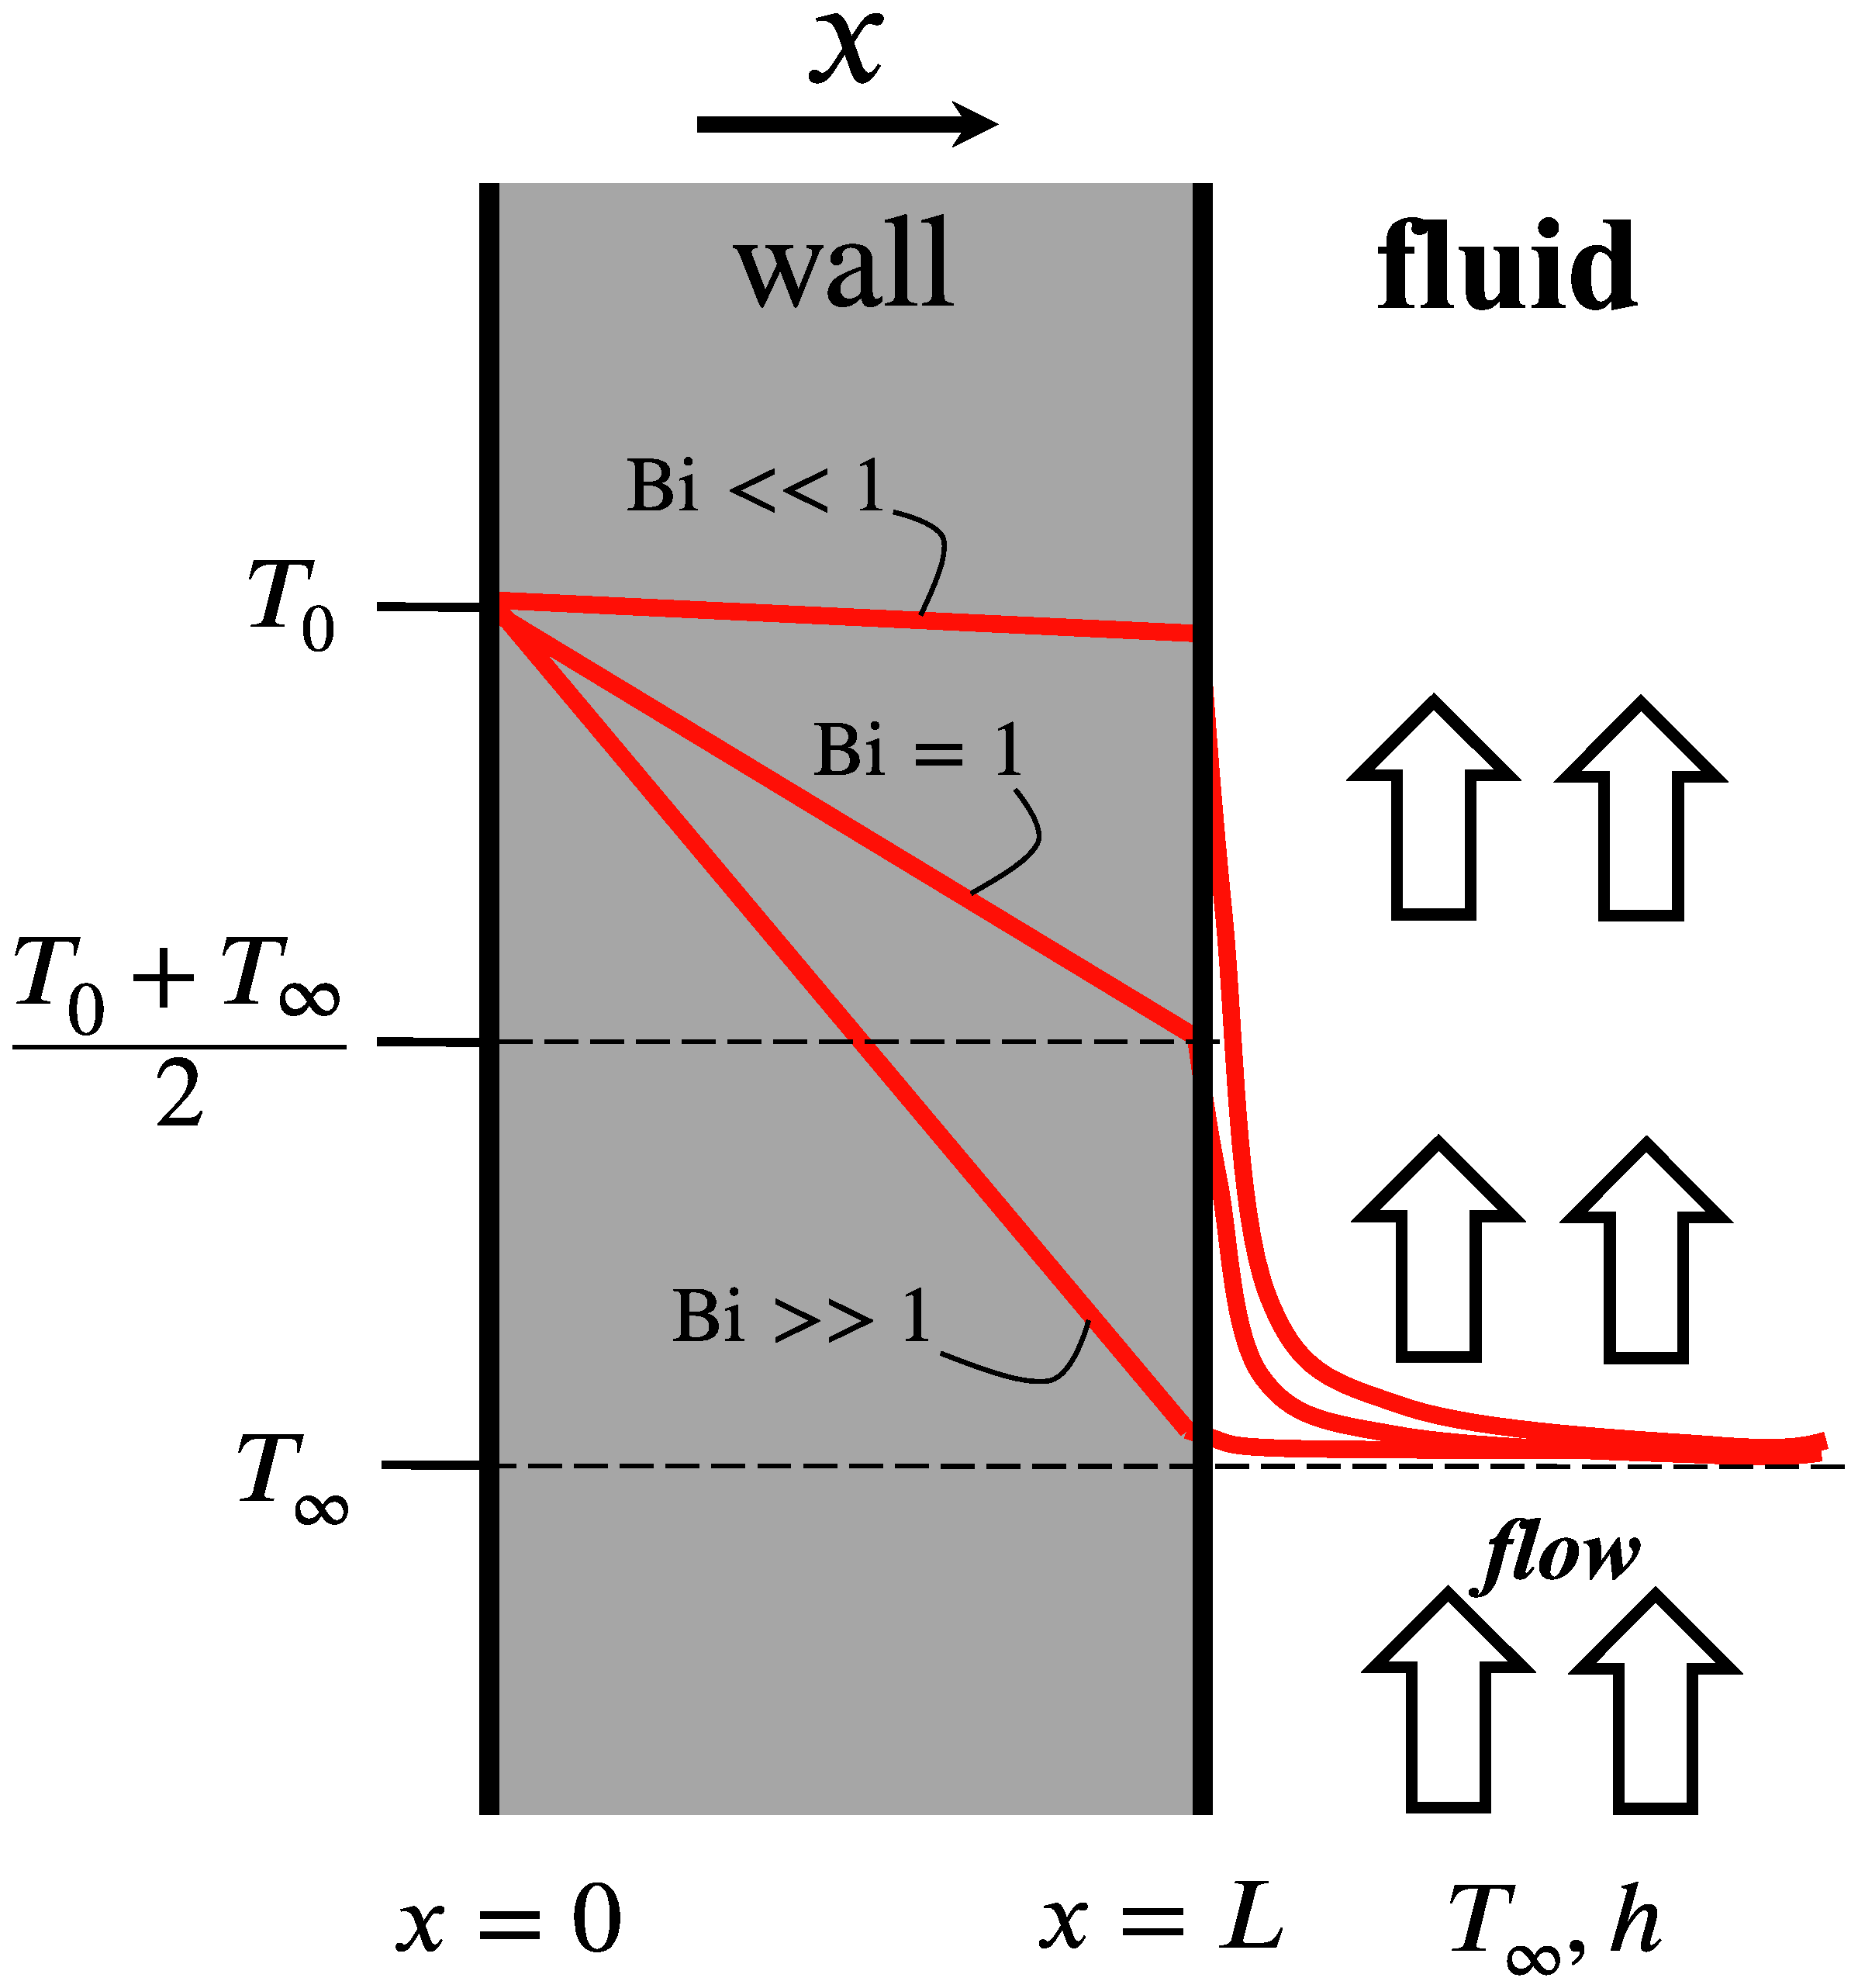
\includegraphics[width=.4\textwidth]{img/conduction_convection_solution.eps}
\end{figure}


%==========================================================
\subsection{Example 4: Internal Heat Generation}

\begin{tcolorbox}[breakable, title = \textbf{Example: Internal Heat Generation}]
\begin{minipage}{.6\textwidth}
    \paragraph{Assumptions} 
    \begin{itemize}
        \item 1-D steady-state conduction  $\Rightarrow \partial / \partial t = 0$;
        \item heat generated with the rate, $\dot{S}_{v}$;
        \item no convection is considered $\Rightarrow (\bm{v} \cdot \nabla) T = 0$;
        \item exposed to fluid convection at $x=L$.
    \end{itemize}
    \paragraph{Aim} Solve for $T(x)$ in wall.
\end{minipage}
\begin{minipage}{.4\textwidth}
    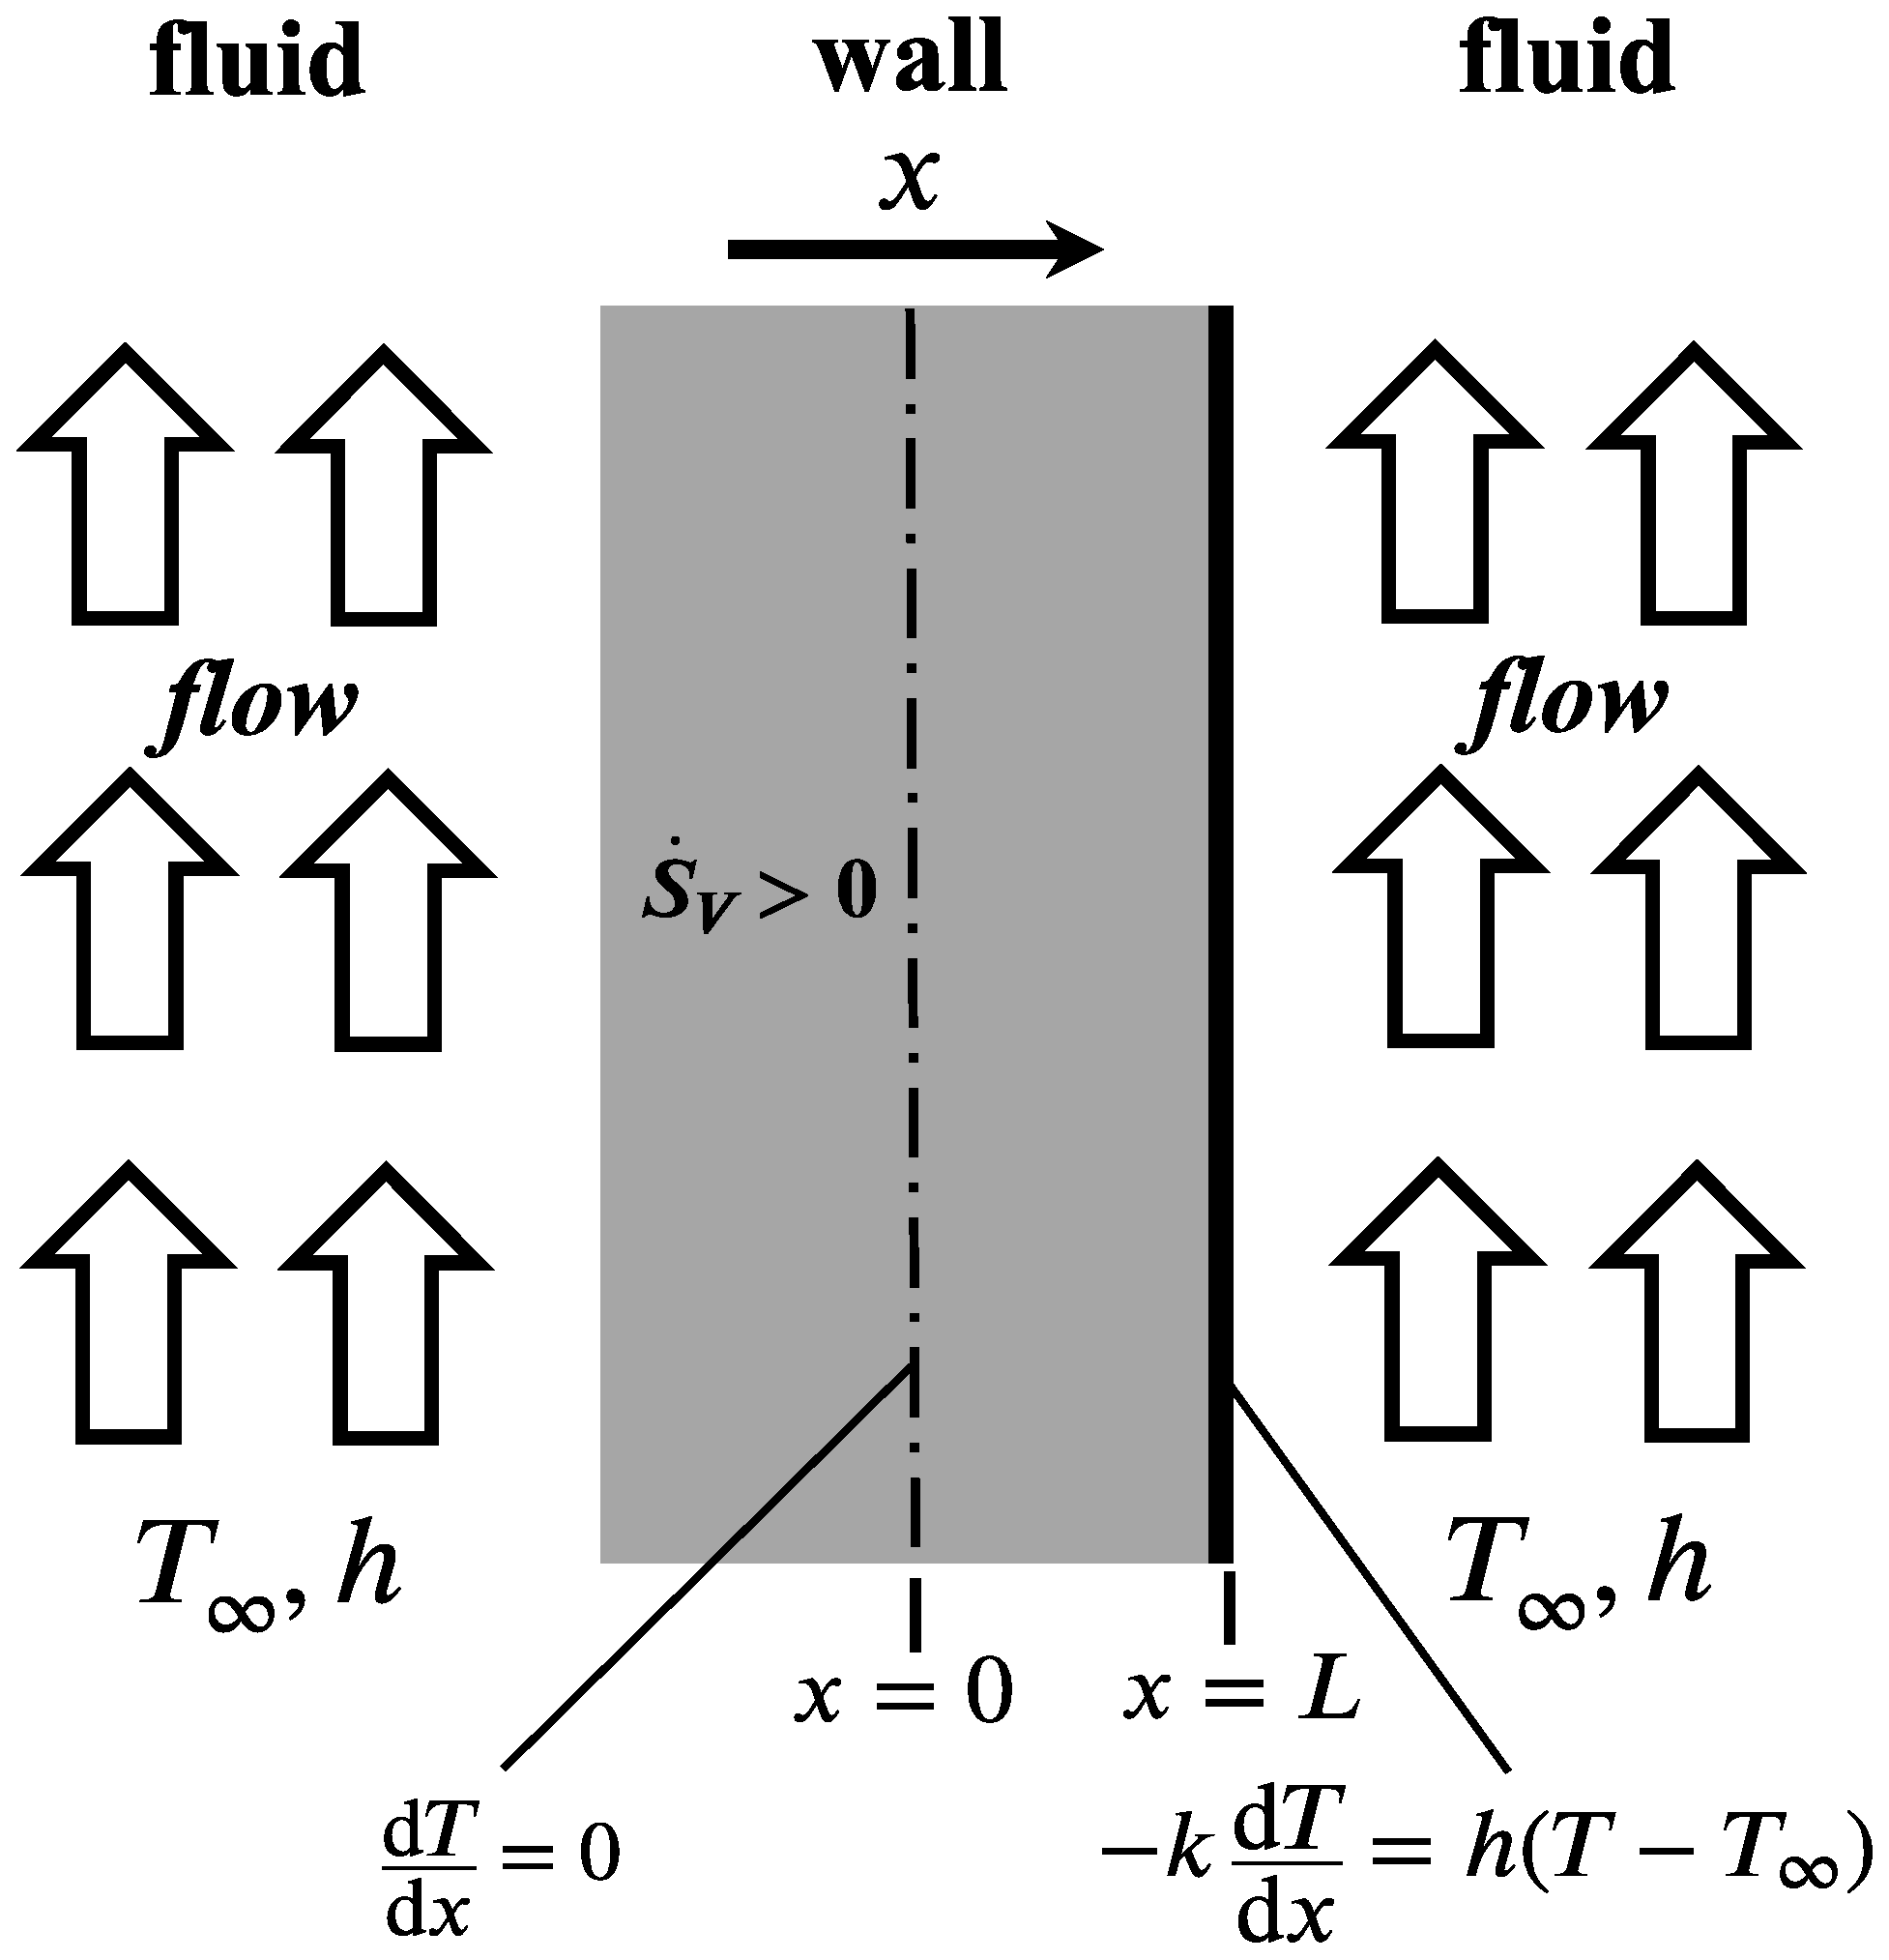
\includegraphics[width=\textwidth]{img/internal_heat_gen.eps}
\end{minipage}

\textbf{Solution Procedure} \quad 
\emph{N.B.} We take advantage of the geometry symmetry, thus setting the coordinate origin $x=0$ in the middle and only considering half of the geometry. \\
Start from the heat equation:
\[ 
    \rho c_{p} \bigg( \cancelto{0}{\frac{\partial T}{\partial t}} +\cancelto{0}{(\bm{v} \cdot \nabla) T} \bigg) = \dot{S_{v}}  +k \nabla^{2} T 
\]
Rearrange,
\[ 
    \frac{\mathrm{d}^{2} T}{\mathrm{d}x^{2}} + \dot{S_{v}}=0 \quad \Rightarrow \quad T = -\frac{\dot{S_{v}}}{2k}x^{2}+C_{1}x + C_{2}
\]
Impose the boundary conditions for constants $C_1$ and $C_2$:
\begin{itemize}
    \item Neumann condition: $\displaystyle x=0, \frac{\mathrm{d}T}{\mathrm{d}t}=0 \ \Rightarrow \  C_{1}=0$
    \item Newton's Law of Cooling: $\displaystyle x=L, \ -k\frac{\mathrm{d}T}{\mathrm{d}t}=h(T-T_{\infty}) \ \Rightarrow \ C_{2}=\frac{\dot{S_{v}}L}{h}+\frac{\dot{S_{v}}L^{2}}{2k}+T_{\infty}$ 
\end{itemize}
Therefore,
\[
    T(x) = \frac{\dot{S_{v}}L^{2}}{2k} \bigg( 1-\frac{x^{2}}{L^{2}} \bigg) + \frac{\dot{S_{v}}L}{h} + T_{\infty} 
\]
\begin{figure}[H]
    \centering
    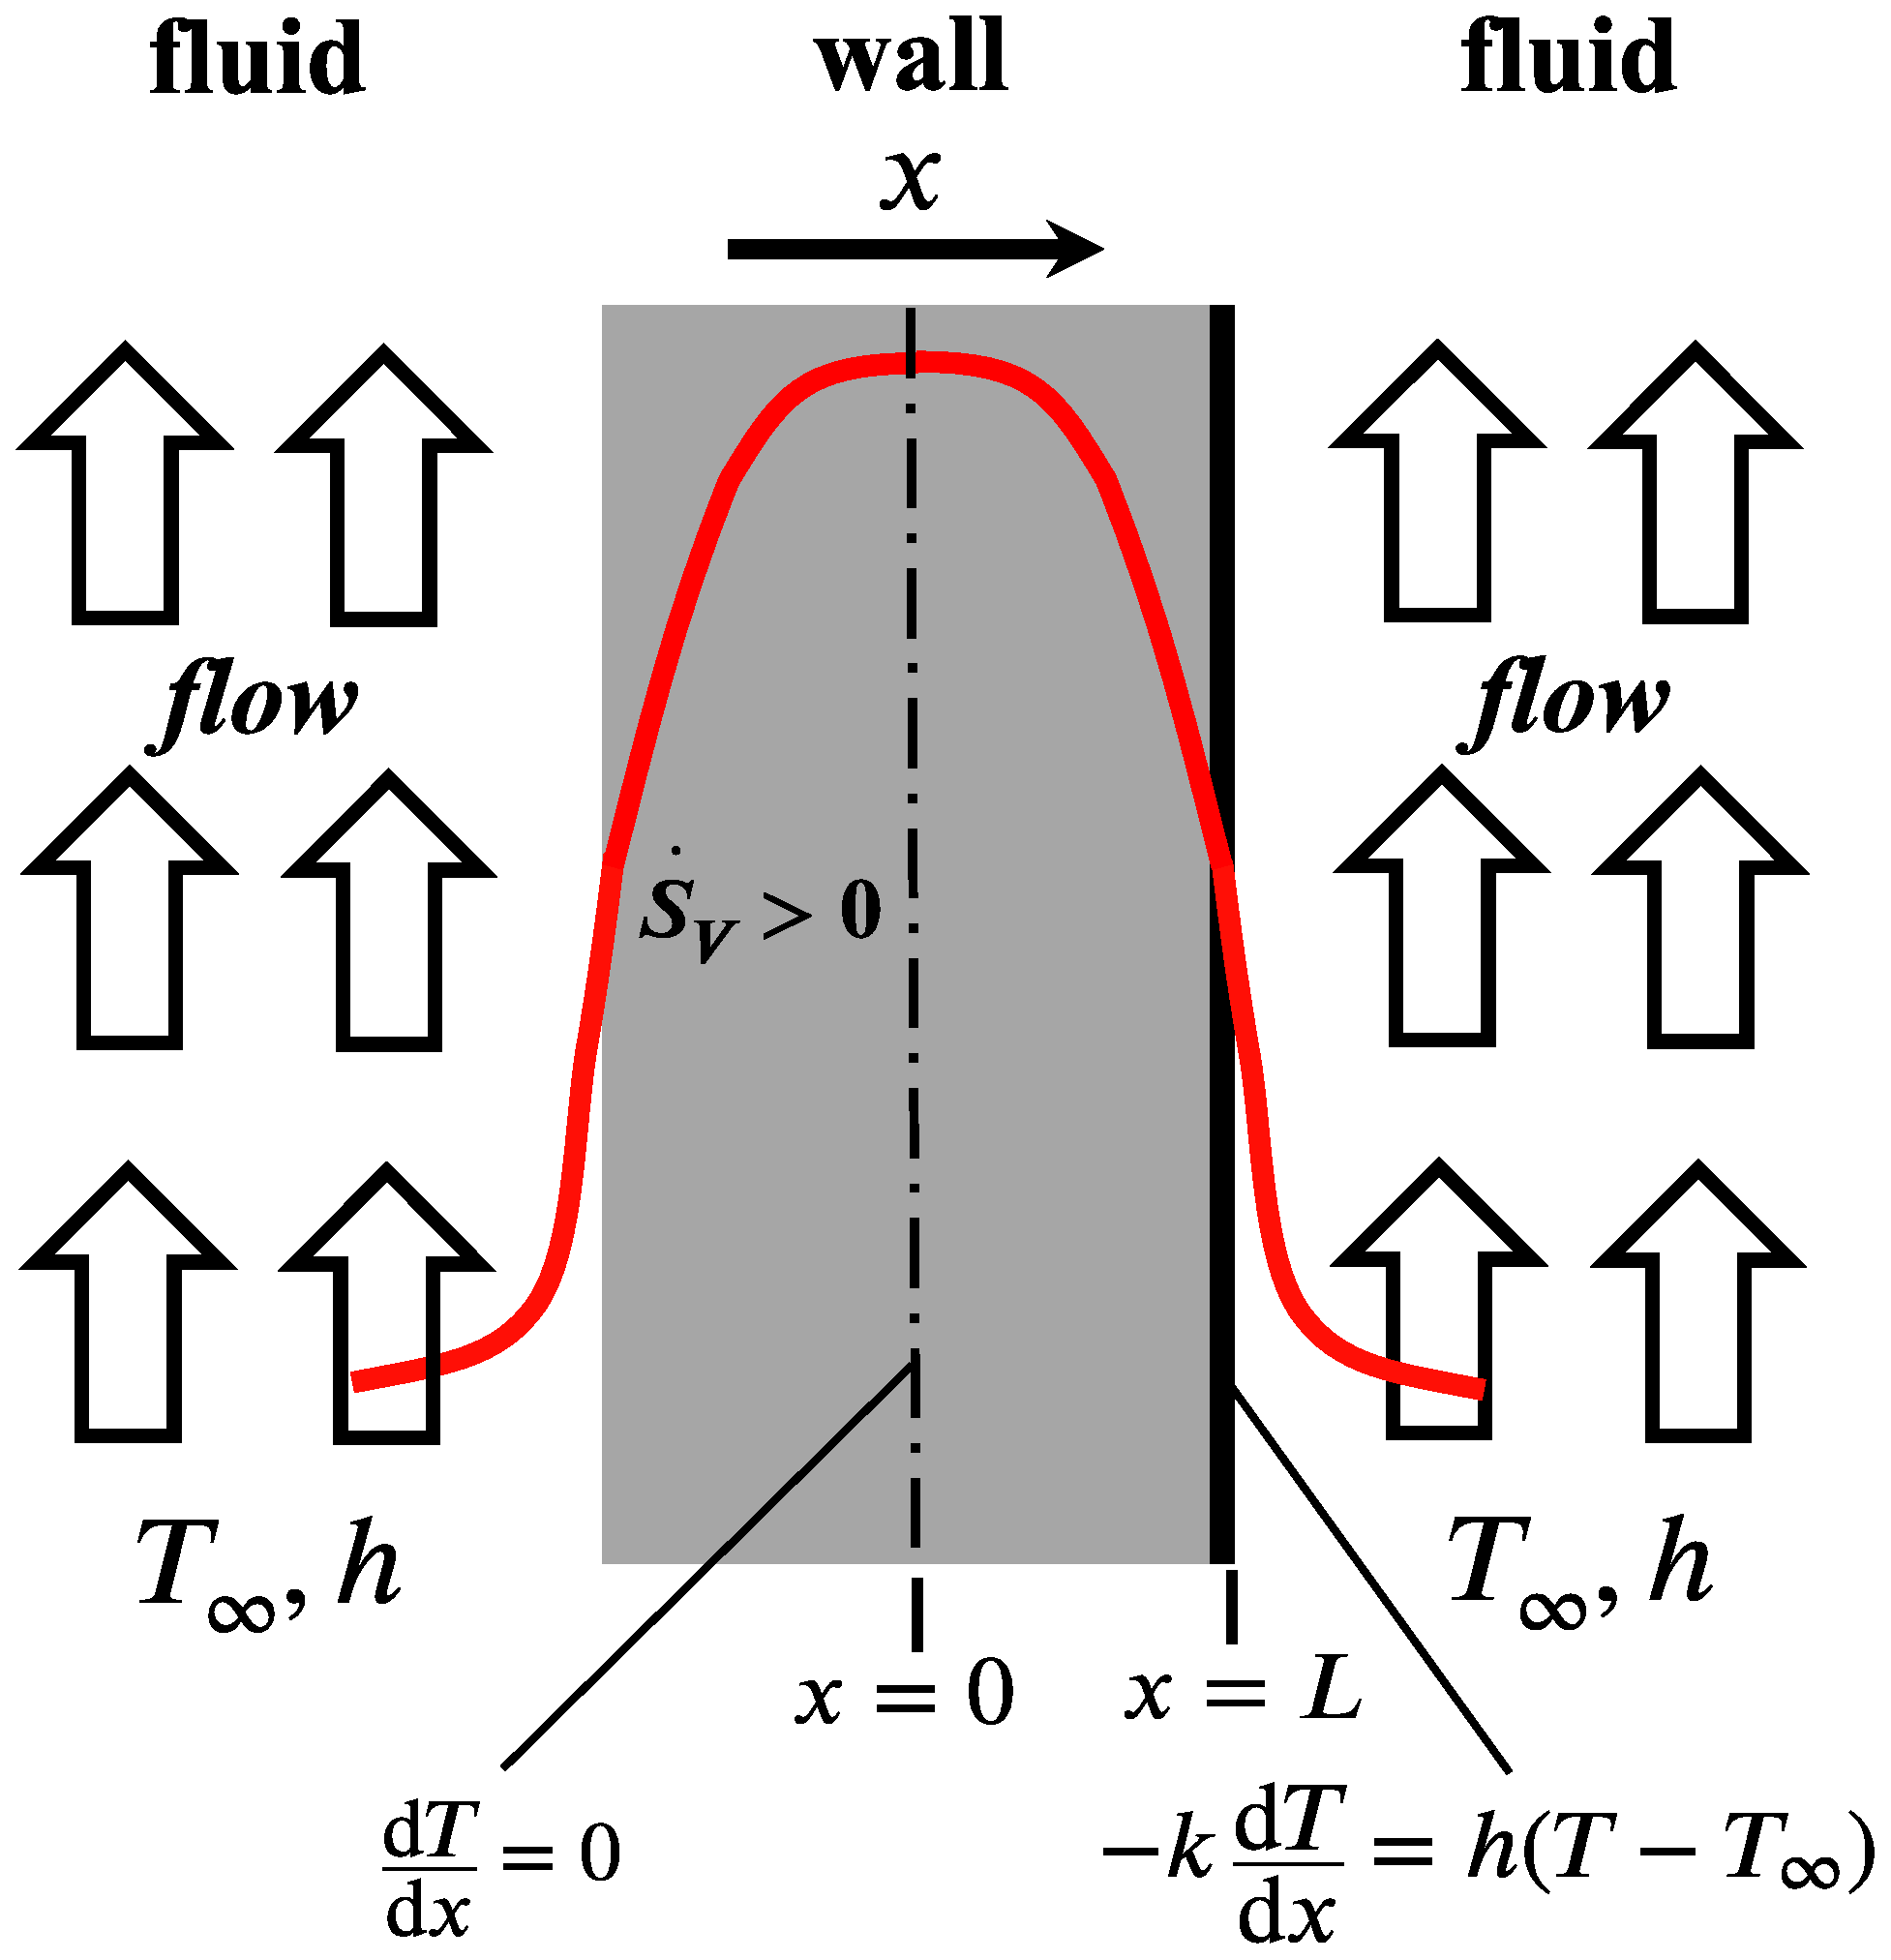
\includegraphics[width=.4\textwidth]{img/internal_heat_gen_solution.eps}
\end{figure}
\paragraph{Symmetry of the solution along the centreline} As we only solved the solution from $x=0$ to $x=L$ (right half of the geometry), the full temperature profile can be obtained by mapping the solution along the centreline.
\end{tcolorbox}



% \begin{tcolorbox}[breakable, title = Example]%Need graphs
% Given $\displaystyle Bi = \frac{hL}{k}$,
% \begin{align*} 
% \begin{split} 
%     T 
%     &= T_{0}-\frac{(T_{0}-T_{\infty})}{(\frac{k}{hL}+1)}\frac{x}{L}\\
%     &= T_{0}-\frac{Bi (T_{0}-T_{\infty})}{Bi+1}\frac{x}{L}
% \end{split} 
% \end{align*}
% \begin{itemize}
%     \item if $Bi<<1$, $T \approx T_{0}-Bi(T_{0}-T_{\infty})\frac{x}{L}$
%     \item if $Bi>>1$, $T \approx T_{0}-(T_{0}-T_{\infty})\frac{x}{L}$
% \end{itemize}
% Given $x=L, \ T = T_{L} \ \to \ -k\frac{dT}{dx}=h(T_{L}-T_{\infty})$, and intuitively: $\displaystyle \frac{dT}{dx} \sim \frac{T_{L}-T_{0}}{L}$
% \[ 
%     \therefore \ -k \frac{T_{L}-T_{0}}{L} \sim h(T_{L}-T_{\infty}) \ \to \ \boxed{\frac{T_{0}-T_{L}}{T_{L}-T_{\infty}} \sim \frac{hL}{k} = Bi} 
% \]
% \[
%     Bi = \frac{\text{temperature drop in wall}}{\text{temperature drop across surface}} 
% \]
% \end{tcolorbox}

% %%Similarity Variable
% Define dimensionless variables:
% \begin{itemize}
%     \item $T^{*} = \frac{T}{\hat{T}}$, where $\hat{T}$ is the characteristic temperature scale;
%     \item $t^{*} = \frac{t}{\hat{t}}$, where $\hat{t}$ is the characteristic time scale;
%     \item $x^{*} = \frac{x}{\hat{x}}$, where $\hat{x}$ is the characteristic length scale;
% \end{itemize}

% \[
%     \frac{\partial T}{\partial t} = \alpha \frac{\partial^{2}T}{\partial x^{2}}
% \]
% Using chain rule:
% \[
%     \frac{\hat{T}}{\hat{t}} \frac{\partial T^{*}}{\partial t^{*}} = \frac{\alpha \hat{T}}{\hat{x}^{2}} \frac{\partial^{2}T^{*}}{\partial x^{*2}}
% \]
% Since equation must be satisfied at every point in space:
% \[
%     \frac{1}{\hat{t}} \frac{\partial T^{*}}{\partial t^{*}} = \frac{\alpha}{\hat{x}^{2}} \frac{\partial^{2}T^{*}}{\partial x^{*2}}
% \]
% This indicates that 
% \[
%     \frac{1}{\hat{t}} \mathtt{\sim}  \frac{\alpha}{\hat{x}^{2}} \longrightarrow \hat{x} = \sqrt{\alpha \hat{t}}
% \]
% \[
%     \eta = \frac{x}{2\sqrt{\alpha t}}
% \]
% \begin{itemize}
%     \item If $\eta <<1$, front has already passed;
%     \item If $\eta >>1$, front not yet arrived.
% \end{itemize}

% \subsection{Internal Heat Generation - 1D conduction with heat generation}
% \begin{tcolorbox}[breakable, title = \textbf{Example}]
%     \paragraph{Assumptions}
%     \begin{itemize}
%         \item 1-D steady-state conduction through wall;
%         \item the wall exposed to the fluid convection at $x=L$.
%     \end{itemize}
%     \paragraph{Aim} Find the temperature distribution, $T(x)$, in wall.
%     \paragraph{Boundary condition}
%     \begin{itemize}
%         \item Newton's law of cooling at $x=L$:
%             $\displaystyle -k\frac{\mathrm{d}T}{\mathrm{d}x} = h(T-T_{\infty}) \quad \text{at} \quad x=L$
%         \item Symmetry condition at $x = 0$:
%             $\displaystyle \frac{\mathrm{d}T}{\mathrm{d}x} = 0 \quad \text{at} \quad x=0$
%     \end{itemize}

% Start from xx
% \[
%     \rho c_{p}\bigg\{ \frac{\partial T}{\partial t} + (\bm{v}\cdot \nabla)T\bigg\} = k\nabla^{2}T + \dot{S}_{v}
% \]
% Applying the assumptions above, the heat equation is reduced to 
% \[
%     \frac{\mathrm{d}^{2}T}{\mathrm{d}x^{2}} = -\frac{\dot{S}_{v}}{k}
% \]
% Thus, the general solution can be obtained by integrating the second-order ODE twice:
% \[
%     T = -\frac{\dot{S}_{v}}{2k}x^{2} + C_{1}x +C_{2}
% \]
% where $C_{1}$, $C_{2}$ are two constants to be determined. \\
% Substituting the boundary conditions above into the general solution, two constants $C_{1}$, $C_{2}$ can be found. 
% \[
%     C_{1} = 0\quad \text{and} \quad C_{2} = \frac{\dot{S}_{v}L}{h}+\frac{\dot{S}_{v}L^{2}}{2k}+T_{\infty}
% \]
% Therefore, the temperature distribution, $T(x)$, in this 1D solid wall with internal heat generation is
% \[
%     T(x) = \frac{\dot{S}_{v}L^{2}}{2k}\bigg(1-\frac{x^{2}}{L^{2}}\bigg) + \frac{\dot{S}_{v}L}{h} + T_{\infty}
% \]
% \paragraph{Interpretation} At $x=L$, $\displaystyle T(L) = \frac{\dot{S}_{v}L}{h} + T_{\infty}$. Rearrange the expression $\displaystyle \Rightarrow T_{L}-T_{\infty} = \frac{\dot{S}_{v}L}{h}$. By control volume analysis, at steady state, the total rate of heat production in the control volume must be balanced by the total rate of heat flow out of the control volume by convection. 
% \end{tcolorbox}


\newpage
\section{Transient Heat Conduction}
\subsection{Lumped Capacitance Method}
\begin{figure}[H]
    \centering
    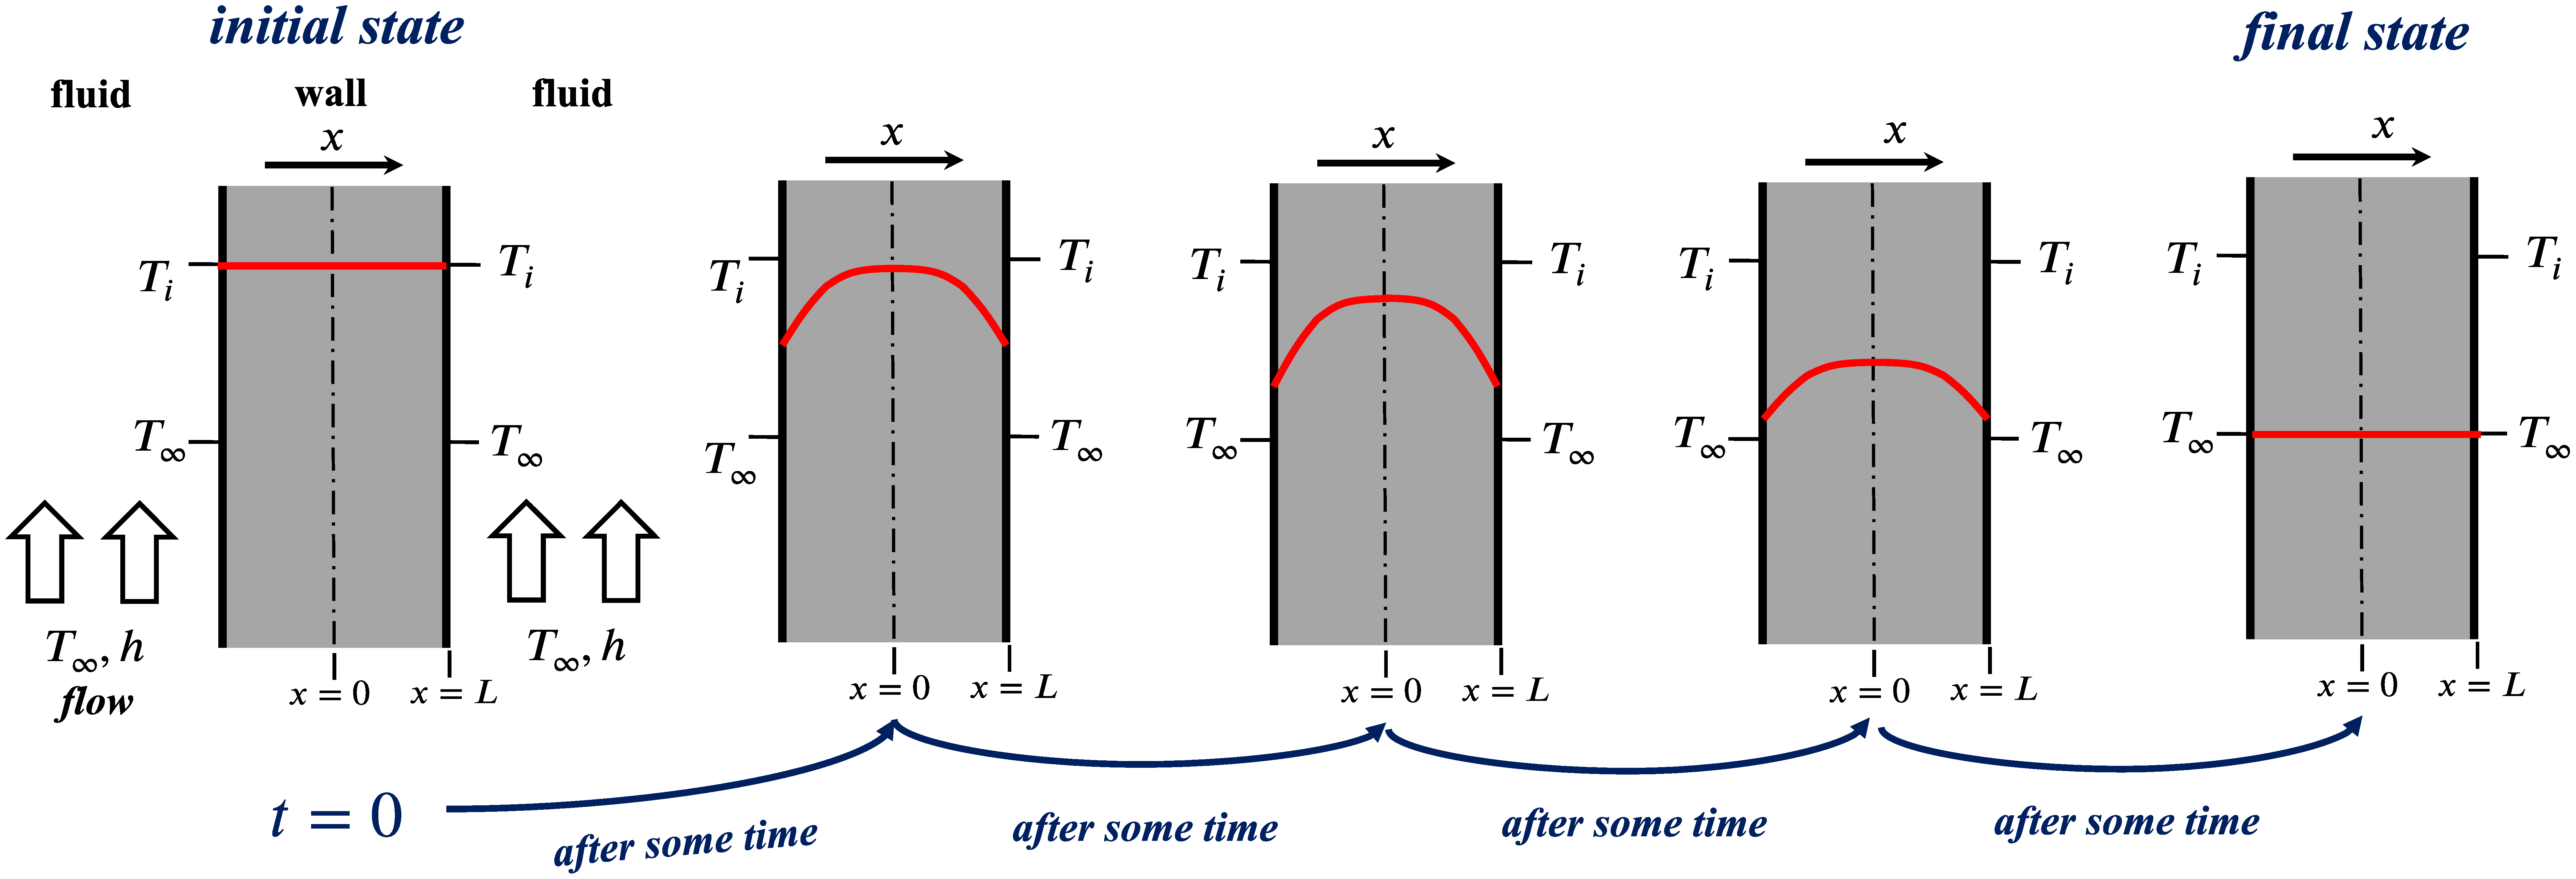
\includegraphics[width=\textwidth]{img/temporal_propagation.eps}
\end{figure}

\paragraph{Problem Formulation} Consider a planar wall at an initial uniform temperature $T_i$ -
\begin{itemize}
    \item At $t = 0$, the wall is exposed to fluid at temperature $T_\infty$;
    \item Time-dependent changes in wall temperature from $T_i$ to $T_\infty$ (figure).
\end{itemize}
No convection and heat generation were considered. 
% The governing equation is
% \begin{equation}
%     \label{eqn:transient_heat_eqn}
%     \frac{\partial T}{\partial t} = \alpha \frac{\partial^2 T}{\partial x^2}
% \end{equation}
% where $\displaystyle \alpha = \frac{k}{\rho c_p}$ is the thermal diffusivity (m\textsuperscript{2}/s). 
Given the initial and boundary conditions $(x, t)$:
\begin{itemize}
    \item {\color{gray}[IC]} At $t=0^-$ (\textit{immediately} before the initial convection exposure), $T = T_i$, for all $x \geq 0$
    \item {\color{gray}[BC]} At $x=0$, $T = T_s$, for all $t \geq 0^+$ (after the convection exposure)
    \item {\color{gray}[BC]} At $x \to \infty$, $T \to T_i$, for all $t \geq 0^+$
\end{itemize}

\paragraph{Aim} Determine the temperature profile $T(x, t)$.

\paragraph{Solution Procedure}
If $Bi << 1$: temperature is nearly \textit{uniform} within the solid at each point in time,
\begin{itemize}
    \item Conduction is very fast within the solid;
    \item Convection is very slow from the contact surface.
\end{itemize}
Therefore, we could simplify the problem $T(x, t) \to T(t)$.\\

Start from the differential form of the heat equation,
\[
    \frac{\partial}{\partial t} \int\limits_{CV} \rho c_{p} T \mathrm{d}V = \cancelto{0,\text{no source}}{\int\limits_{CV} \dot{S_{v}} \mathrm{d}V} - \oint\limits_{CS} (\bm{q} \cdot \bm{\hat{n}}) \mathrm{d}A - \cancelto{0,\text{no advection}}{\oint\limits_{CS} \rho c_{p} T (\bm{v} \cdot \bm{n}) \mathrm{d}A}
\]
As $\rho$, $c_p$ and $T$ are uniform within CV, only $T$ changes with time ($\partial \to \mathrm{d}$):
\[
    \rho c_p V \frac{\mathrm{d} T}{\mathrm{d} t} = -q_h A \quad \Rightarrow \quad 
    \rho c_p V\frac{\mathrm{d} T}{\mathrm{d} t} = -\underbrace{h(T-T_\infty)}_{q_h} A
\]
The above equation states the balance of the \textit{rate of change of the thermal energy} and \textit{the convective heat transfer from surface}. \\

It can be further re-arranged to a first-order ODE:
\[
    \frac{\mathrm{d}T}{\mathrm{d} t} = -\frac{hA}{\rho c_pV}(T-T_\infty)
\]
Define two parameters $\Theta = T-T_\infty$, $\displaystyle \tau = \frac{\rho c_pV}{hA}$,
\[
    \frac{\mathrm{d}\Theta}{\mathrm{d} t} = -\frac{1}{\tau}\Theta \quad \xrightarrow[]{\text{solve the ODE}} \quad \Theta = C_1 e^{-t/\tau}
\]
where the constant $C_1$ is subjected to the initial condition $\Rightarrow C_1 = T_i-T_\infty$. The general solution is
\[
    \Theta = (T_i-T_\infty) e^{-t/\tau} \quad \xrightarrow[\Theta = T-T_\infty]{\text{expand}} \quad \boxed{T = (T_i-T_\infty) e^{-t/\tau} + T_{\infty}}
\]
\begin{figure}[H]
    \centering
    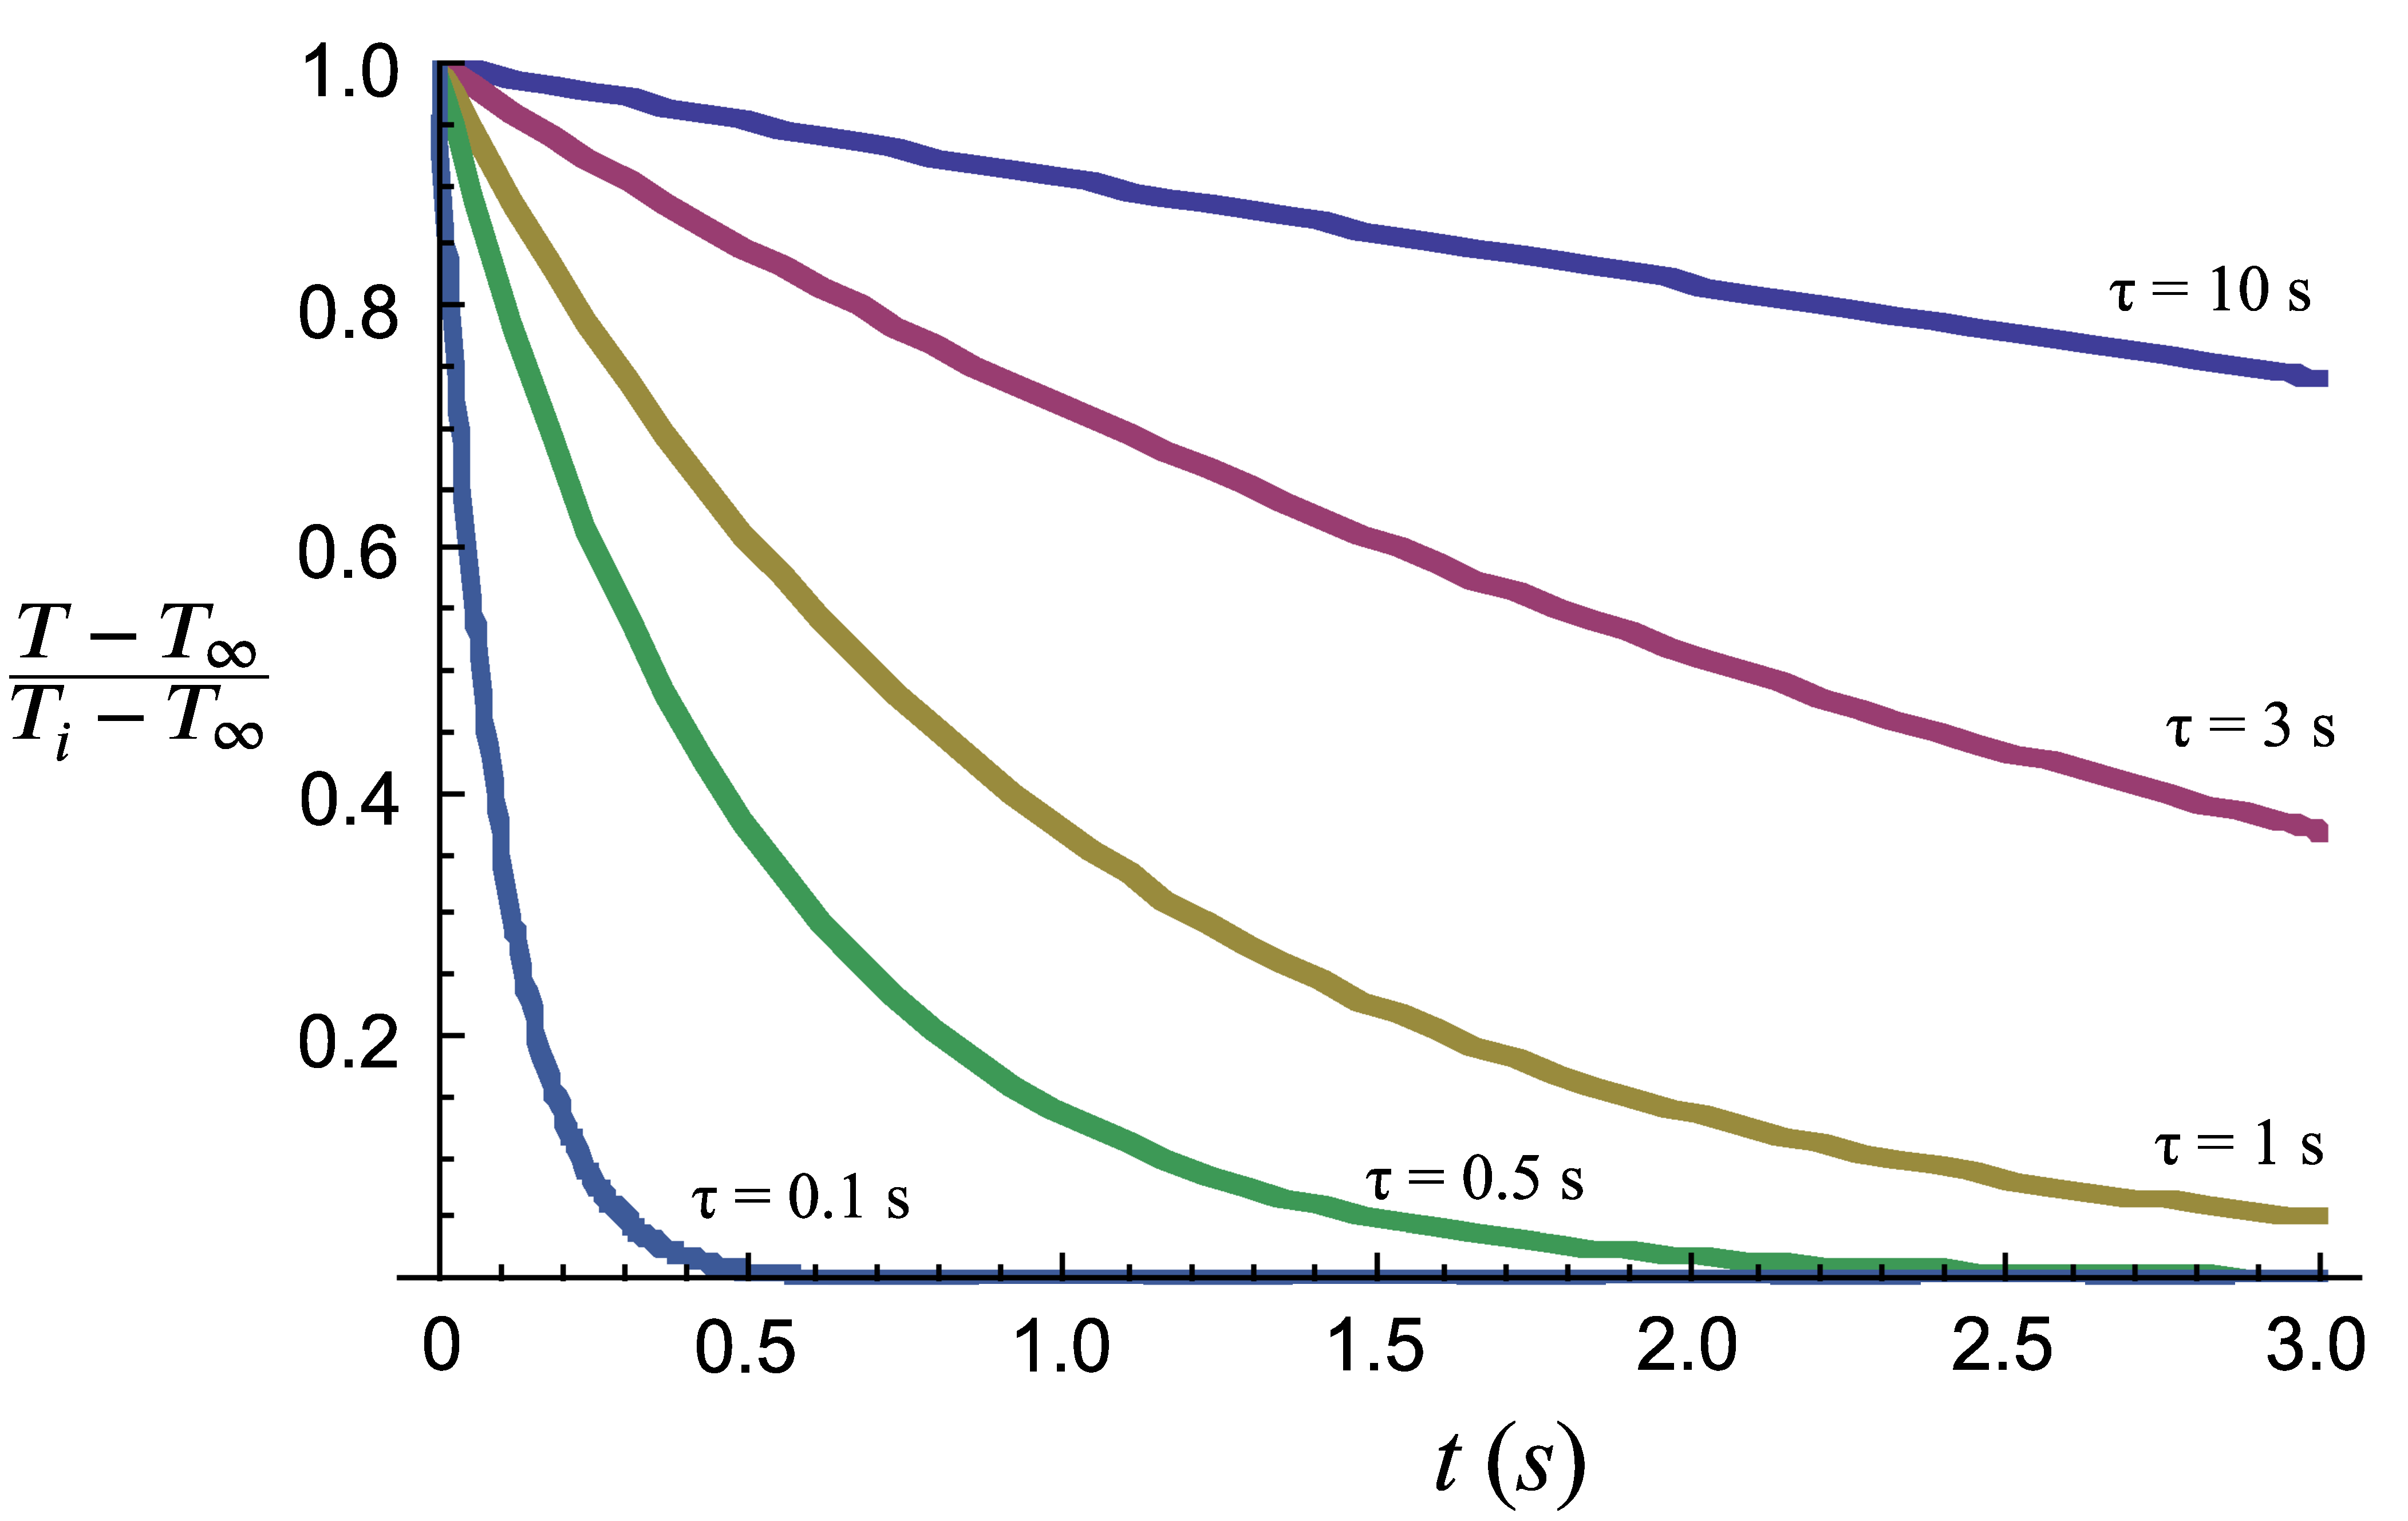
\includegraphics[width=.7\textwidth]{img/lumped_capacitance_solution.eps}
\end{figure}
where $\displaystyle \tau = \frac{\rho c_pV}{hA} = \underbrace{\frac{1}{hA}}_{R_t} \ \underbrace{\rho c_p V}_{C_t}$ can be interpreted as the product of thermal resistance ($R_t$) and the heat capacity of the wall ($C_t$).
\begin{figure}[H]
    \centering
    \begin{circuitikz} 
    \draw
        (0, 0) -- (1, 0)  node{} to [R, *-*, R=$R_t$] (1,-2) node{}
        (1, 0) -- (2.5, 0) node{}  to [C, *-*, C=$C_t$] (2.5, -2)
        (2.5, -2) -- (0, -2) to[closing switch] (0,0);
    \end{circuitikz}
\end{figure}



\subsection{Transient Conduction through Semi-Infinite Solid}
Start from the differential form of the heat equation,
\[
    \rho c_{p} \bigg( \frac{\partial T}{\partial t} +\cancelto{0}{(\bm{v} \cdot \nabla) T} \bigg) = \cancelto{0}{\dot{S_{v}}}  +k \nabla^{2} T \quad \Rightarrow \quad \frac{\partial T}{\partial t} = \alpha \frac{\partial^2 T}{\partial x^2}
\]
% %%Similarity Variable
Define dimensionless variables:
\begin{itemize}
    \item $T^{*} = \frac{T}{\hat{T}}$, where $\hat{T}$ is the characteristic temperature scale;
    \item $t^{*} = \frac{t}{\hat{t}}$, where $\hat{t}$ is the characteristic time scale;
    \item $x^{*} = \frac{x}{\hat{x}}$, where $\hat{x}$ is the characteristic length scale.
\end{itemize}
Using chain rule:
\[
    \frac{\partial T}{\partial t} = \alpha \frac{\partial^2 T}{\partial x^2}
    \quad \Rightarrow \quad
    \frac{\hat{T}}{\hat{t}} \frac{\partial T^{*}}{\partial t^{*}} = \frac{\alpha \hat{T}}{\hat{x}^{2}} \frac{\partial^{2}T^{*}}{\partial x^{*2}} \quad \xrightarrow[]{\text{divide by} \ \hat{T}} \quad \frac{1}{\hat{t}} \frac{\partial T^{*}}{\partial t^{*}} = \frac{\alpha}{\hat{x}^{2}} \frac{\partial^{2}T^{*}}{\partial x^{*2}}
\]
Since $\displaystyle \frac{\partial T^{*}}{\partial t^{*}} \sim \mathcal{O}(1)$ and $\displaystyle \frac{\partial^2 T^{*}}{\partial x^{*2}} \sim \mathcal{O}(1)$\footnote{Derivatives must be order 1.}, the remaining term must also have similarity,
\[
    \frac{1}{t^{*}} \sim \, \frac{\alpha}{x^{*2}}
    \quad \Rightarrow \quad x^{*} \sim \, \sqrt{\alpha t^{*}}
\]
\paragraph{Given the temperature profile at time $t_1$, what does the temperature profile look like at some later time $t_2$?}




Motivated by the concept of ``self-similarity'', define a similarity variable, $\eta$
\[
    \eta = \frac{x}{2\sqrt{\alpha t}}
\]
This would allow us to perform change of variable,
\[
    \frac{\partial T}{\partial t} = \alpha \frac{\partial^2 T}{\partial x^2} \quad \Leftrightarrow \quad \boxed{-2\eta \frac{\mathrm{d}T}{\mathrm{d}\eta} = \frac{\mathrm{d}^{2}T}{\mathrm{d}\eta^{2}}}
\]
\begin{tcolorbox}[title = Derivation]
The partial differentials of $\eta$ with respect to $t$ and $x$ are
\[
    \frac{\partial \eta}{\partial t} 
    = -\frac{x\alpha}{4(\alpha t)^{\frac{3}{2}}} 
    = -\frac{1}{4} \frac{x}{\sqrt{\alpha t}}\frac{\alpha}{\alpha t}
    = -\frac{\eta}{2t}
    \quad \text{and} \quad
    \frac{\partial \eta}{\partial x} = \frac{1}{2\sqrt{\alpha t}}
\]

By chain rule, the first term in heat equation can be expressed as
    \[
        \frac{\partial T}{\partial t} = \frac{\mathrm{d}T}{\mathrm{d}\eta} \frac{\partial \eta}{\partial t} = \underbrace{-\frac{\eta}{2t} \frac{\mathrm{d}T}{\mathrm{d}\eta}}_{\text{new L.H.S.}}
    \]
the second term in heat equation can be expressed as
\[
    \frac{\partial^2 T}{\partial x^2} = \frac{\mathrm{d}^2 T}{\mathrm{d} \eta^2} \bigg( \frac{\partial \eta}{\partial x} \bigg)^2 = \underbrace{\frac{1}{4 \alpha t} \frac{\mathrm{d}^2 T}{\mathrm{d} \eta^2}}_{\text{new R.H.S.}}
\]
Equate the new L.H.S. to the new R.H.S., and rearrange, the new ODE is
\[
    -2\eta \frac{\mathrm{d}T}{\mathrm{d}\eta} = \frac{\mathrm{d}^{2}T}{\mathrm{d}\eta^{2}}
\]
\end{tcolorbox}

\[
    -2\eta \frac{\mathrm{d}T}{\mathrm{d}\eta} = \frac{\mathrm{d}^{2}T}{\mathrm{d}\eta^{2}} \ \Rightarrow \ -2 \eta \xi = \frac{\mathrm{d}\xi}{\mathrm{d}\eta} \Rightarrow \ -\int 2\eta \mathrm{d}\eta = \int \frac{1}{\xi} \mathrm{d}\xi
\]
This gives us
\[
    -\eta^2 = \ln\xi + C_1 \quad \Rightarrow \quad \xi = C_2 e^{-\eta^2}
\]
Therefore, by definition $\xi = \mathrm{d}T/\mathrm{d}\eta$:
\[
    T = C_2 \int_{0}^{\eta} e^{-s^2} \mathrm{d}s + C_3
\]
where $s$ here within the integral is a dummy variable.\\

Impose the boundary conditions:
\begin{itemize}
    \item at $\eta = 0$, $T = T_s$, $\Rightarrow C_3 = T_s$
    \item as $\eta \to \infty$, $T \to T_i$, $\Rightarrow C_2 = \frac{2(T_i - T_s)}{\sqrt{\pi}}$
\end{itemize}
Therefore, 
\[
    T =  \frac{2(T_i - T_s)}{\sqrt{\pi}} \int_{0}^{\eta} e^{-s^2} \mathrm{d}s + T_s
\]
define the \textbf{error function} $\mathrm{erf}$ as
\[
    \mathrm{erf}(z) = \frac{2}{\sqrt{\pi}} \int_{0}^{z} e^{-s^2} \mathrm{d}s
\]
and substitute
\[
    T = (T_i - T_s) \ \mathrm{erf}(\eta) + T_s
\]
Alternatively, define the \textit{Co-error function}, $\mathrm{erfc}$ as 
\[
    \mathrm{erfc}(z) = 1 - \mathrm{erf}(z)
\]
The solution becomes 
\[
    T = (T_s - T_i) \ \mathrm{erfc}(\eta) + T_i \quad \Rightarrow \quad \boxed{T = (T_s - T_i) \ \mathrm{erfc}\bigg(\frac{x}{2\sqrt{\alpha t}}\bigg) + T_i}
\]

\begin{figure}[H]
    \centering
    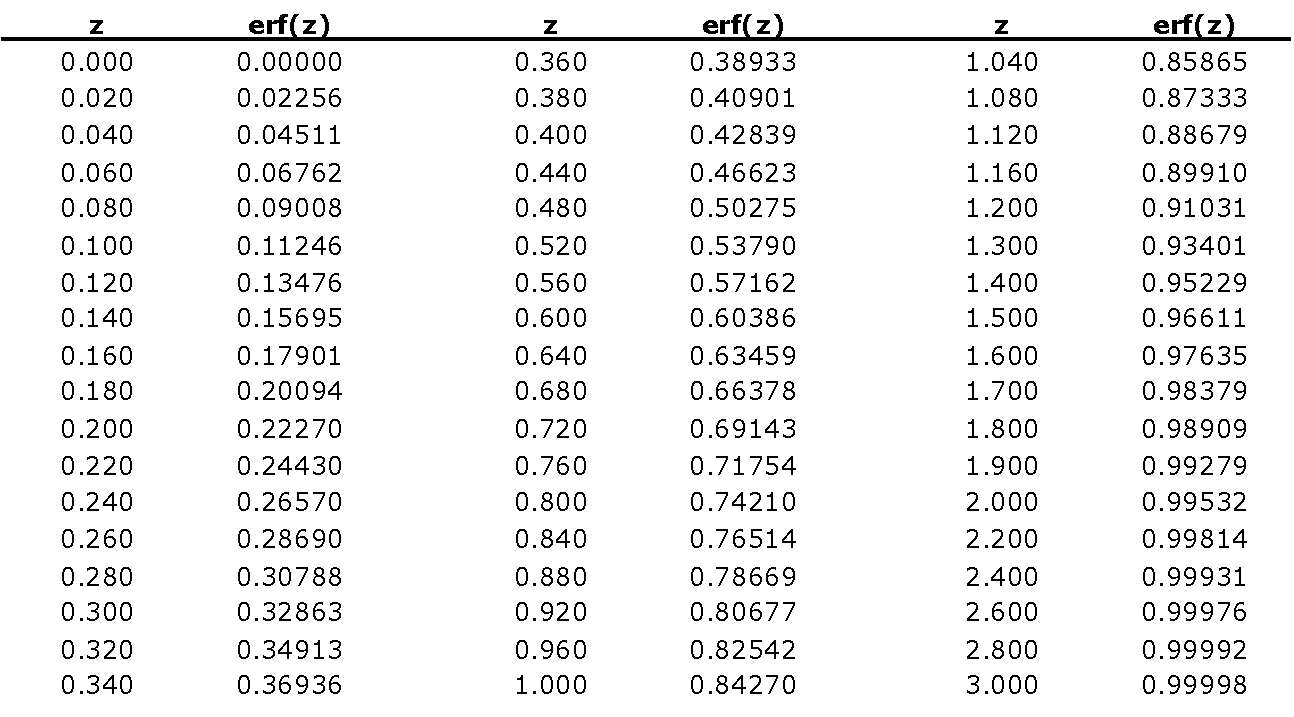
\includegraphics[width=\textwidth]{img/error_function.pdf}
    \caption{Error function look-up table}
    \label{fig:my_label}
\end{figure}


\newpage
\section{Convective Heat Transfer}
\paragraph{Convection} The energy transfer between a surface and a fluid moving over the surface.

\begin{minipage}{.4\textwidth}
    \begin{figure}[H]
    \centering
    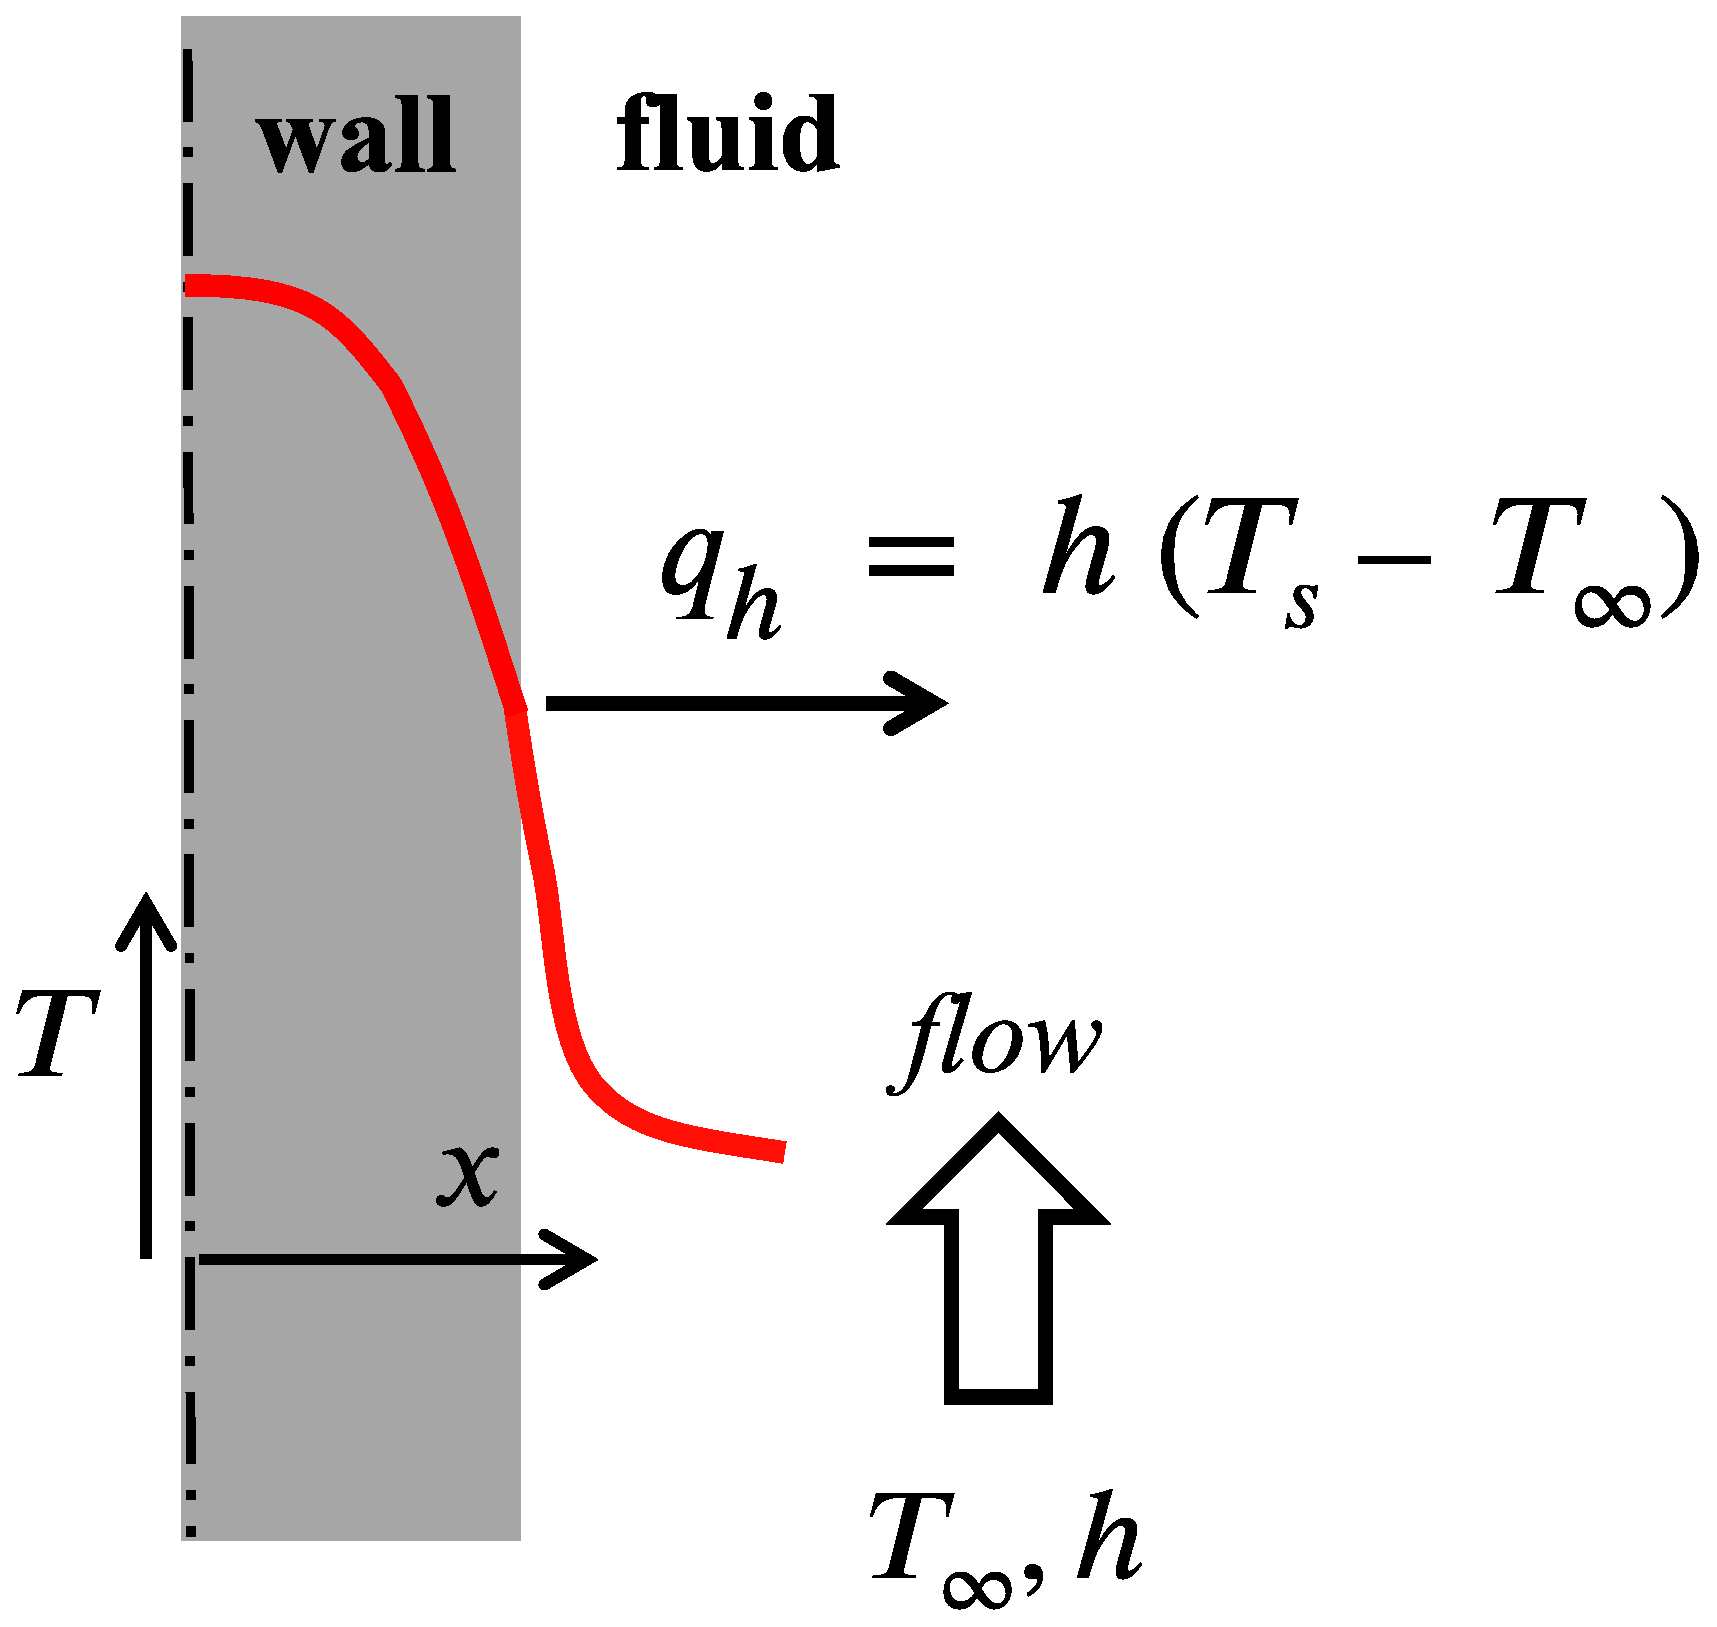
\includegraphics[width=.9\textwidth]{img/convective_heat_transfer.eps}
    \end{figure}
\end{minipage}\hfill
\begin{minipage}{.6\textwidth}
\textbf{What determines the value of the convective heat transfer coefficient, $h$?}
\begin{itemize}
    \item Fluid conductivity
    \item Fluid velocity
    \item Surface geometry
    \item Position along the surface
    \item ...
\end{itemize}
\end{minipage}
\ \\

To find the \emph{total convective heat flow, $\dot{Q}_{h}$},
\[
    \dot{Q}_{h} = \int\limits_{A_{s}} q_{h}\mathrm{d}A = (T_{s}-T_{\infty})\int\limits_{A_{s}}h\mathrm{d}A
\]
Define the \textit{average} convection coefficient, $\bar{h}$, has the following expression:
\[
    \bar{h} = \frac{1}{A_{s}}\int\limits_{A_{s}}h\mathrm{d}A_{s}
\]
Therefore,
\[
    \dot{Q}_{h} = \bar{h}A_{s}(T_{s}-T_{\infty})
\]
This expression is useful in describing convective heat transfer for a whole body.

\subsection{Boundary Layers and Heat Convective Coefficient}
Convection occurs at a surface, but how does fluid interact with the surface? This requires knowledge of boundary layers.

\subsubsection{Velocity Boundary Layer} 
Consider a uniform free-stream flow contacting a flat surface, the velocity $u$ increases from 0 at the surface (non-slip condition) to approximately $u_{\infty}$ at some distance from the surface, $\delta_{V}$.
\begin{figure}[H]
    \centering
    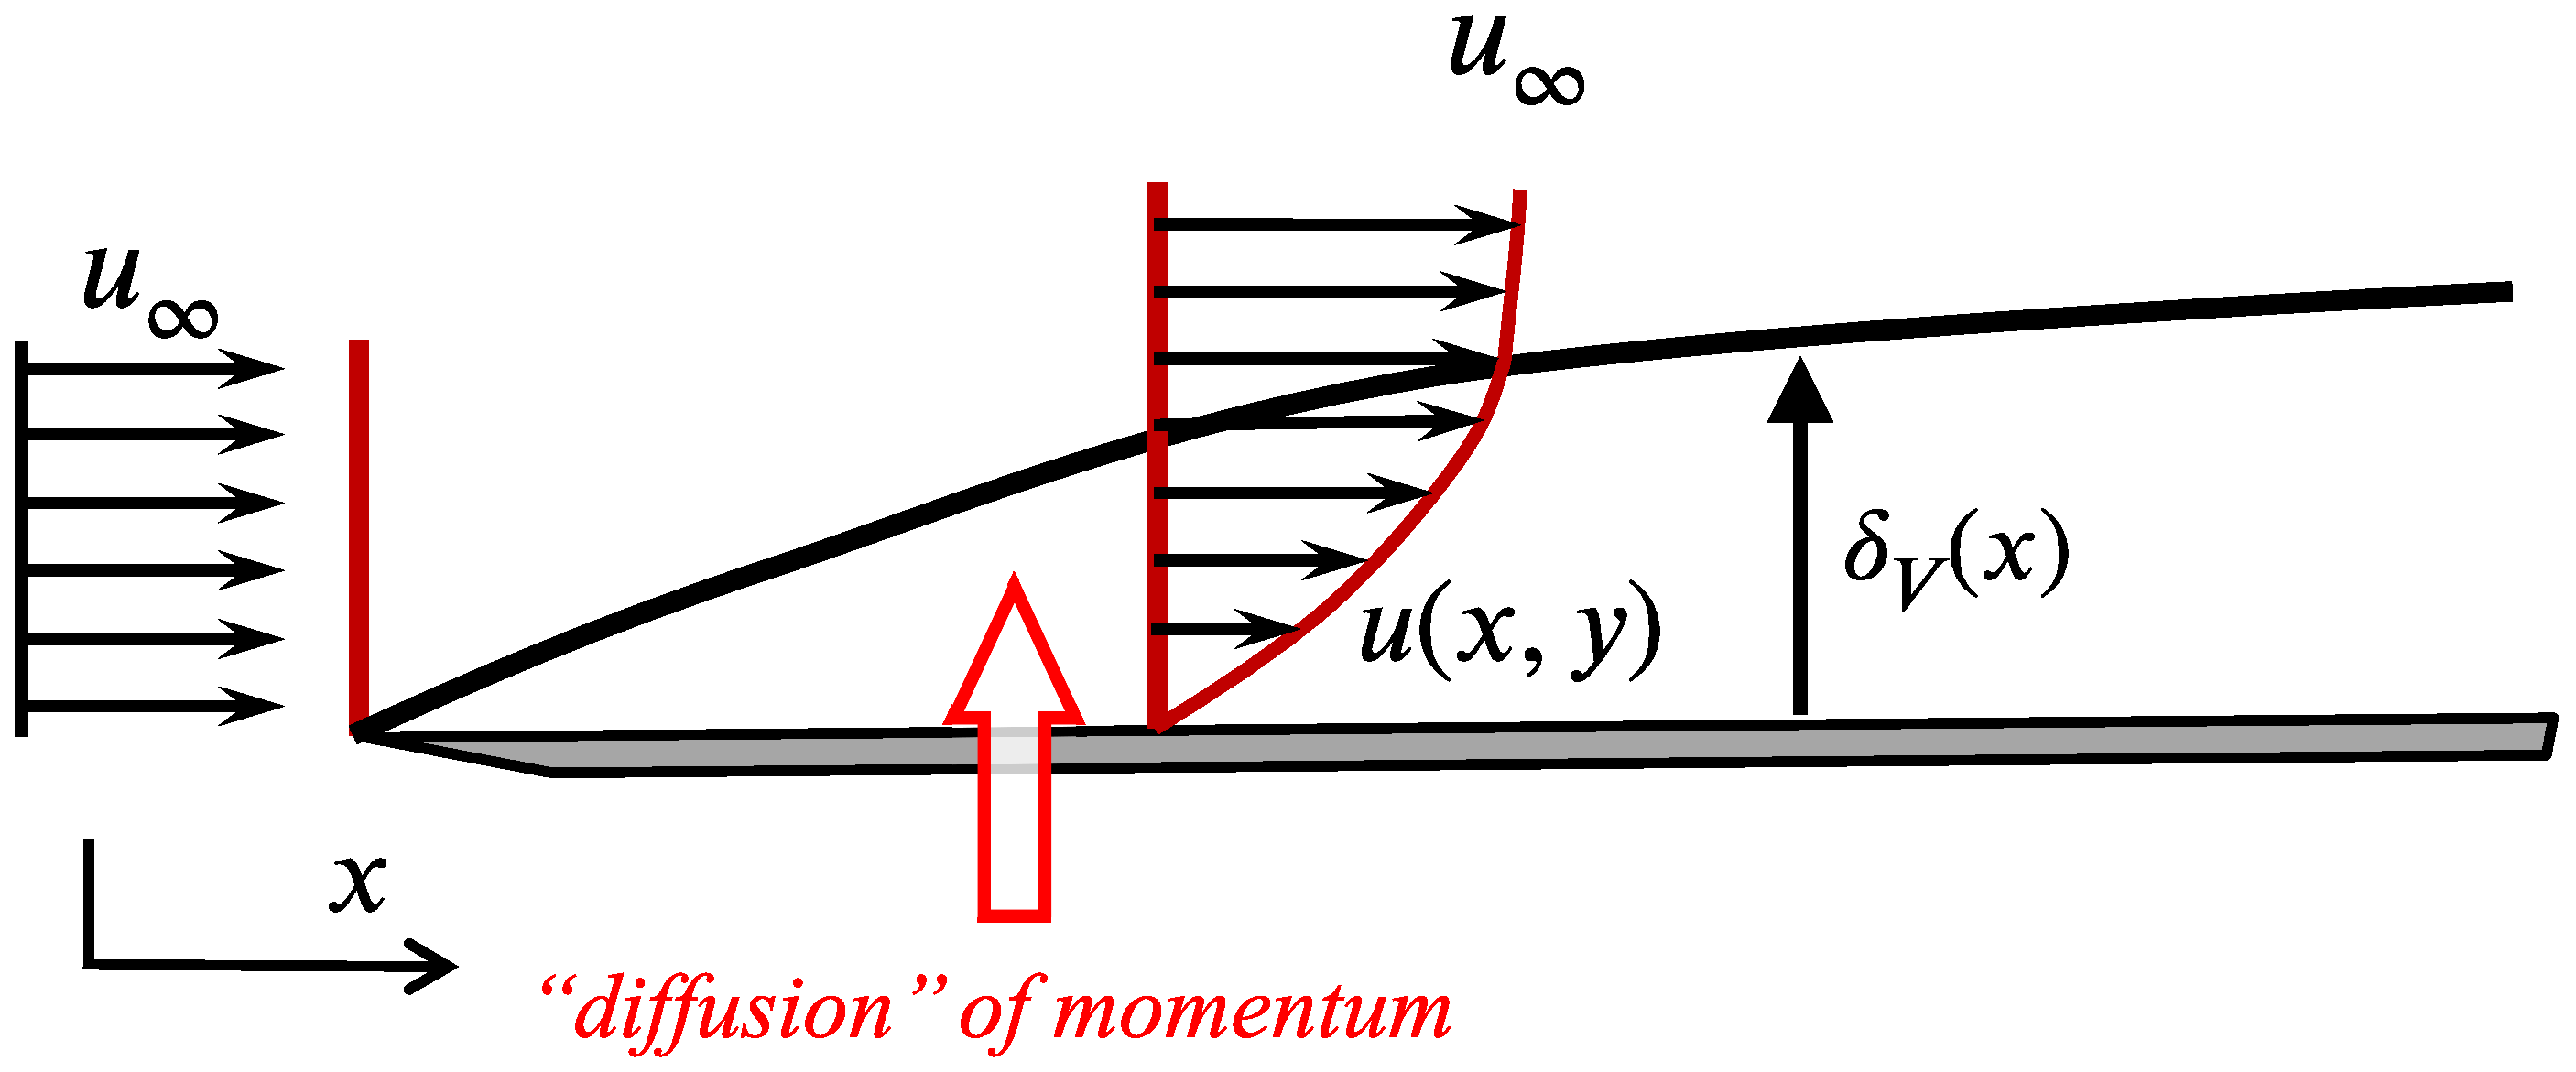
\includegraphics[width=.7\textwidth]{img/velocity_boundary_layer.eps}
    \caption{A uniform “free-stream” flow contacting a flat surface}
    \label{fig:velocity_BL}
\end{figure}
where 
\begin{itemize}
    \item[-] $u_\infty$: free stream velocity;
    \item[-] $u(x, y)$: boundary layer velocity profile;
    \item[-] $\delta_V$: velocity boundary layer thickness.
\end{itemize}

\paragraph{Velocity boundary layer thickness}  $\delta_{v} \sim \sqrt{\nu t}$, where $\nu$ is defined as \textbf{effective diffusivity} with the expression $\nu = \mu/\rho$.

\subsubsection{Thermal Boundary Layer}
Consider a uniform free-stream flow contacting an isothermal flat surface: at $y=0$, there is a thermal equilibrium between the flow and the surface; Thermal “diffusion” transfers heat through fluid. 
\begin{figure}[H]
    \centering
    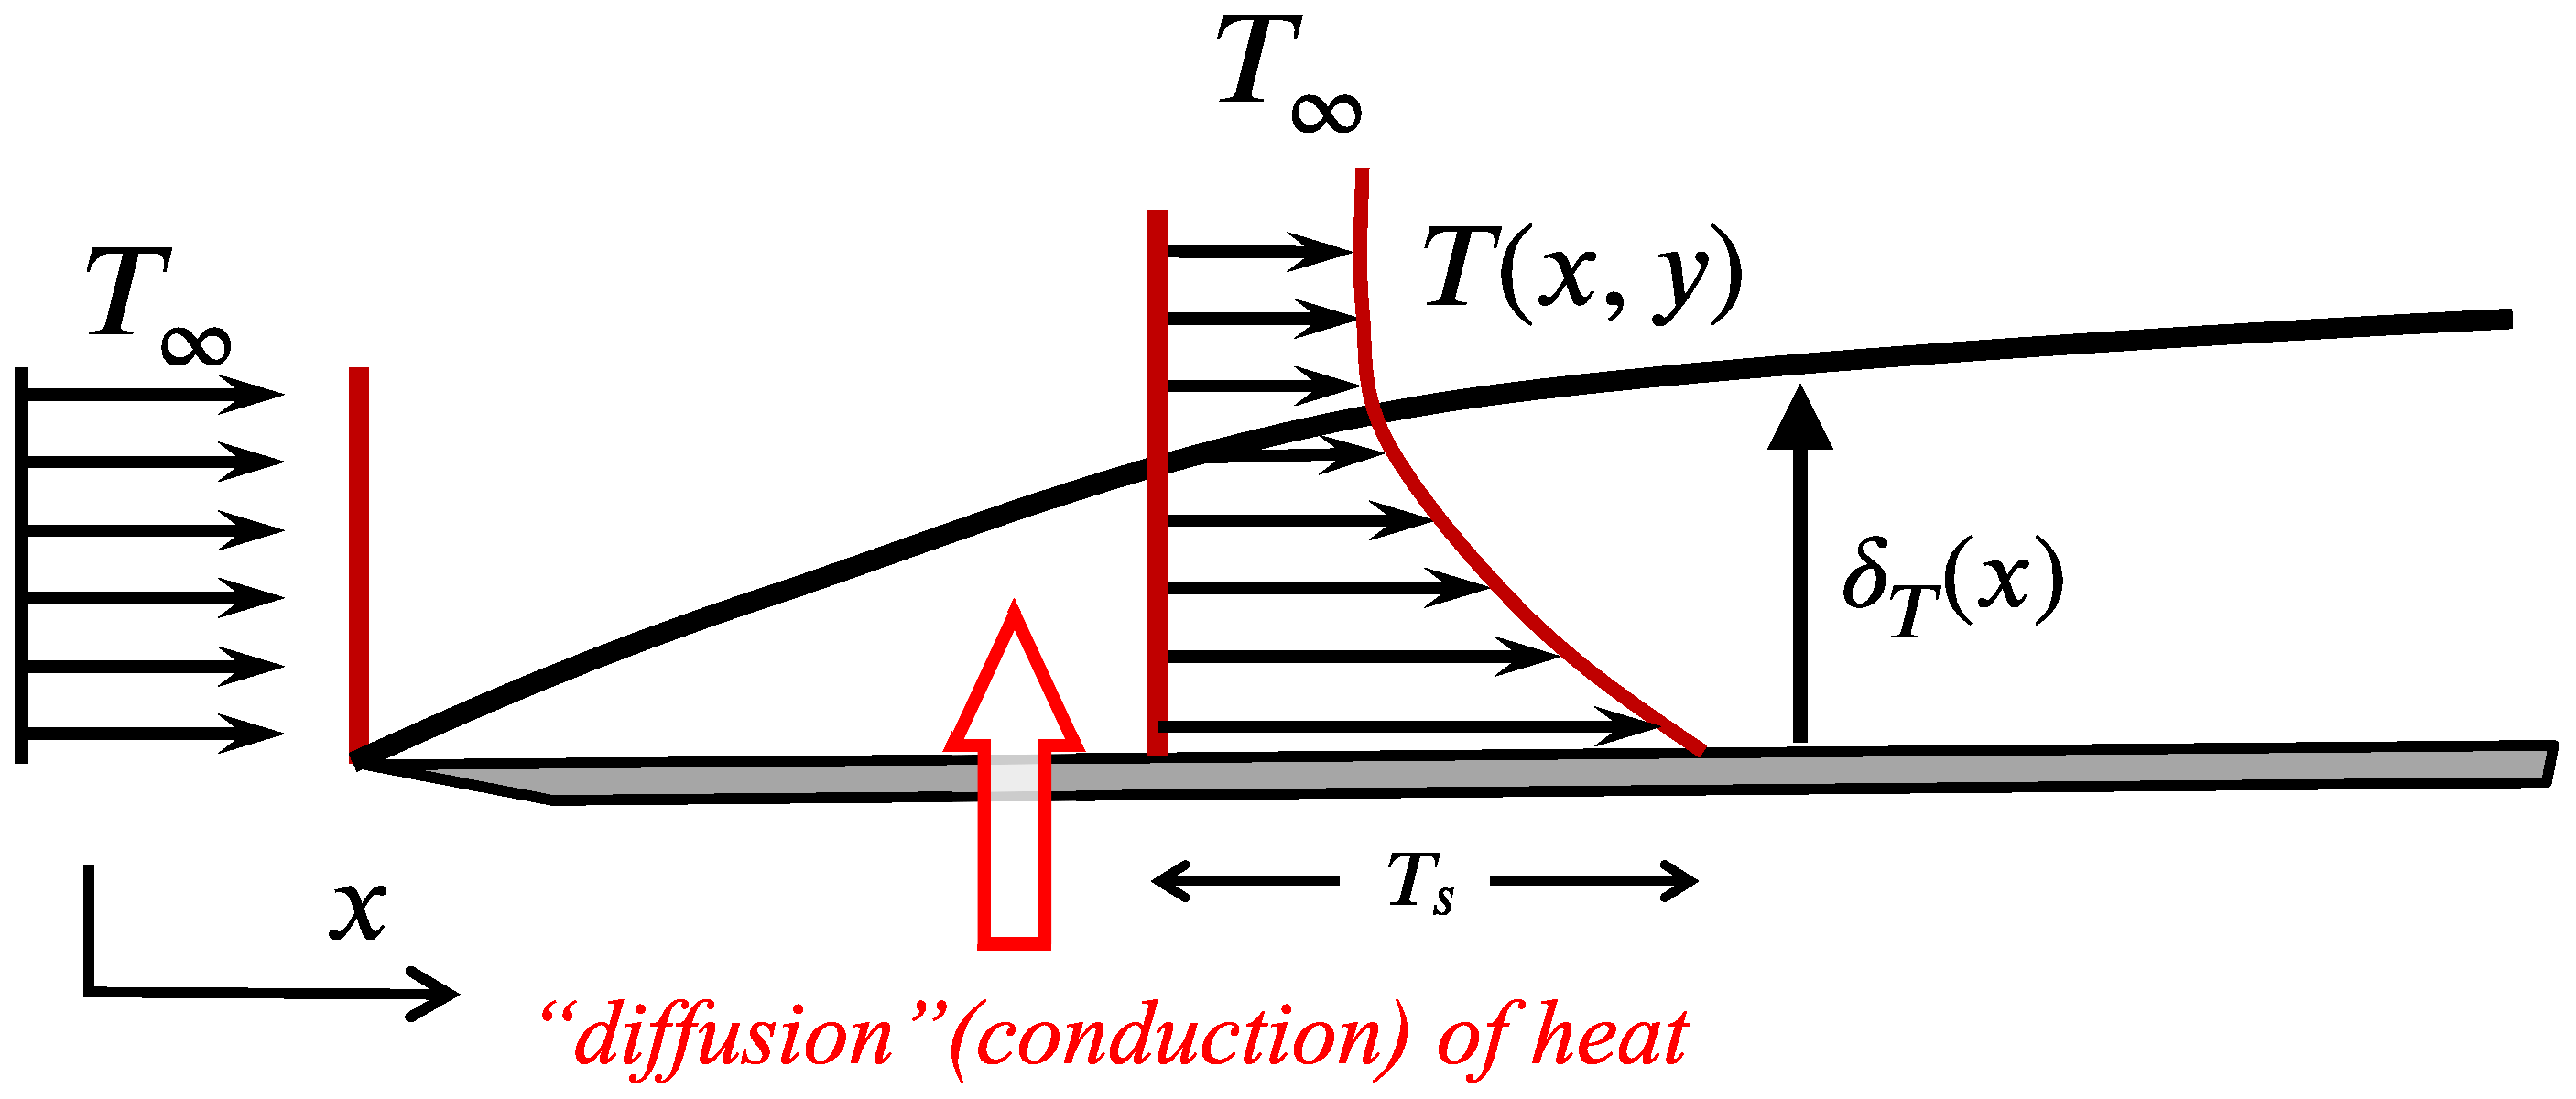
\includegraphics[width=.7\textwidth]{img/thermal_boundary_layer.eps}
    \caption{A uniform “free-stream” flow contacting a flat surface}
    \label{fig:thermal_BL}
\end{figure}
where 
\begin{itemize}
    \item[-] $T_\infty$: free stream temperature;
    \item[-] $T(x, y)$: boundary layer temperature profile;
    \item[-] $\delta_T$: temperature boundary layer thickness.
\end{itemize}

\paragraph{Thermal boundary layer thickness} $\delta_{T} \sim \sqrt{\alpha t}$, where $\alpha$ is defined as \textbf{effective diffusivity} with the expression $\alpha= k/\rho c_{p}$.\\

\textbf{Thermal and velocity boundary layers occur simultaneously!}

\subsubsection{Heat Convective Coefficient}
\paragraph{Given a thermal boundary layer, how do we calculate $h$?} At $y=0$, both convection and conduction occur, this states two fluxes must be balanced, $q_h = q_k$,
\[
    \underbrace{h(T_s-T_m)}_{q_h} = \underbrace{-k\frac{\mathrm{d}T}{\mathrm{d}y}}_{q_k} \quad \Rightarrow \quad
    h = -\frac{k}{(T_s - T_\infty)} \frac{\mathrm{d}T}{\mathrm{d}y} \bigg\lvert_{y=0} \\
\]
Define the \textit{dimensionless temperature}, $\Theta$, and the \textit{dimensionless $y$-length scale}, $y^{*}$,
\[
    \theta = \frac{T-T_\infty}{T_s-T_\infty}, \quad \quad y^{*} = \frac{y}{\delta_T}
\]
Hence,
\begin{align*}
    h 
    & = -\frac{k}{(T_s - T_\infty)} \frac{\mathrm{d}T}{\mathrm{d}y} \bigg\lvert_{y=0} \\
    & = -\frac{k}{(T_s - T_\infty)} \frac{(T_s - T_\infty)}{\delta_T} \frac{\mathrm{d}\Theta}{\mathrm{d}y^{*}} \bigg\lvert_{y=0}\\
    & = -\frac{k\sqrt{u_\infty}}{\sqrt{\alpha x}} \frac{\mathrm{d}\Theta}{\mathrm{d}y^{*}} \bigg\lvert_{y=0}\\
\end{align*}
This states
\[
    h \sim \frac{k\sqrt{u_\infty}}{\sqrt{\alpha x}} \frac{\mathrm{d}\Theta}{\mathrm{d}y^{*}}
\]
where $h$ decreases like $1/\sqrt{x}$.



\subsection{Turbulence}
\paragraph{Motivation} The first step in a convection problem is to determine whether the boundary layer is laminar or turbulent.

\paragraph{What is turbulence?}
\begin{itemize}
    \item \textbf{Laminar flow}: fluid flows in parallel layers without mixing.

    \item \textbf{Turbulent flow}: irregular, non-laminar or chaotic flow pathways with mixing.
\end{itemize}
\begin{figure}[H]
    \centering
    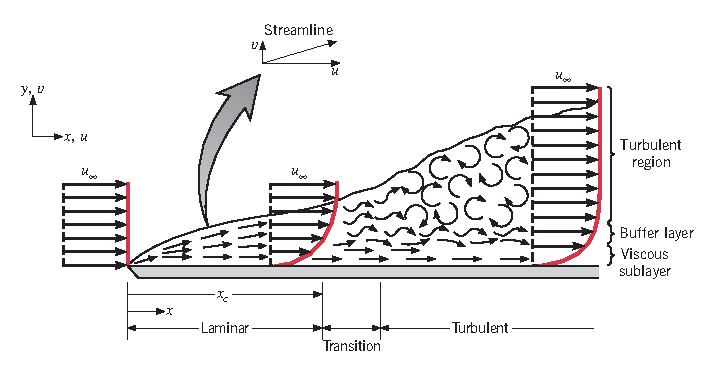
\includegraphics[width=.8\textwidth]{img/turbulence_flow_schematic.eps}
    \caption{Velocity boundary layer development on a flat plate.}
\end{figure}
\begin{figure}[H]
    \centering
    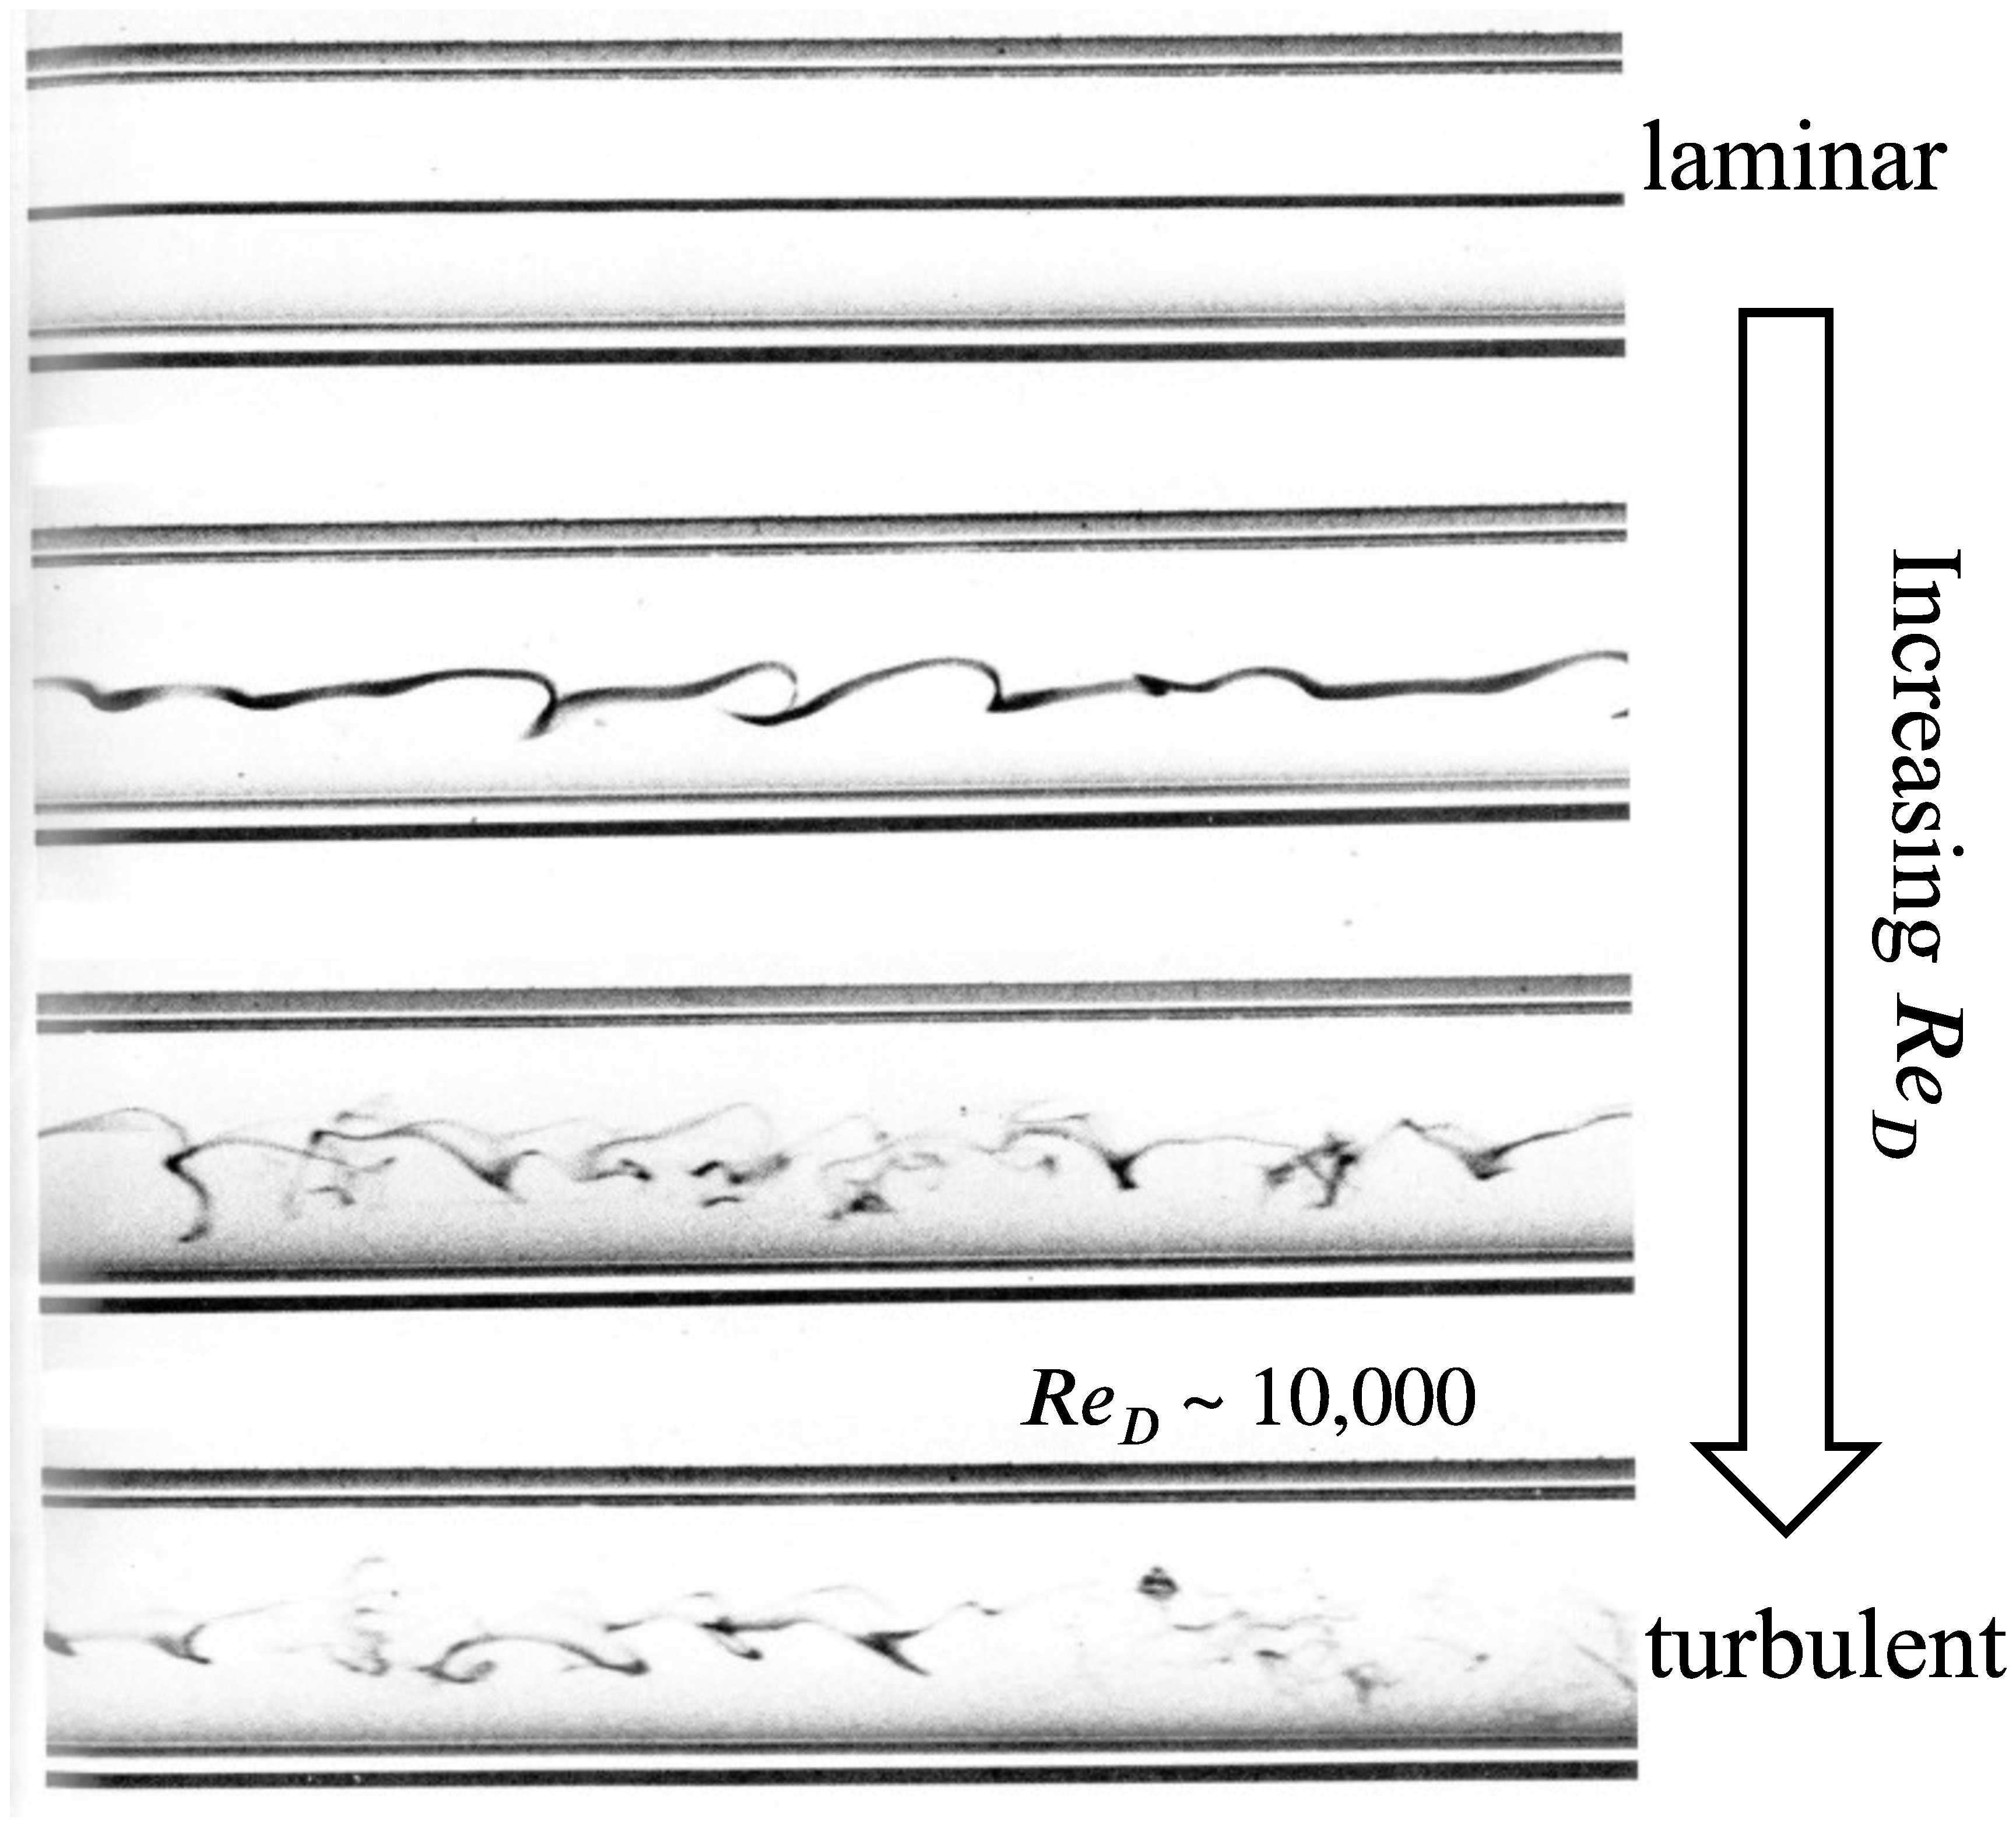
\includegraphics[width=.6\textwidth]{img/turbulence.eps}
    \caption{Turbulence in a pipe.}
\end{figure}


\begin{itemize}
    \item Boundary layer transition to turbulence after a critical length, $x_c$. \textbf{Reynolds number}, $Re$, depicts the turbulent transition:
    \[
    Re_{x} 
    = \frac{\rho u_{\infty} x}{\mu}
    = \frac{u_{\infty} x}{\nu}
\]
\end{itemize}


\subsection{Boundary Layer Thickness}
\begin{table}[H]
    \centering
    \begin{tabularx}{\textwidth}{p{.25\textwidth} p{.2\textwidth} p{.5\textwidth}}
    \toprule
        \textbf{Dimensionless Number} & \textbf{Expression} & \textbf{Description}  \\
    \midrule
        Reynolds Number & $\displaystyle Re_{x} = \frac{u_{\infty}x}{\nu}$ & ratio of internal to viscous forces \\ [1em]
        
        Prandtl Number & $\displaystyle Pr = \frac{\nu}{\alpha}$ & ratio of momentum to thermal diffusivity \\ [1em]
        
        Biot Number & $\displaystyle Bi = \frac{hL}{k}$ & ratio of conductive resistance to convective resistance (in solid) \\ [1em]
        
        Nusselt Number & $\displaystyle Nu = \frac{hL}{k}$ & dimensionless temperature gradient at surface (in fluid) \\
    \bottomrule
    \end{tabularx}
    \caption{Summary of dimensionless numbers}
    \label{tab:my_label}
\end{table}

\subsubsection{The Prandtl Number, $Pr$}
The Prandtl number, $Pr$, represents the ratio of \textit{momentum diffusivity} ($\displaystyle \nu = \frac{\mu}{\rho} \ {\color{gray}\bigg[ \frac{\mathrm{m}^2}{\mathrm{s}} \bigg]}$) to \textit{thermal diffusivity} ($\displaystyle \alpha = \frac{k}{\rho c_p} \ {\color{gray}\bigg[ \frac{\mathrm{m}^2}{\mathrm{s}}\bigg]}$). It is an intrinsic property of the fluid at a set temperature.\\

Consider external flow over a flat plate, 
\[
    \frac{\delta_V}{\delta_T} \sim \frac{\sqrt{\nu}}{\sqrt{\alpha}} = Pr^{\frac{1}{2}}
\]
thus, $Pr$ gives a physical indication of the relative thickness of the viscous boundary layer $\delta_V$ to the thermal boundary layer $\delta_T$.
\begin{figure}[H]
    \centering
    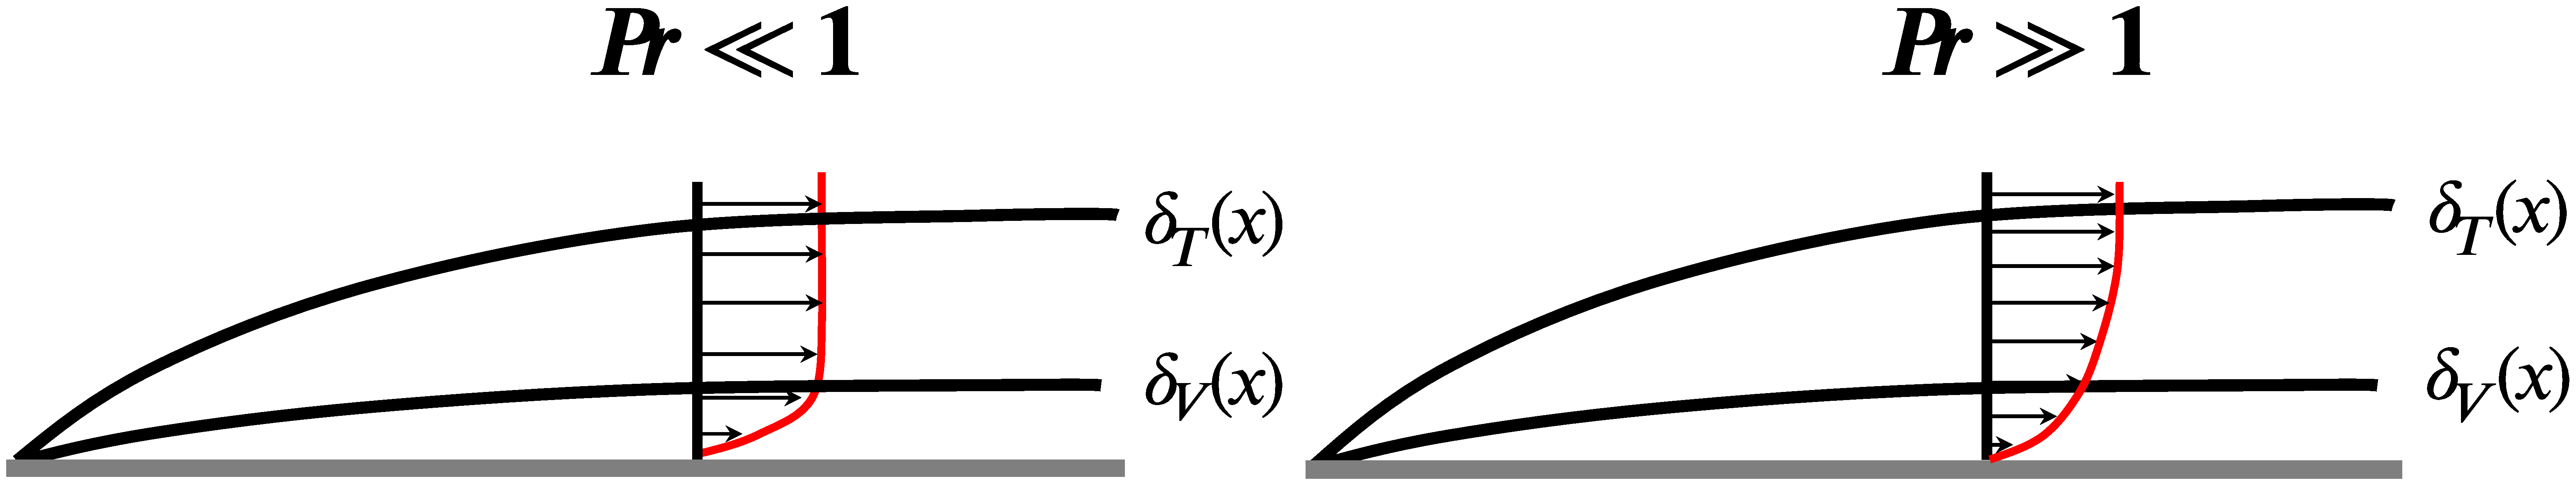
\includegraphics[width=.8\textwidth]{img/prandtl_number_boundary_layer.eps}
\end{figure}

\subsubsection{Velocity Boundary Layer Thickness, $\delta_V$}
\[
    \delta_V \sim x \ Re_{x}^{-\frac{1}{2}}
\]
\begin{tcolorbox}[breakable, title = What is the scale of $\delta_V$?]
    Neglect any thermal effects $\Rightarrow$ no change in $\nu$ and $\rho$. \\

    Momentum diffuses from a flat plate into semi-infinite fluid $\Rightarrow$ viscous penetration depth:
    \[
        \delta_V \sim \sqrt{\nu \frac{x}{u_{\infty}}}
    \]
    Re-arrange:
    \[
        \delta_V \sim \bigg( \frac{\nu \ x}{u_{\infty}} \bigg)^{\frac{1}{2}} = \underbrace{\bigg( \frac{\nu}{u_{\infty} \ x} \bigg)^{\frac{1}{2}}}_{Re^{-\frac{1}{2}}} x = \boxed{x \ Re^{-\frac{1}{2}}}
    \]
\end{tcolorbox}

\subsubsection{Thermal Boundary Layer Thickness, $\delta_T$}
\paragraph{For $Pr << 1$}
$\delta_V << \delta_T$, 
\[
    {\color{red} h \sim \frac{k}{\delta_T} \sim k \ \frac{u_{\infty}^{\frac{1}{2}}}{\alpha^{\frac{1}{2}} \ x^{\frac{1}{2}}}} \ \Rightarrow \ {\color{blue}\delta_T \sim x \bigg( \alpha \frac{x}{u_{\infty}} \bigg)^{\frac{1}{2}}}
\]
Also,
\[
    {\color{blue} \underbrace{\frac{h \ x}{k}}_{Nu_x} \sim \underbrace{\frac{u_{\infty}^{\frac{1}{2}} \ x^{\frac{1}{2}}}{\nu^{\frac{1}{2}}}}_{Re_x^{1/2}} \ \underbrace{\frac{\nu^{\frac{1}{2}}}{\alpha^{\frac{1}{2}}}}_{Pr^{1/2}}}
    \ \Rightarrow \ 
    Nu_{x} \sim Re_{x}^{\frac{1}{2}} \ Pr^{\frac{1}{2}}
\]

\paragraph{For $Pr >> 1$}
\[
    \delta_T \sim \bigg( \frac{\alpha x}{u}\bigg)^{\frac{1}{2}} \sim \bigg( \frac{\alpha \ x \ \delta_V}{u_\infty \ \delta_T}\bigg)^{\frac{1}{2}}
\]
Thus,
\[
    {\color{red}\frac{\delta_T^3}{\delta_V^3} \sim \frac{\alpha \ x}{u_\infty \ \delta_V^2} \sim \frac{\alpha \ Re_x}{u_\infty \ x} = \cancelto{1}{\frac{\nu \ Re_x}{u_\infty \ x}}\ \frac{\alpha}{\nu} \sim \frac{1}{Pr}} \ \Rightarrow \ {\color{blue}\frac{\delta_V}{\delta_T} \sim Pr^{\frac{1}{3}}}
\]
Since
\[
    \delta_V \sim x \ Re_{x}^{-\frac{1}{2}} 
\]
\[
    \delta_T \sim x \ Re^{-\frac{1}{2}} Pr^{-\frac{1}{3}}
\]

\subsection{Internal Flow}
\paragraph{Velocity entrance length} Hydrodynamic entrance length

\[
    x_{e,v} \approx 0.005 D Re_{D}
\]
\begin{figure}[H]
    \centering
    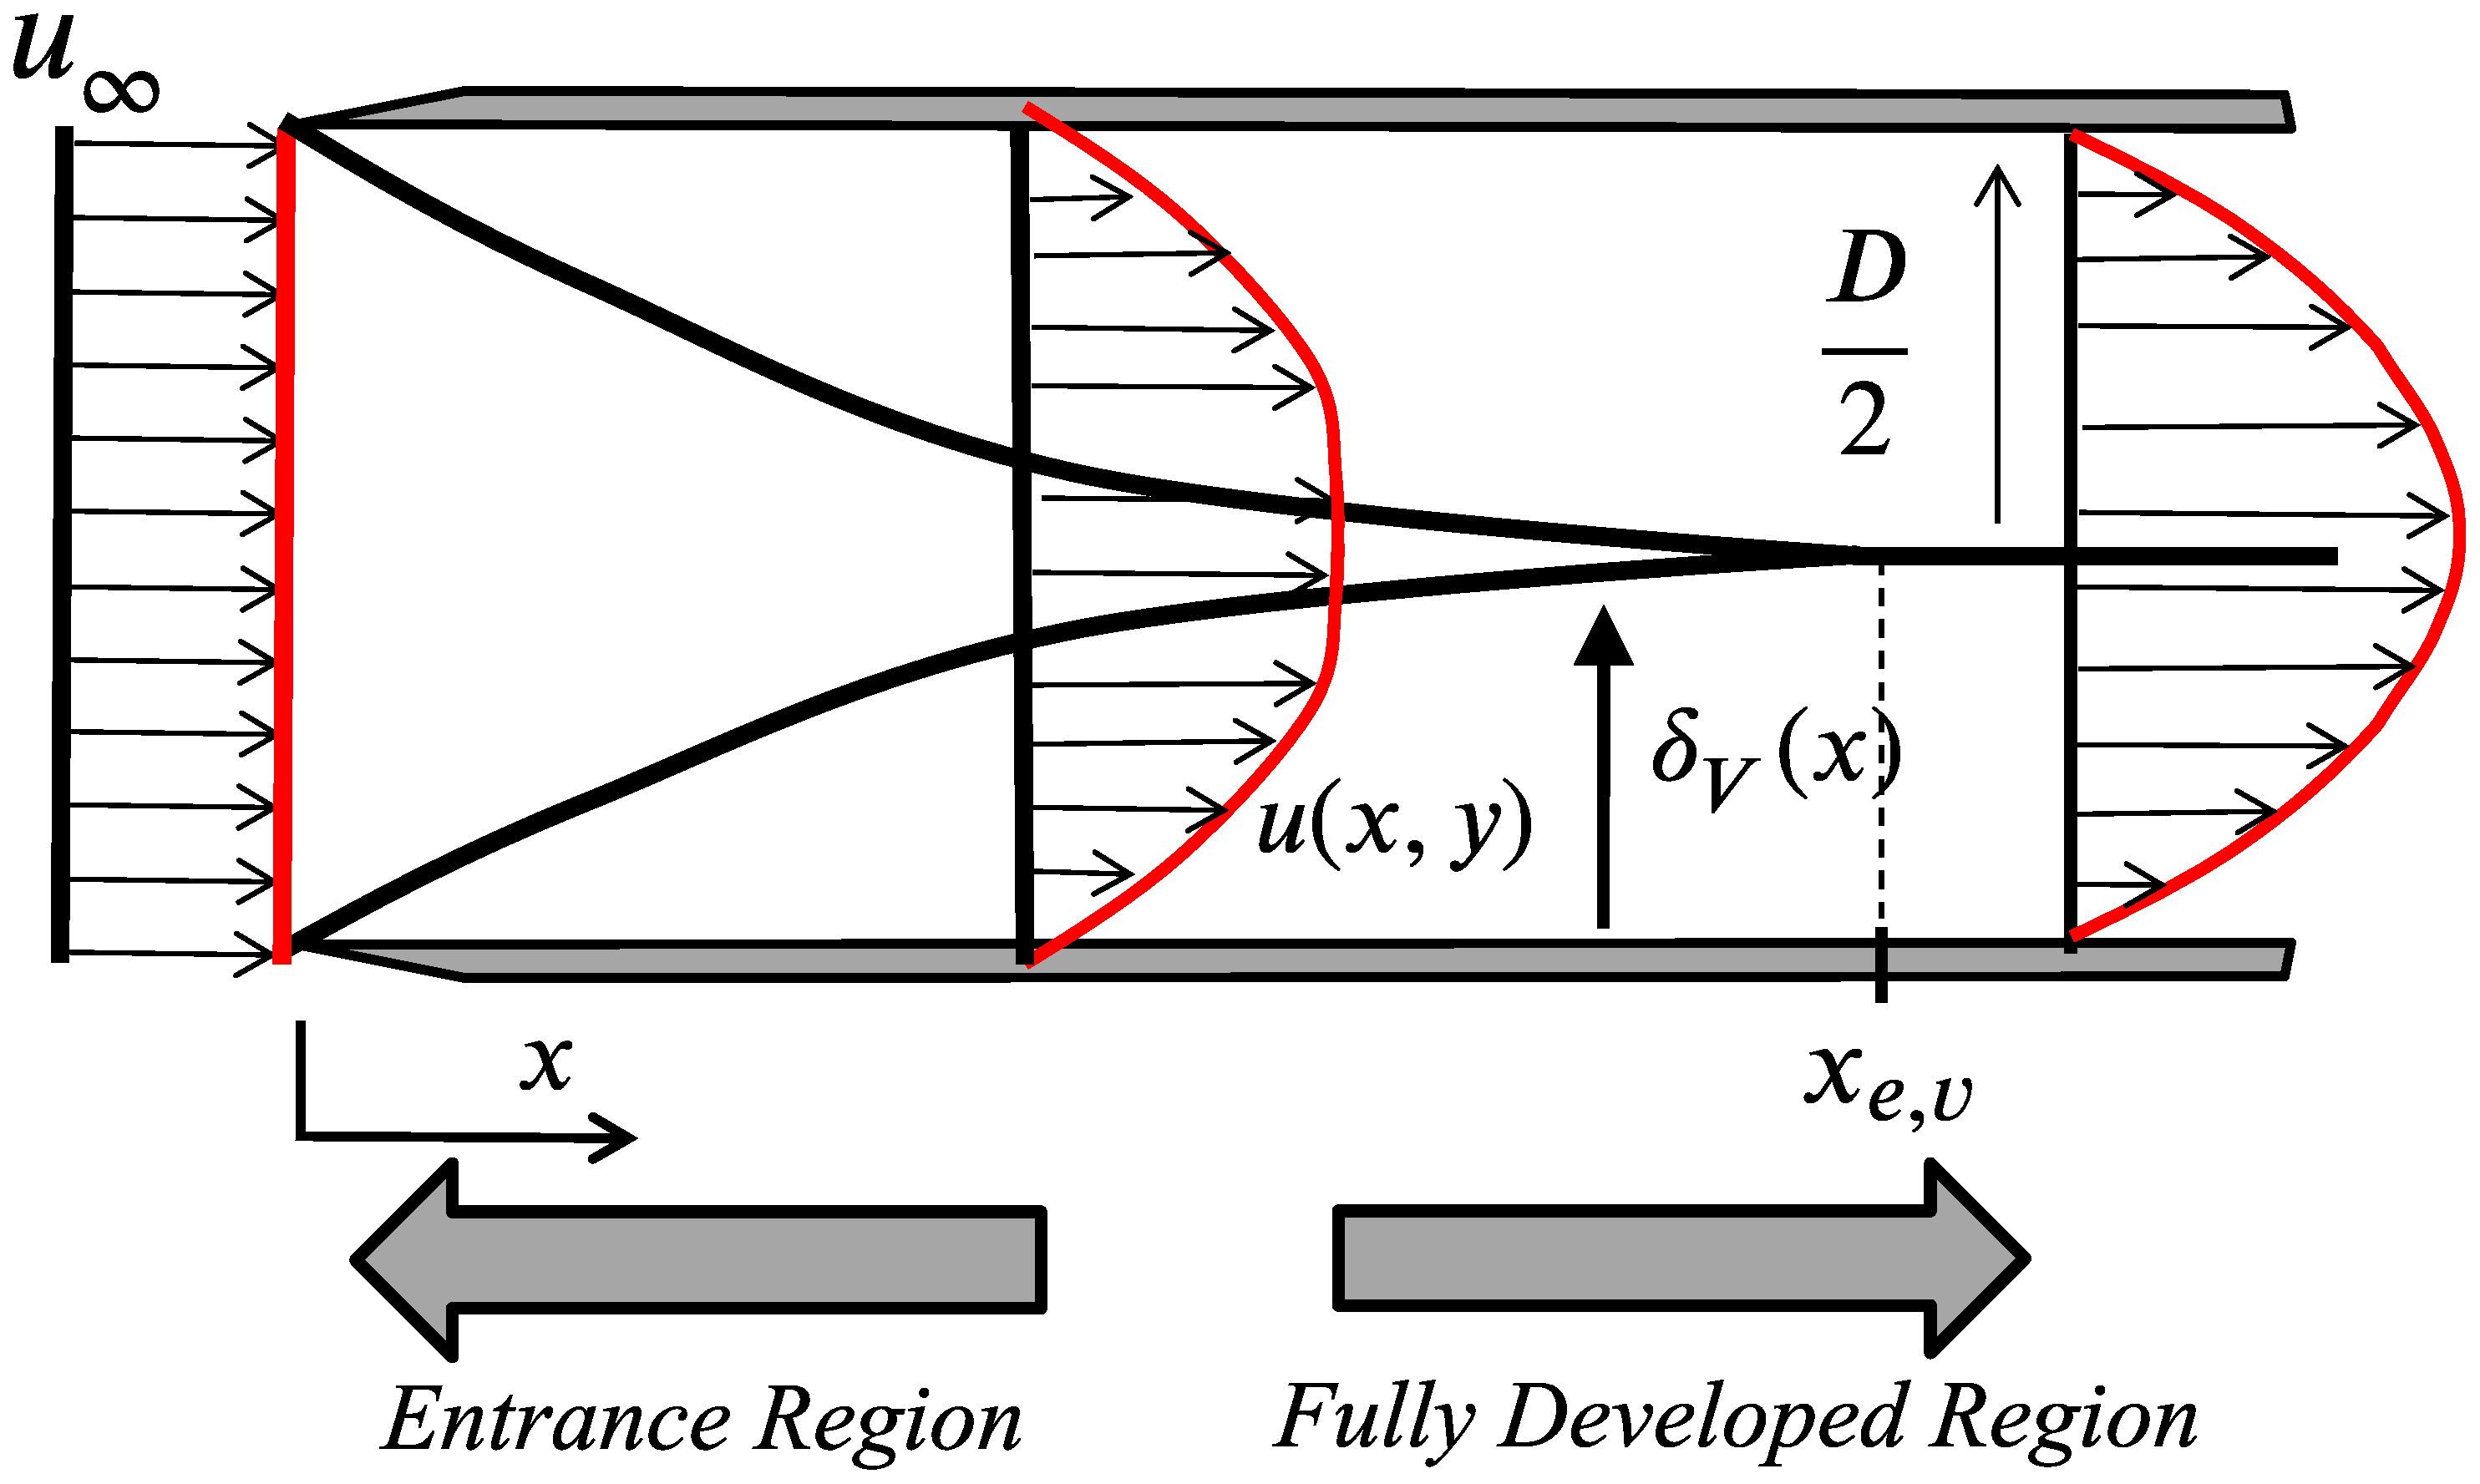
\includegraphics[width=.6\textwidth]{img/velocity_entrance_length.eps}
\end{figure}

\paragraph{Thermal entrance length}
\[
    x_{e,T} = 0.005 D Re_{D} Pr
\]
\begin{figure}[H]
    \centering
    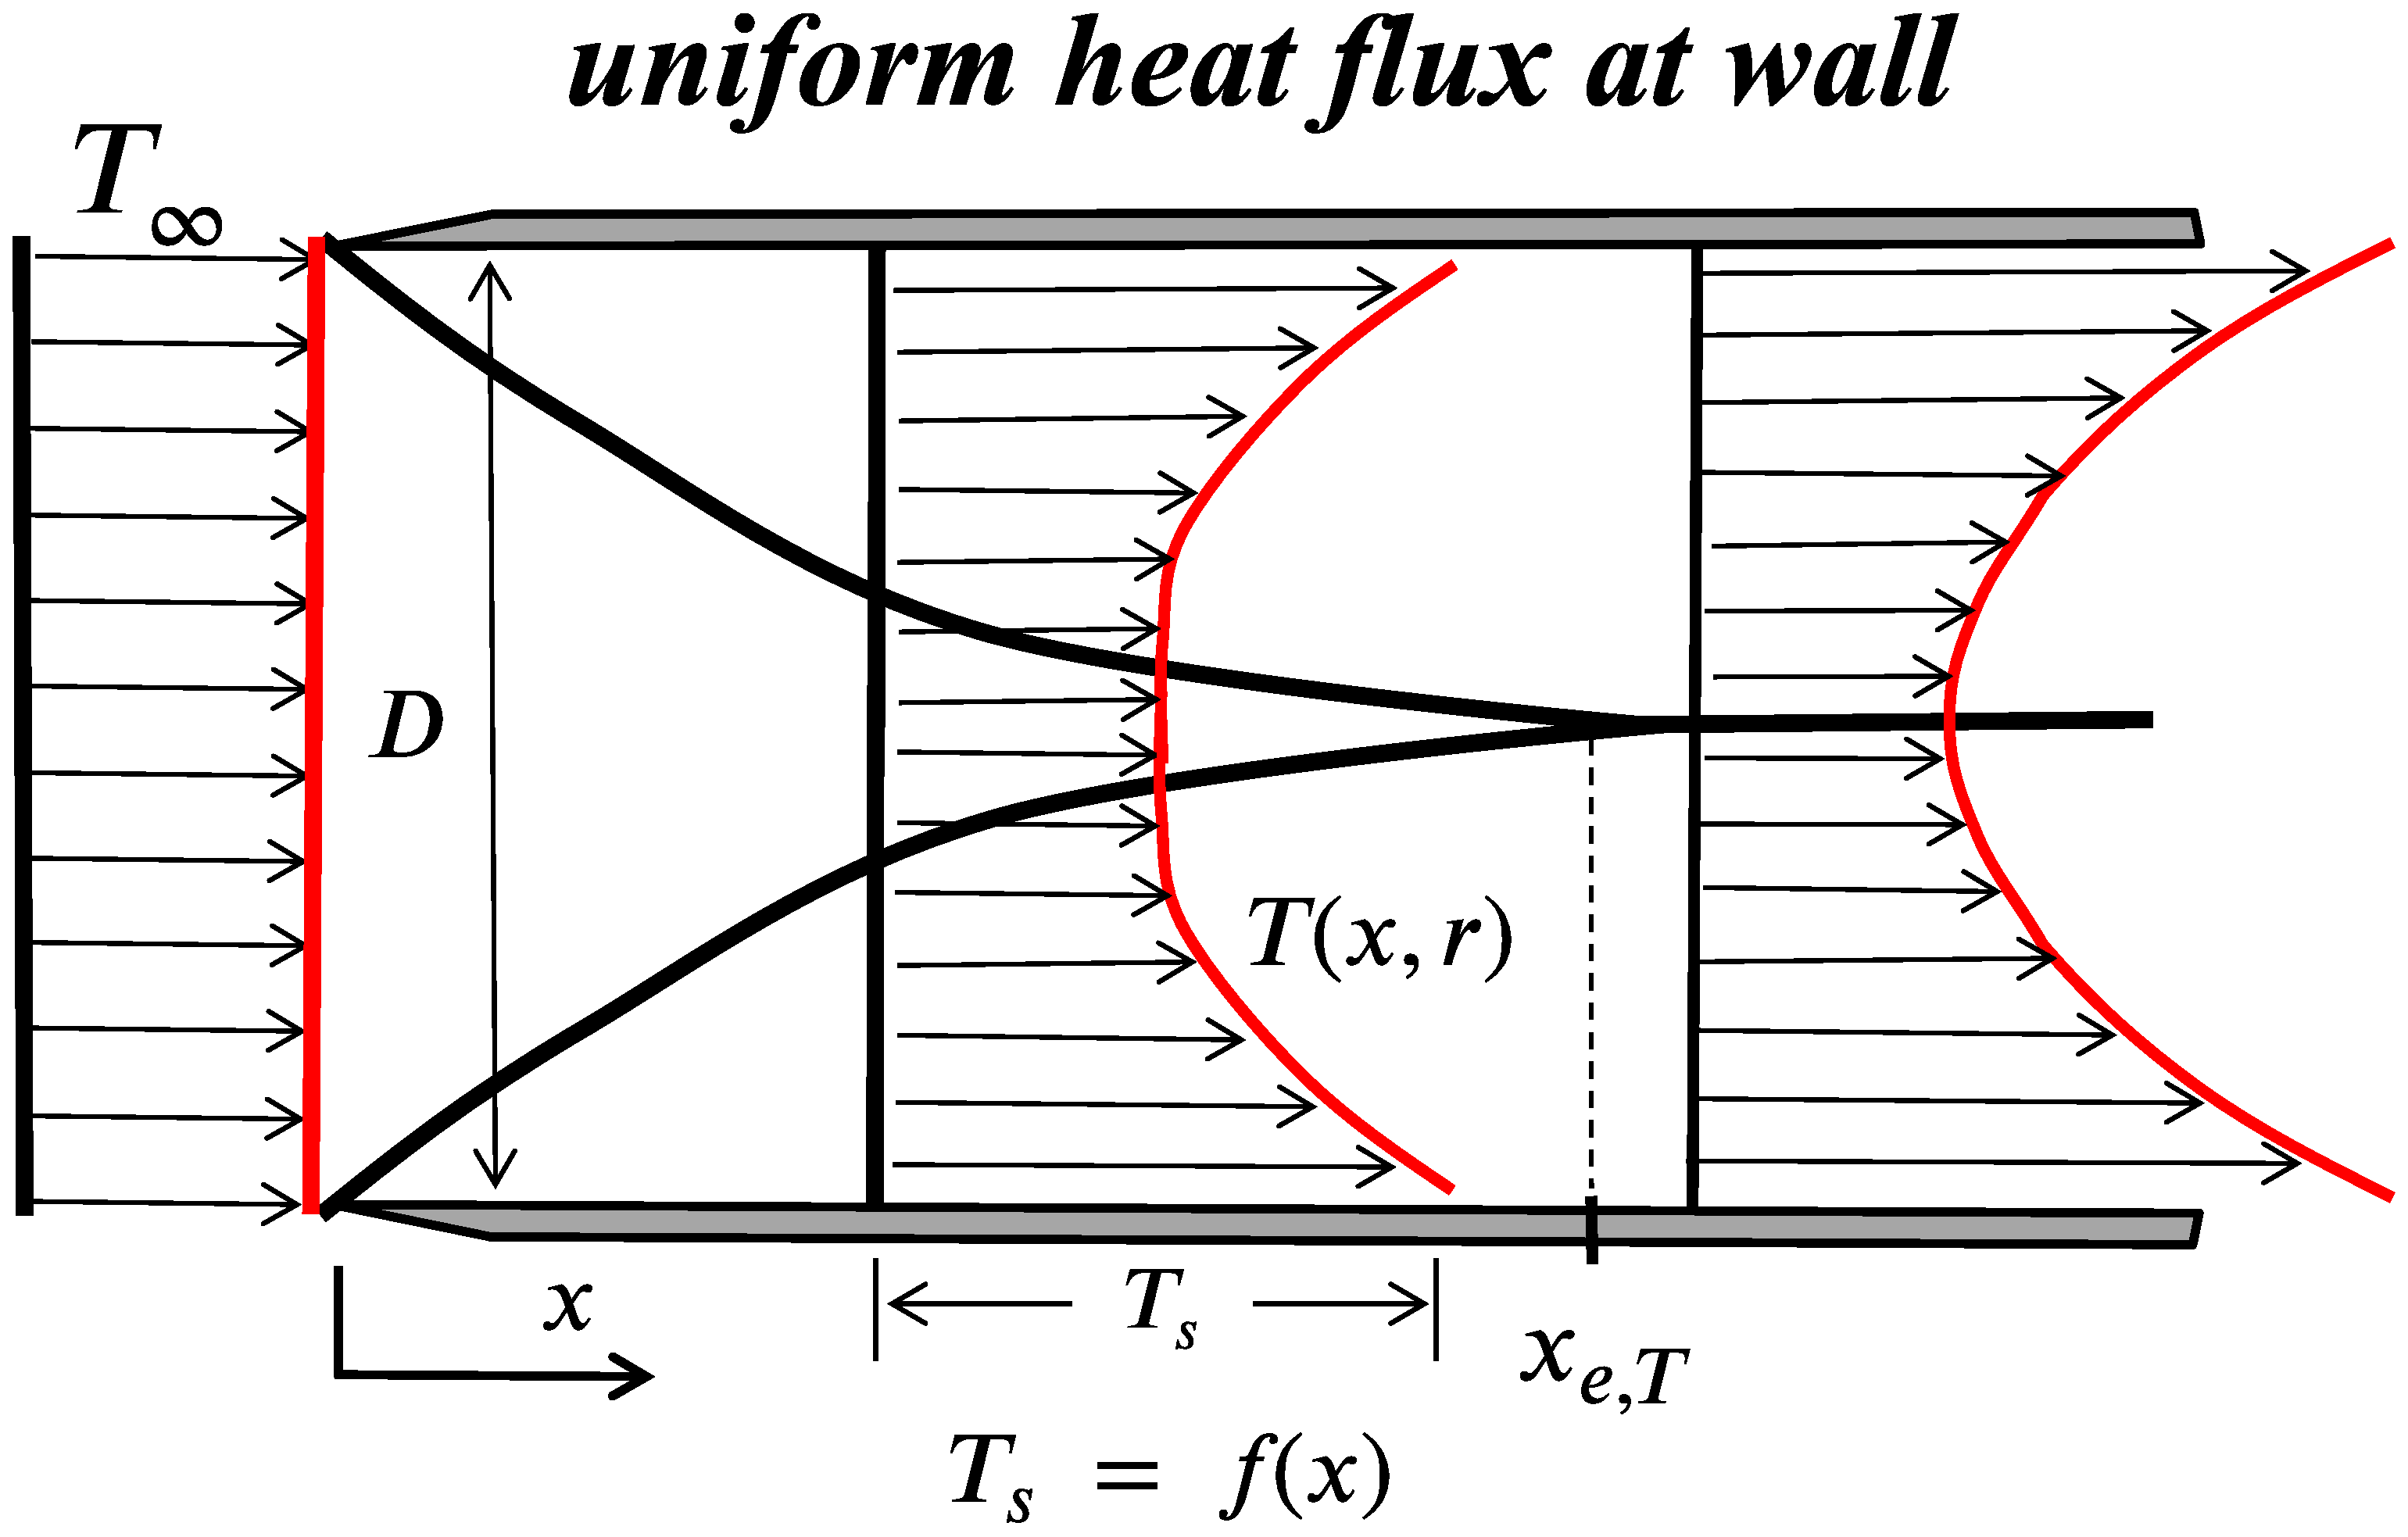
\includegraphics[width=.6\textwidth]{img/thermal_entrance_length.eps}
\end{figure}

\begin{itemize}
    \item when $x>x_{e,T}$, there is no fixed free stream temperature $T_\infty$ - a \textbf{mean} temperature, $T_m$, replaced $T_\infty$ as the reference temperature.
    \[
        T_m = \frac{2\pi}{Q} \int_{0}^{R} T u r \mathrm{d}r
    \]

    \item when the boundary layer is thermally fully developed: adding heat must increase the temperature - $T$ changed in space, not time, \textbf{general shape of the thermal profile is preserved}. \\ 
    
    Assume a constant profile,
    \begin{align*}
        \Theta' = a \bigg( 1 - \frac{r^2}{R^2} \bigg) \quad 
        & \Rightarrow \quad T = a (T_m - T_s) \bigg( 1 - \frac{r^2}{R^2} \bigg) + T_s \\
        & \Rightarrow \quad \frac{\partial T}{\partial r} = a (T_m - T_s) \bigg(- \frac{2r}{R^2} \bigg)
    \end{align*}
    
    Therefore,
    \begin{align*}
        q_r & =  h(T_m - T_s) = -k \frac{\partial T}{\partial r} \bigg\rvert_{r=R}\\
        & \Rightarrow \quad h(T_m - T_s) = \frac{2ka}{R} (T_m - T_s) \\
        & \Rightarrow \quad h = \frac{4ka}{D}
    \end{align*}
    Therefore, the Nusselt Number
    \[
        Nu_D = \frac{hD}{k} = 4a \approx 4 \quad \Rightarrow 
        \begin{cases}
            4.36, & \text{uniform surface heat flux}\\
            3.66, & \text{uniform surface temperature}
        \end{cases}
    \]
\end{itemize}


\newpage
\section{Mass Transport}
\subsection{Advection and Diffusion}

\begin{itemize}
    \item \textbf{The total flux}, $\bm{j}$, 
    \[
    \bm{j} = \bm{j}_a + \bm{j}_d
    \]
    
    \item \textbf{Advection of Solute}, $\bm{j}_a$: If the solvent undergoes bulk motion, then there will be an additional solute flux as the solute is carried along with the flow.
    \[
        \bm{j}_a = \bm{v}C
    \]
    where $C$ is the solute concentration.
    
    \item \textbf{Diffusive Flux}, $\bm{j}_d$: the diffusive flux of solute is driven by a concentration gradient.
    \[
        \bm{j}_a = -\mathcal{D}_{AB}\nabla C
    \]
        \begin{itemize}
            \item \textbf{The diffusivity}, $\mathcal{D}_{AB}$, is determined by the \textbf{Stokes-Einstein Relationship}
            \[
               \mathcal{D}_{AB} = \frac{k_{B}T}{6\pi \mu a} 
            \]
            where $k_B \approx 1.38\times 10^{-2}$ J/K is the Boltzmann's constant; and $\displaystyle a = \bigg(\frac{3M_w}{4\pi \rho N_A}\bigg)^{\frac{1}{3}}$ with $M_w$ being the molecular weight, $N_A$ is Avogadro’s number.
        \end{itemize}
\end{itemize}
\paragraph{P\`eclet number, $Pe$}
\[
    Pe = \frac{U L}{\mathcal{D}_{AB}}
\]
which states the ratio of advection to diffusion.

\subsection{The Integral and Differential Form of the Conservation of Mass}
The Integral form
\[
    \frac{\partial}{\partial t} \int\limits_{CV} C \mathrm{d}V = \int\limits_{CV} \dot{S}_v \mathrm{d}V - \oint\limits_{CS} (\bm{j}_d \cdot \hat{\bm{n}}) \mathrm{d}A - \oint\limits_{CS} C (\bm{v} \cdot \hat{\bm{n}}) \mathrm{d}A
\]
The differential form
\[
    \frac{\partial C}{\partial t} + (\bm{v} \cdot \nabla)C = \mathcal{D}\nabla^2 C + \dot{S}_{v}
\]
A special case: \textbf{Fick's Second Law} - no advection ($\bm{u}=0$) nor solute production ($\dot{S}_{v}=0$)
\[
    \frac{\partial C}{\partial t} = \mathcal{D}\nabla^2 C
\]

\end{document}